%% 
%% Copyright 2007-2025 Elsevier Ltd
%% 
%% This file is part of the 'Elsarticle Bundle'.
%% ---------------------------------------------
%% 
%% It may be distributed under the conditions of the LaTeX Project Public
%% License, either version 1.3 of this license or (at your option) any
%% later version.  The latest version of this license is in
%%    http://www.latex-project.org/lppl.txt
%% and version 1.3 or later is part of all distributions of LaTeX
%% version 1999/12/01 or later.
%% 
%% The list of all files belonging to the 'Elsarticle Bundle' is
%% given in the file `manifest.txt'.
%% 
%% Template article for Elsevier's document class `elsarticle'
%% with numbered style bibliographic references
%% SP 2008/03/01
%% $Id: elsarticle-template-num.tex 272 2025-01-09 17:36:26Z rishi $
%%
\documentclass[preprint,12pt]{elsarticle}

%% Use the option review to obtain double line spacing
%% \documentclass[authoryear,preprint,review,12pt]{elsarticle}

%% Use the options 1p,twocolumn; 3p; 3p,twocolumn; 5p; or 5p,twocolumn
%% for a journal layout:
%% \documentclass[final,1p,times]{elsarticle}
%% \documentclass[final,1p,times,twocolumn]{elsarticle}
%% \documentclass[final,3p,times]{elsarticle}
%% \documentclass[final,3p,times,twocolumn]{elsarticle}
%% \documentclass[final,5p,times]{elsarticle}
%% \documentclass[final,5p,times,twocolumn]{elsarticle}

%% For including figures, graphicx.sty has been loaded in
%% elsarticle.cls. If you prefer to use the old commands
%% please give \usepackage{epsfig}

%% The amssymb package provides various useful mathematical symbols
\usepackage{amssymb}
%% The amsmath package provides various useful equation environments.
\usepackage{amsmath}
%% The amsthm package provides extended theorem environments
%% \usepackage{amsthm}

%% The lineno packages adds line numbers. Start line numbering with
%% \begin{linenumbers}, end it with \end{linenumbers}. Or switch it on
%% for the whole article with \linenumbers.
%% \usepackage{lineno}
\usepackage{graphicx}
\usepackage{url}
\journal{Blockchain: Research and Applications}

% 1. 在导言区添加宏包
\usepackage{pdflscape}
\usepackage{pifont}

% Table 2: HCI Analysis 居中优化
\usepackage{tabularx}

% Table 3: 行业对比表最大化利用横向页面空间
\usepackage{adjustbox}

% For itemize in tables
\usepackage{enumitem}

\begin{document}

\begin{frontmatter}

%% Title, authors and addresses

\title{SuperPaymaster: A Decentralized and UX-Optimized Ethereum Gas Payment System Based on Account Abstraction}

%% use optional labels to link authors explicitly to addresses:
%% \author[label1,label2]{}
%% \affiliation[label1]{organization={},
%%             addressline={},
%%             city={},
%%             postcode={},
%%             state={},
%%             country={}}

\author[icdi]{Huifeng Jiao\corref{cor1}}
\ead{huifeng_jiao@cmu.ac.th}
\author[icdi]{Nathapon Udomlertsakul\corref{cor2}}
\ead{nathapon.u@icdi.cmu.ac.th}
\author[icdi]{Anukul Tamprasirt\corref{cor3}}
\ead{anukul@innova.or.th}
\author[aastar]{AAStar Team\corref{cor4}}
\ead{hi@aastar.io}

%% Author affiliation
\affiliation[icdi]{organization={Chiang Mai University},
                   department={International College of Digital Innovation},
                   addressline={}, 
                   city={Chiang Mai},
                   postcode={50200}, 
                   state={},
                   country={Thailand}}
\affiliation[aastar]{organization={AAStar},
                     addressline={}, 
                     city={Chiang Mai},
                     postcode={}, 
                     state={},
                     country={Thailand}}

%% Abstract
\begin{abstract}
Current blockchain gas payments impede widespread adoption due to high costs, complexity, and poor user experience (UX) rooted in Human Computer Interaction(HCI) challenges. While Account Abstraction (ERC-4337) offers potential, centralized implementations with improvements often introduce critical risks like censorship and price manipulation, undermining decentralization. This paper introduces SuperPaymaster, a novel gas payment system using ERC-4337 Paymaster and a Standardized Decentralized Service System (SDSS) to create a truly decentralized, competitive, cost-effective and user-friendly system. It directly tackles high costs, usability friction, and centralization vulnerabilities. SuperPaymaster provides an open-source framework enabling permissionless Paymaster nodes via a unified contract, fostering competition, supporting diverse ERC-20 gas tokens, and integrating with secure accounts like AirAccount via SDSS for streamlined, secure interactions. By optimizing gas payments through enhanced UX and decentralization, SuperPaymaster aims to significantly lower entry barriers, improve blockchain interaction efficiency and usability, and ultimately accelerate Web3 adoption. A Proof-of-Concept (PoC) demonstrates the system's feasibility and potential advantages.
\end{abstract}

%%Graphical abstract
%\begin{graphicalabstract}
%%\includegraphics{grabs}
%\end{graphicalabstract}

%%Research highlights
\begin{highlights}
\item We provide a comprehensive overview of existing gas payment systems on the Ethereum blockchain and analyze their inherent weaknesses.
\item We establish key guidelines and requirements for the design of a decentralized, seamless, and cost-effective gas payment system.
\item We propose a novel gas payment (sponsor) system, leveraging the Ethereum platform and an application sponsorship model to address costly and complex processes.
\item We conduct a proof of concept (PoC) to demonstrate the advantages of the proposed system over existing solutions and to outline potential future research directions.
\end{highlights}

%% Keywords
\begin{keyword}
Blockchain \sep Ethereum \sep ERC-4337 \sep Account Abstraction \sep Paymaster \sep Gas Payment \sep Transaction Fee \sep Transaction Security \sep Standardized Decentralized Service System \sep SDSS

%% PACS codes here, in the form: \PACS code \sep code

%% MSC codes here, in the form: \MSC code \sep code
%% or \MSC[2008] code \sep code (2000 is the default)

\end{keyword}

\end{frontmatter}

%% Add \usepackage{lineno} before \begin{document} and uncomment 
%% following line to enable line numbers
%% \linenumbers

%% main text
%%

%% Use \section commands to start a section
\section{Introduction}
\label{sec:introduction}

Blockchain technology, underpinning a digital asset market valued in the trillions \cite{coinmarketcap2024}, offers transformative potential for societal collaboration. However, its path to mass adoption is significantly hindered by user experience challenges, particularly surrounding the fundamental process of paying transaction fees, or "gas" on networks like Ethereum. As established by the Technology Acceptance Model (TAM)\cite{davis1989,maranguni2015} and Human-Computer Interaction (HCI)\cite{frohlich2022,shneiderman2010,norman2013,rogers2023,murray2023,preece1994,helander2014} principles, perceived ease of use is critical for adoption. Currently, interacting with blockchain often involves a cumbersome and costly gas payment process, presenting substantial barriers related to usability, efficiency, and cost\cite{ultrasoundmoney}. Users, especially newcomers, confront a steep learning curve involving numerous complex steps (often 7 steps, including exchange interactions, KYC, wallet setup, and cross-chain transfers and more), high cognitive load, and opaque procedures which are "Norman's gulf"\cite{vermeulen2013,luger2016}. These usability hurdles act as significant deterrents, preventing many from engaging with and realizing the value of decentralized applications (dApps).

\begin{figure}[htbp]
\centering
%% Use \includegraphics command to insert graphic files. Place graphics files in 
%% working directory.
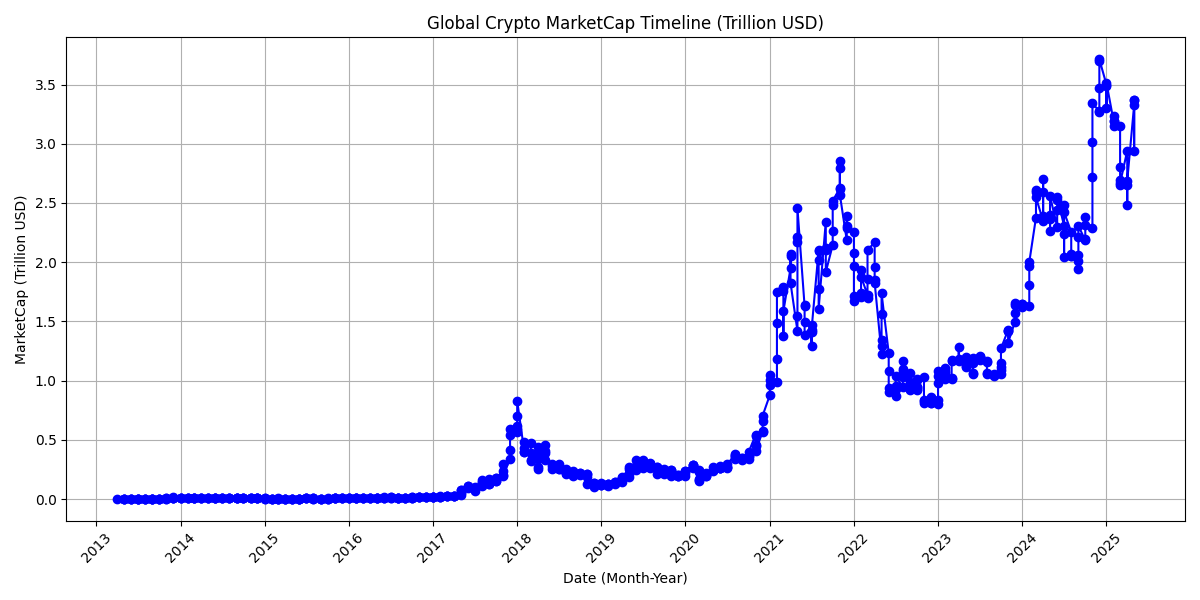
\includegraphics[width=0.8\textwidth]{crypto-market-cap-figure}
%% Use \caption command for figure caption and label.
\caption{The crypto market cap is valued in the trillions (data source: CoinMarketCap\cite{coinmarketcap2024})}
\label{fig:crypto-market-cap}
\end{figure}

The emergence of Account Abstraction (AA), particularly Ethereum's ERC-4337 standard\cite{buterin2021}, offers promising mechanisms like gas sponsorship (Paymaster) to alleviate some of these burdens. However, current implementations leveraging AA frequently introduce new centralization risks. Many rely on a limited number of centralized entities acting as Bundlers or Paymasters\cite{bundlebear2024}. This approach reintroduces vulnerabilities such as transaction censorship, potential price manipulation by dominant players, and single points of failure, directly conflicting with blockchain's core decentralization capabilities "without a trusted party"\cite{zarrin2021,nakamoto2008}. Furthermore, practical limitations persist in these centralized solutions, including restricted support for diverse ERC-20 tokens as gas payment, lack of truly permissionless service operation, and complex integration efforts for dApp developers, leaving a critical gap for a genuinely decentralized alternative.

In this paper, we introduce SuperPaymaster, a gas payment system based on ERC-4337 Account Abstraction and a novel Standardized Decentralized Service System (SDSS) architecture. SuperPaymaster is designed to foster a truly decentralized, competitive, and user-friendly system for managing transaction fees. It directly addresses the limitations of previous approaches by enabling an open-source framework where anyone can permissionlessly operate Paymaster nodes. These nodes register via SDSS (using ENS for discovery) and compete to offer gas sponsorship, facilitating lower costs and accepting a wide variety of community-issued or standard ERC-20 tokens. Integration with user-centric wallets like AirAccount further enhances usability and security, aiming for a seamless payment experience. By decentralizing the paymaster layer and prioritizing user experience through intuitive design principles that leverage familiar user paradigms, SuperPaymaster seeks to significantly lower entry barriers, improve interaction efficiency, and accelerate the broader adoption of Web3 technologies. We create a team in two years ago and delivery a Proof-of-Concept (PoC) to test the system's feasibility.

\section{Analysis of Current Gas Payment Systems and Associated Challenges}
\label{sec:analysis}

This section delves into the foundational aspects of gas payment mechanisms within EVM-compatible blockchains, outlines the typical user workflow, and critically examines the multifaceted challenges and vulnerabilities inherent in current systems, including usability barriers and the specific risks associated with centralized solutions.

\subsection{The Gas Payment Mechanism}
\label{subsec:gas-mechanism}

\subsubsection{Necessity of Gas Payment}

The requirement for users to pay 'gas' for transactions is fundamental to the operation and security of public, permissionless blockchains like Ethereum. Due to the Turing-completeness of the Ethereum Virtual Machine (EVM)\cite{wood2014}, which allows for arbitrary computation, a mechanism is needed to prevent infinite loops and denial-of-service (DoS) attacks that could exhaust network resources\cite{wood2014}. Gas acts as a computational metering unit, assigning a cost to each operational step executed by the EVM. By requiring payment for computation, the gas mechanism ensures the sustainable use of shared public resources, prevents network abuse, and incentivizes validators (miners/stakers) to process transactions and secure the network\cite{buterin2013}.

\subsubsection{Current Gas Payment Workflow}

Executing a transaction on current blockchain systems typically involves a complex, multi-step workflow for the user, even before the core on-chain interaction occurs. A user often needs to: (1) Create an account on a centralized exchange (CEX); (2) Complete Know Your Customer (KYC) verification; (3) Purchase the blockchain's native token (e.g., ETH for Ethereum) using fiat currency; (4) Set up a self-custodial wallet (e.g., MetaMask); (5) Transfer the native token from the CEX to their wallet, incurring withdrawal fees; (6) Potentially perform cross-chain swaps or bridging if operating on a different network or requiring specific tokens, adding further complexity and cost; (7) Finally, initiate the desired transaction (e.g., interacting with a dApp or wallet), requiring careful setting of gas parameters (gas limit, gas price/priority fee) and signing with their private key. This intricate process serves as a significant initial barrier, particularly for non-technical users. As we draw below, there will be over 7 steps in real world comparing with SuperPaymaster with 4 steps(s1,s2 is one time setup, s3 submit transaction, s4 view transaction result).

\begin{figure}[htbp]
\centering
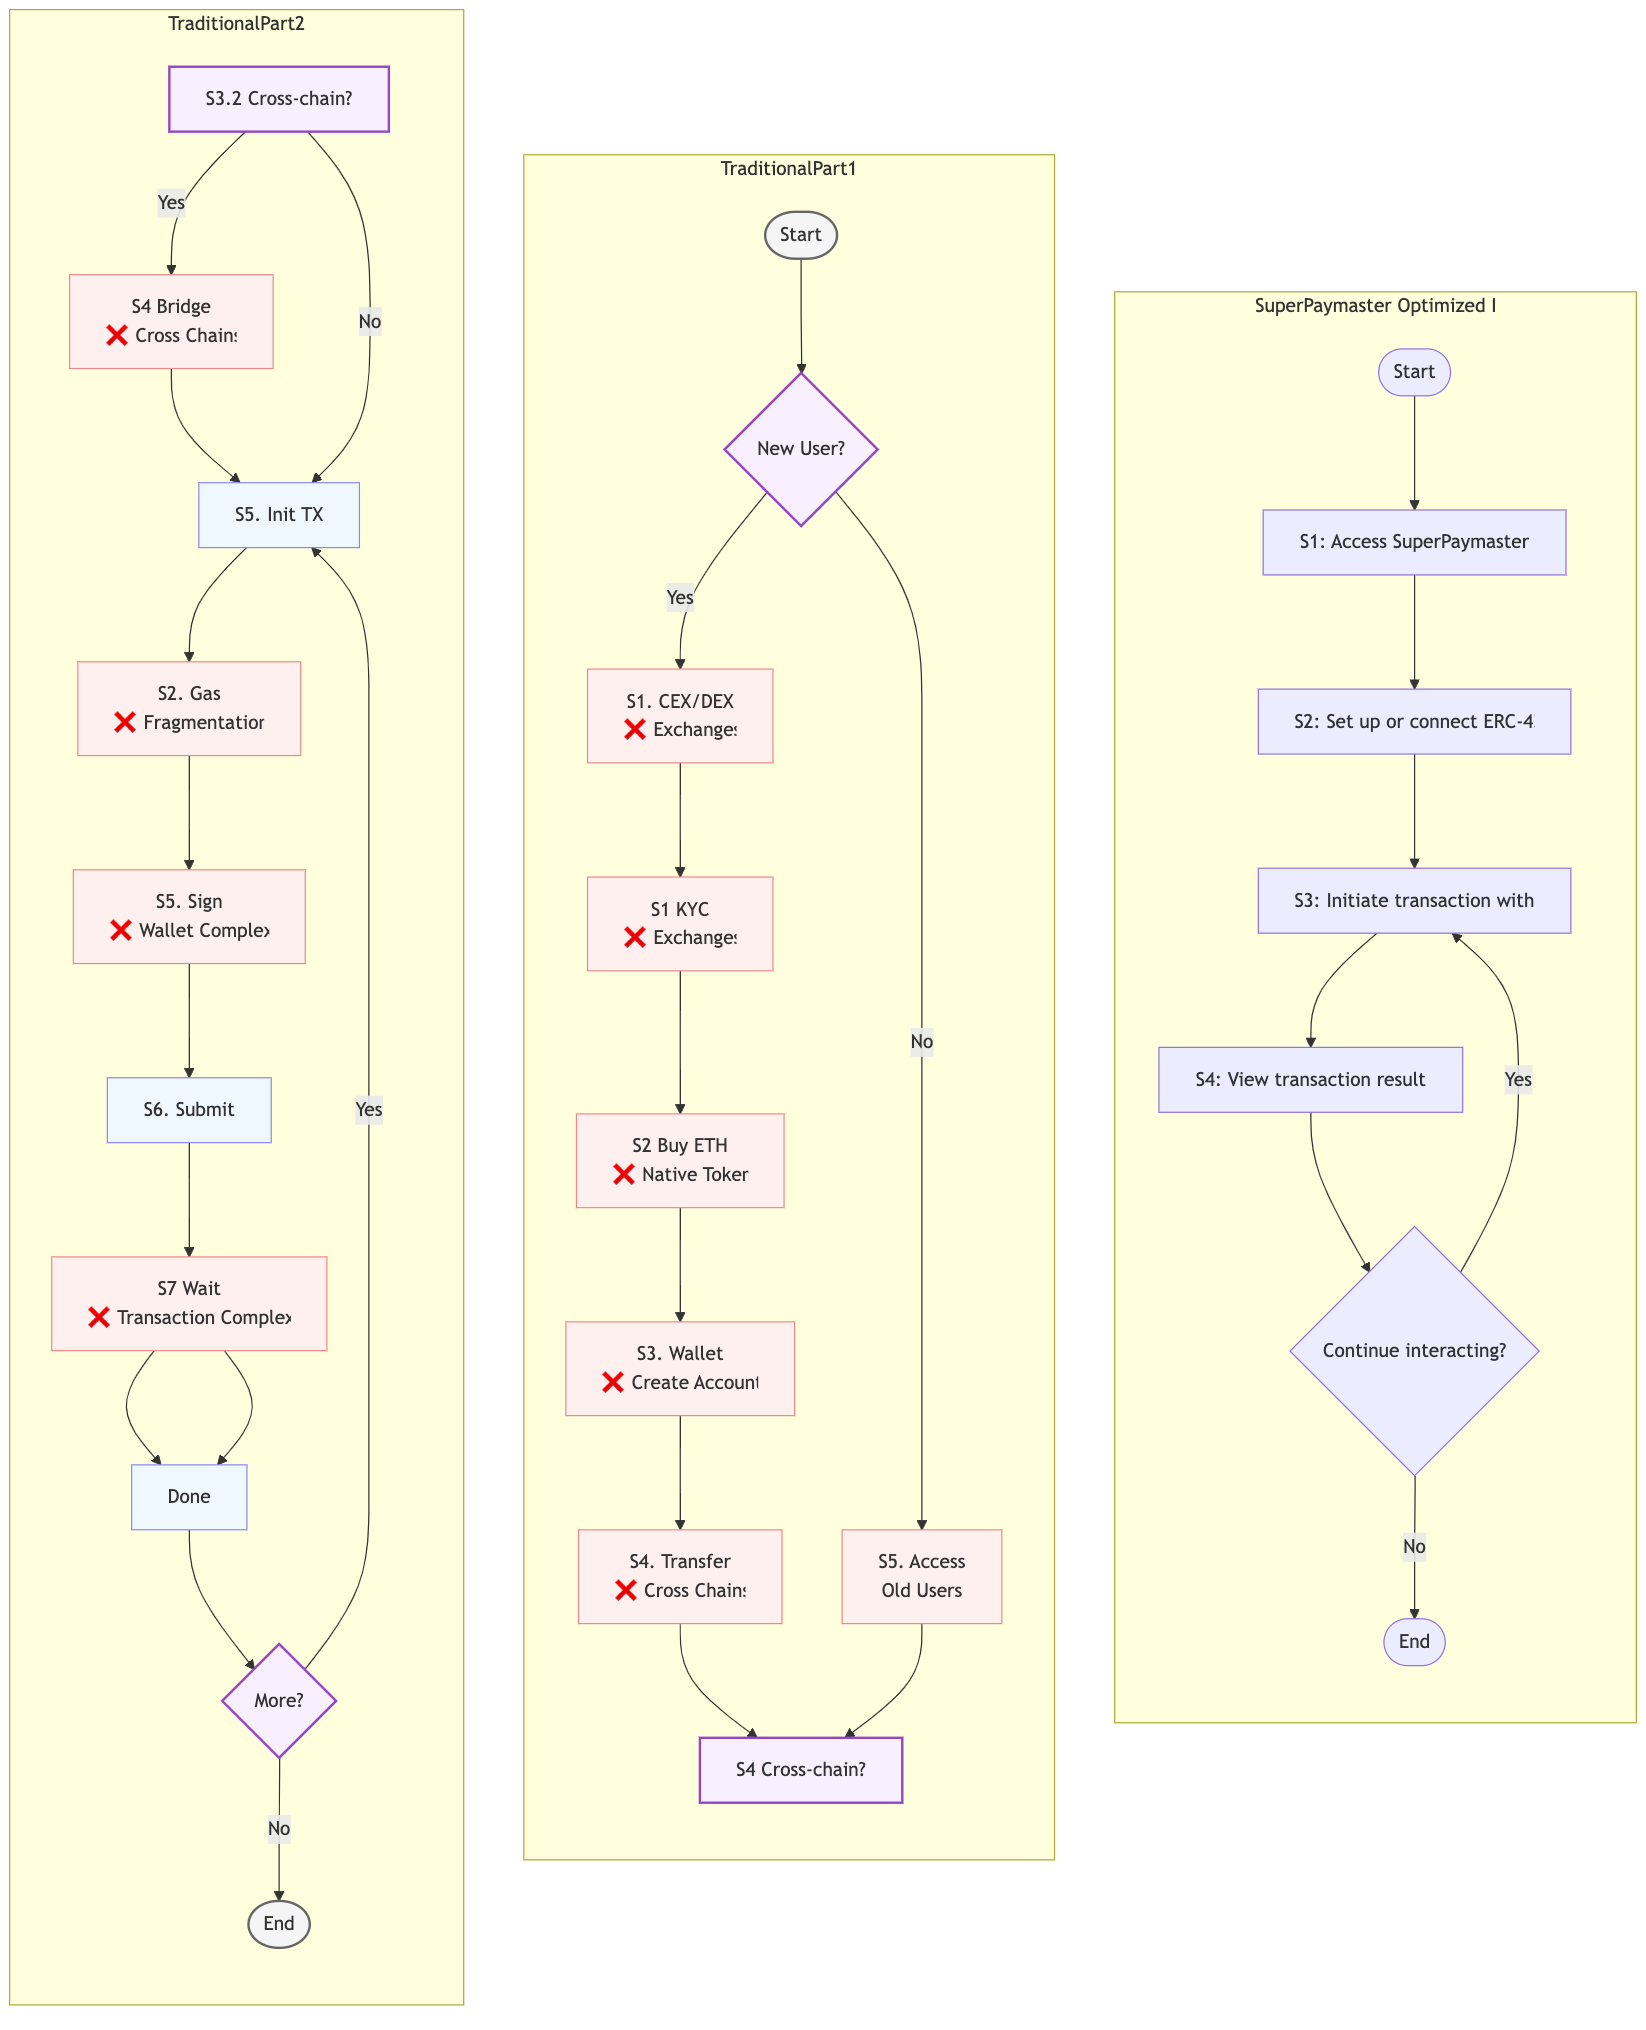
\includegraphics[width=0.8\textwidth]{paymaster-flow-comparison-figure}
\caption{Paymaster and SuperPaymaster System Flow Overview}
\label{fig:paymaster-flow-comparison}
\end{figure}

\subsection{Challenges and Vulnerabilities in Current Systems}
\label{subsec:challenges}

Existing gas payment systems suffer from a confluence of issues that impede usability, efficiency, and security. Despite promising developments like ERC-4337, current solutions for gas payments offer only partial relief, still burdening users with the need to hold native tokens and manage underlying complexities.

\begin{figure}[htbp]
\centering
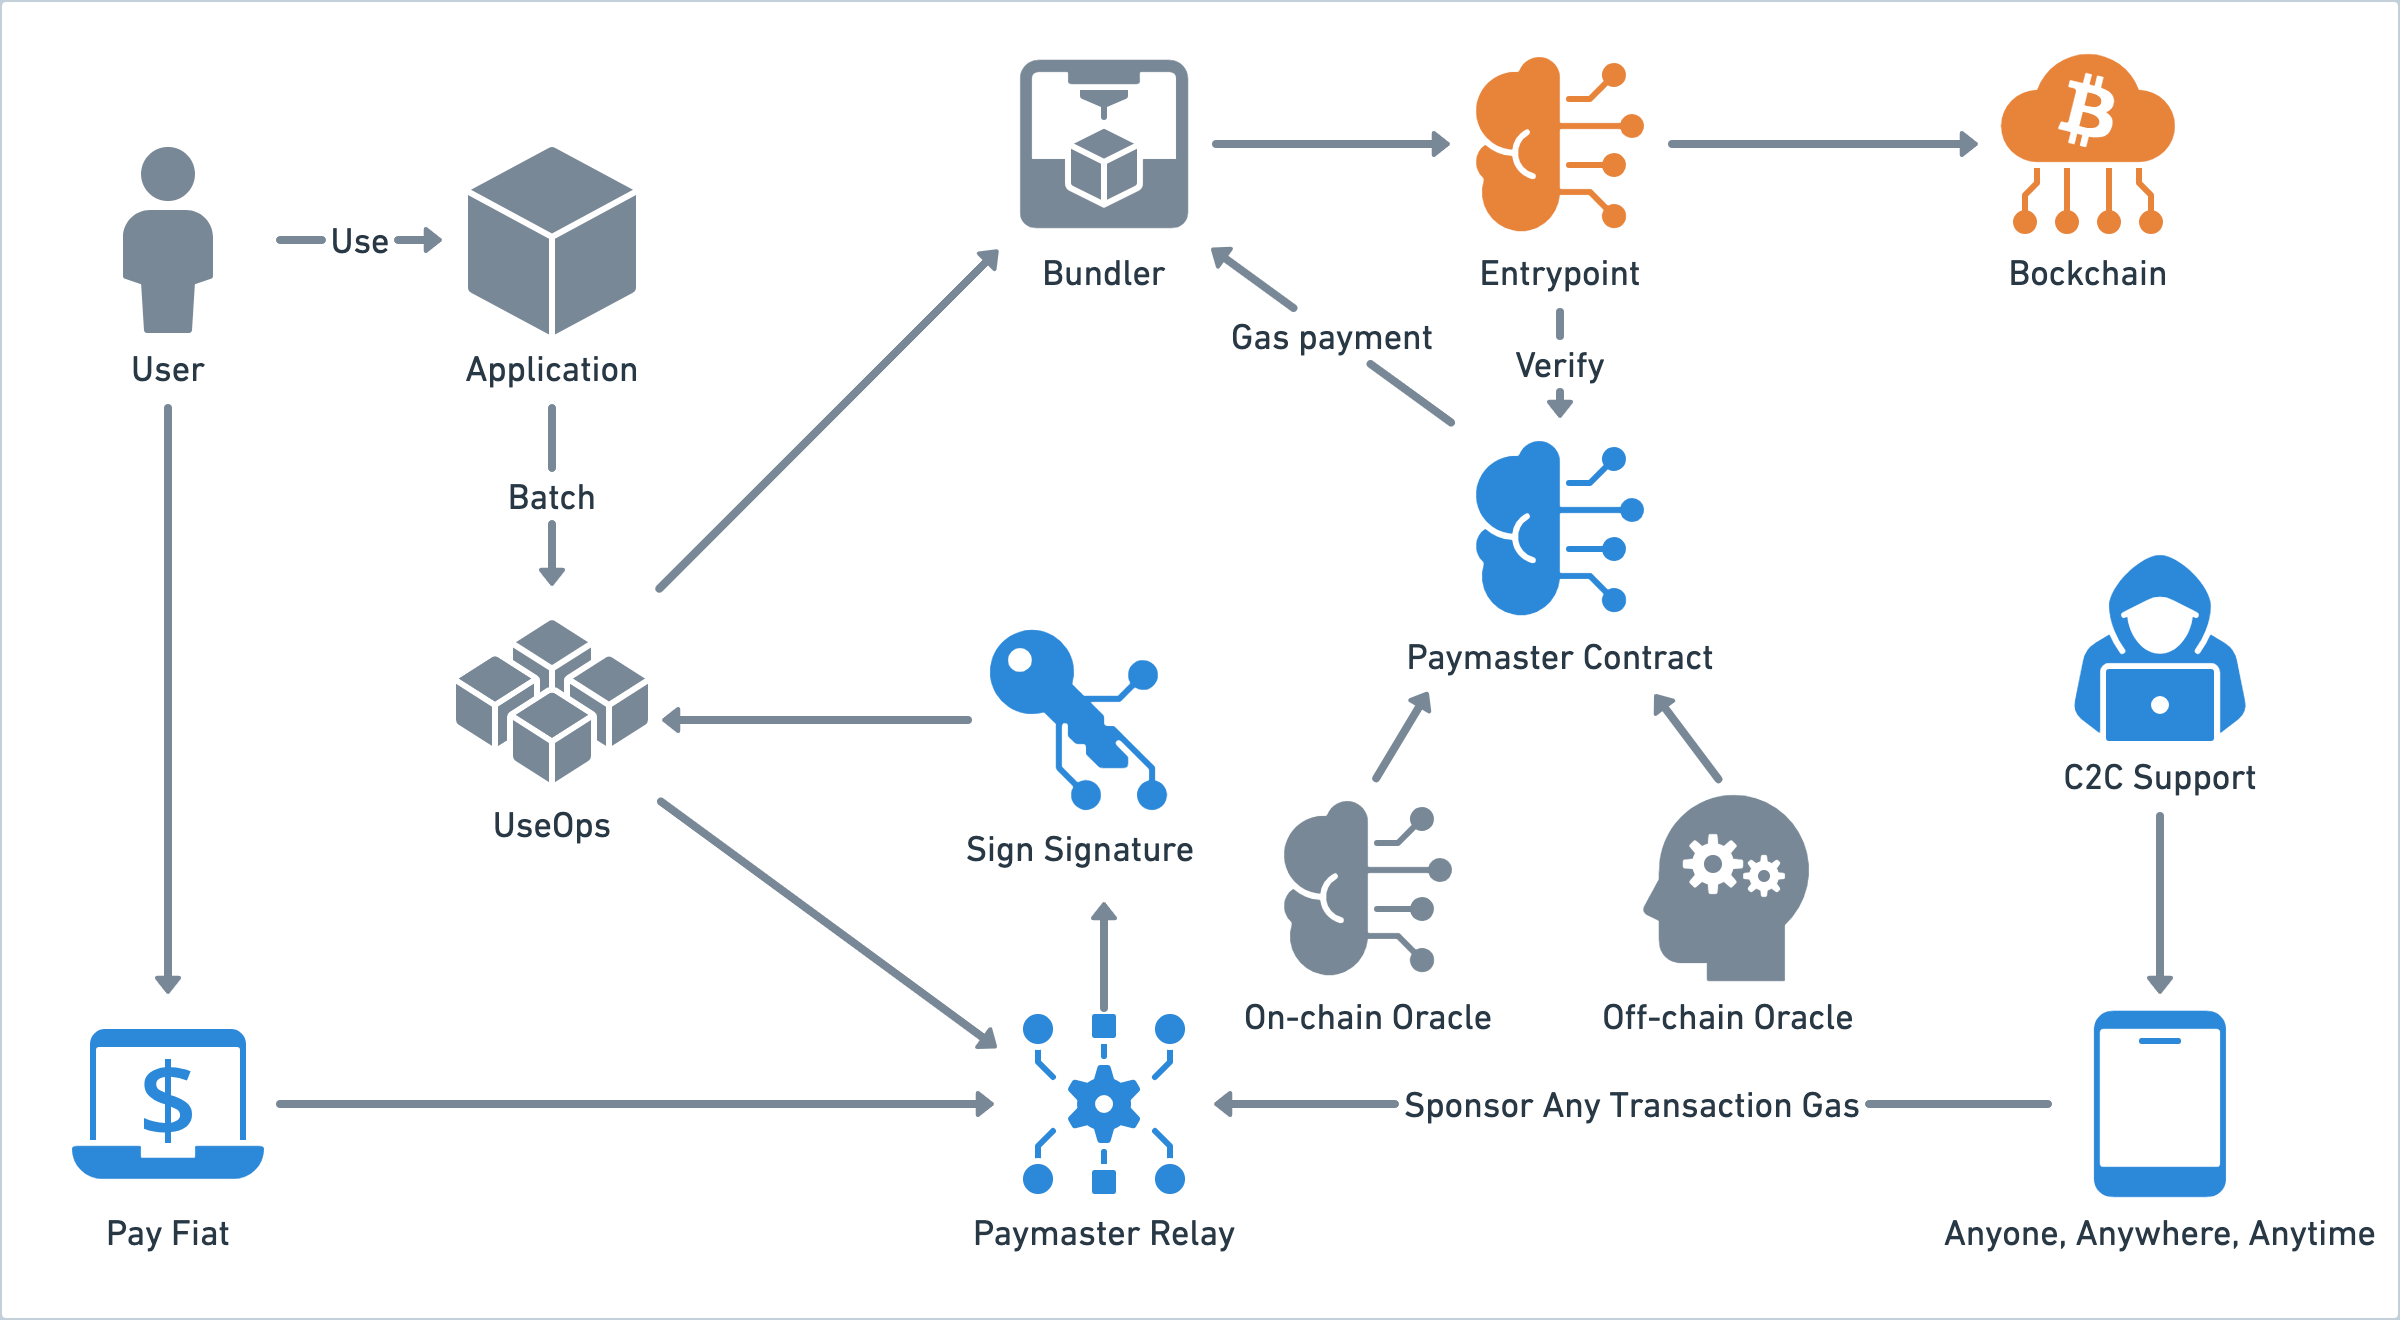
\includegraphics[width=0.75\textwidth]{current-paymaster-solution-figure}
\caption{Current Paymaster Solution Flow in Industry}
\label{fig:current-paymaster-solution}
\end{figure}

\subsubsection{Bad UX: Usability Gap}

From both HCI and TAM perspectives\cite{frohlich2022,shneiderman2010,norman2013,rogers2023,murray2023,preece1994,helander2014,davis1989,maranguni2015}, current systems exhibit numerous characteristics detrimental to user adoption. They often impose a high cognitive load, demonstrate poor usability across multiple dimensions (detailed in Section \ref{subsec:usability-challenges}), involve significant direct and indirect costs, necessitate convoluted multi-step processes, offer a super overall experience, and raise security concerns for average users\cite{frohlich2022}. This poor user experience often stems from the requirement for users to interact with highly abstract concepts lacking clear analogues in their everyday, socially learned experiences, thus failing to align with established mental models\cite{glomann2019}.

\subsubsection{Low Efficiency: Steps and Asset Fragmentation}

The multi-step workflow described in 2.1.2 is inherently inefficient. Each step, from CEX onboarding and KYC delays to cross-chain bridge waiting times and transaction confirmation latency, introduces friction and consumes considerable user time and effort. This inefficiency persists even for experienced users, hindering fluid interaction with dApps\cite{pacheco2023}.

The proliferation of diverse blockchain networks (Layer 1s and Layer 2s) necessitates users holding small balances of different native tokens (e.g., ETH on Ethereum mainnet, ETH on Arbitrum, MATIC on Polygon) simply to pay gas fees on each respective chain. This fragmentation increases user overhead, complicates asset management, and adds significant cumulative costs associated with acquiring and managing these disparate gas tokens \cite{l2fees2024, ultrasoundmoney}.

\subsubsection{Security Risks: Centralized Gas Payment Services (Overview)}

The rise of centralized services offering gas sponsorship (Paymasters) or transaction relaying (Bundlers), often associated with ERC-4337 implementations, introduces a new set of risks that potentially undermine blockchain's core principles. These include security vulnerabilities \cite{liang2023,daian2020}, the potential for transaction manipulation or censorship based on the provider's policies or jurisdiction, and the risk of market monopolies leading to inflated costs and reduced innovation \cite{daian2020}. A detailed analysis follows in Section \ref{subsec:centralized-risks}. It's paradoxical that permissionless accounts, readily created via ECDSA, often necessitate centralized identification and payment methods to acquire gas for initiating decentralized transactions.

\subsection{Usability Challenges in Gas Payment: An HCI Perspective}
\label{subsec:usability-challenges}

The fundamental challenges outlined previously manifest as significant usability barriers when analyzed through the lens of Human-Computer Interaction (HCI)\cite{frohlich2022,saldivar2023,krug2009,glomann2019}. These barriers are particularly pronounced because interacting with gas systems requires users to grasp entirely new, abstract concepts, often without the aid of familiar analogies or metaphors derived from their existing knowledge base.

% Table 5: Usability Challenges in Gas Payments from an HCI Perspective
\begin{table}[htbp]
\centering
\footnotesize
\renewcommand{\arraystretch}{0.9}
\begin{tabularx}{\textwidth}{|p{2.5cm}|X|X|}
\hline
\textbf{HCI Challenge} & \textbf{The Core Problem} & \textbf{Specific Impact on Users} \\
\hline
\textbf{Ease of Learning} & \textbf{Abstract Concepts \& Complex Process:} Users must learn numerous new, non-analogous concepts (e.g., Gas, Gwei, addresses) and master a complex, multi-step workflow. & Extremely steep learning curve, making it difficult for new users to quickly learn and navigate the system effectively. \\
\hline
\textbf{Gulf of Execution} & \textbf{Mismatch Between Intent \& Action:} A huge gap exists between a user's simple intention (e.g., "buy an NFT") and the required system actions (get native tokens, manage keys, set gas). & Users are confused about how to translate their goals into actions, as the process is unfamiliar and disconnected from traditional financial interactions. \\
\hline
\textbf{Gulf of Evaluation} & \textbf{Opaque System State:} Users struggle to understand transaction costs (volatile gas fees), progress (technical hashes), and failure reasons (cryptic errors), making it hard to assess outcomes. & Users feel uncertain about the results of their actions and are unsure how to proceed after a failure due to a lack of clear, understandable feedback. \\
\hline
\textbf{Efficiency Issues} & \textbf{Time-Consuming Workflow:} The entire process, from KYC and fiat on-ramps to bridging and on-chain confirmation, is plagued by delays, creating a slow and cumbersome experience. & Hinders rapid or spontaneous interactions with dApps, leading to a sluggish and inefficient user experience. \\
\hline
\textbf{High Error Rate \& Low Fault Tolerance} & \textbf{Irreversible \& Costly Mistakes:} Simple errors like sending to a wrong address, selecting the wrong network, or setting inadequate gas can lead to permanent fund loss, with no "undo" or robust prevention mechanisms. & The stakes are extremely high for users, where a small mistake can be catastrophic. The system is unforgiving of user error. \\
\hline
\textbf{Memorization Difficulties} & \textbf{Heavy Cognitive Load for Recall:} Users are required to securely memorize/store complex seed phrases, distinguish between cryptic addresses, and recall specific procedures for different chains/dApps. & Places a significant burden on user memory, increasing cognitive load and the likelihood of critical errors. \\
\hline
\textbf{Low User Satisfaction} & \textbf{Poor Overall Experience:} The combination of high cognitive load, inefficiency, and the risk of costly errors leads to widespread user frustration and dissatisfaction. & The fundamentally poor usability of gas payments significantly detracts from a positive user experience, regardless of the dApp's utility. \\
\hline
\textbf{Lack of Supporting Tools} & \textbf{Missing Infrastructure for Developers:} The ecosystem lacks standardized, easy-to-integrate tools for developers to build user-friendly gas solutions, making it costly to create smooth experiences. & dApp developers must either rely on complex external wallet UIs or invest heavily in custom solutions, leading to inconsistent user experiences. \\
\hline
\textbf{High Cognitive Load} & \textbf{Information Overload:} Users must process a massive volume of novel technical concepts (Nonce, MEV, etc.) without intuitive metaphors, consuming significant mental effort. & Learning and performing tasks become exceptionally difficult, leaving users feeling mentally exhausted and hindering deeper engagement with the system. \\
\hline
\textbf{Low Perceived Ease of Use} & \textbf{Negative First Impression:} The initial perception is that blockchain systems are inherently complex, expensive, and insecure, failing to map to users' existing interaction patterns. & This perception acts as a major barrier to trial and adoption, deterring potential users before they even experience the underlying dApp's value. \\
\hline
\end{tabularx}
\caption{Usability Challenges in Gas Payments from an HCI Perspective}
\label{tab:usability-challenges}
\end{table}

\subsection{Risk Analysis of Centralized Gas Payment Services}
\label{subsec:centralized-risks}

While centralized services aim to simplify gas payments, often leveraging ERC-4337 components like Paymasters, they introduce distinct risks stemming from their centralized nature, bring new risk to make blockchain be centralized.

% Table 6: Risk Analysis of Centralized Gas Payment Services
\begin{table}[htbp]
\centering
\footnotesize
\renewcommand{\arraystretch}{0.9}
\begin{tabularx}{\textwidth}{|p{3cm}|X|X|}
\hline
\textbf{Risk Category} & \textbf{Analysis \& Mechanism (The "How" and "Why")} & \textbf{Evidence \& Specific Examples} \\
\hline
\textbf{Economic \& Integration Barriers} & Centralized solutions demand that dApp developers integrate proprietary SDKs and accept service agreements. Furthermore, the underlying ERC-4337 smart contract accounts have a higher base gas cost than standard accounts (EOAs), creating an economic disincentive. & \begin{itemize}[noitemsep,topsep=0pt]
\item High integration costs for developers.
\item Inherent gas overhead of ERC-4337 accounts.
\item \textbf{Source:} [16]
\end{itemize} \\
\hline
\textbf{Transaction Manipulation (MEV)} & Centralized entities like Bundlers and Paymasters gain a privileged view of the transaction flow. This position enables them to reorder, insert, or delay transactions to extract value from users before transactions are confirmed on-chain. & \begin{itemize}[noitemsep,topsep=0pt]
\item \textbf{Practices:} Front-running, sandwich attacks.
\item \textbf{Impact:} Value is extracted from users' trades at their expense.
\item \textbf{Source:} [33]
\end{itemize} \\
\hline
\textbf{Privacy Leakage} & These services become central aggregators of vast amounts of user transaction data. This data, which can be linked to identifiers like IP addresses, creates a single point of failure for user privacy. & \begin{itemize}[noitemsep,topsep=0pt]
\item \textbf{Risks:} Data breaches, data sold to third parties, or use for surveillance.
\item \textbf{Impact:} Reveals user behavior and sensitive financial activity.
\end{itemize} \\
\hline
\textbf{Censorship \& Regulatory Risk} & As centralized entities, these services are subject to jurisdictional laws. They can be compelled to block or censor transactions involving addresses on government sanction lists, undermining the core principle of a permissionless network. & \begin{itemize}[noitemsep,topsep=0pt]
\item \textbf{Example:} Blocking transactions to/from addresses on OFAC's sanction list.
\item \textbf{Irony:} Users must perform KYC/AML on centralized exchanges to fund "permissionless" activities.
\end{itemize} \\
\hline
\textbf{Limited Gas Token Support} & Paymaster services often restrict which tokens are accepted for gas payments, typically favoring large stablecoins or their own platform tokens. This limits user choice and the utility of a project's native token. & \begin{itemize}[noitemsep,topsep=0pt]
\item \textbf{Impact:} Forces users into additional, potentially costly token swaps.
\item \textbf{Hindrance:} Prevents communities from using their own native tokens for network participation.
\end{itemize} \\
\hline
\textbf{Monopoly \& Cost Inflation} & The market for centralized relayers is already showing significant concentration. This leads to a risk of an oligopoly or monopoly where a few dominant players can control the market, dictate terms, and inflate costs over time. & \begin{itemize}[noitemsep,topsep=0pt]
\item \textbf{Long-term Risks:} Increased fees, reduced service quality, and stifled innovation.
\item \textbf{Data:} Market concentration is shown by Figure \ref{fig:centralized-paymaster-monopoly} (data from BundleBear).
\item \textbf{Source:} [6]
\end{itemize} \\
\hline
\end{tabularx}
\caption{Risk Analysis of Centralized Gas Payment Services}
\label{tab:risk-analysis}
\end{table}

\begin{figure}[htbp]
\centering
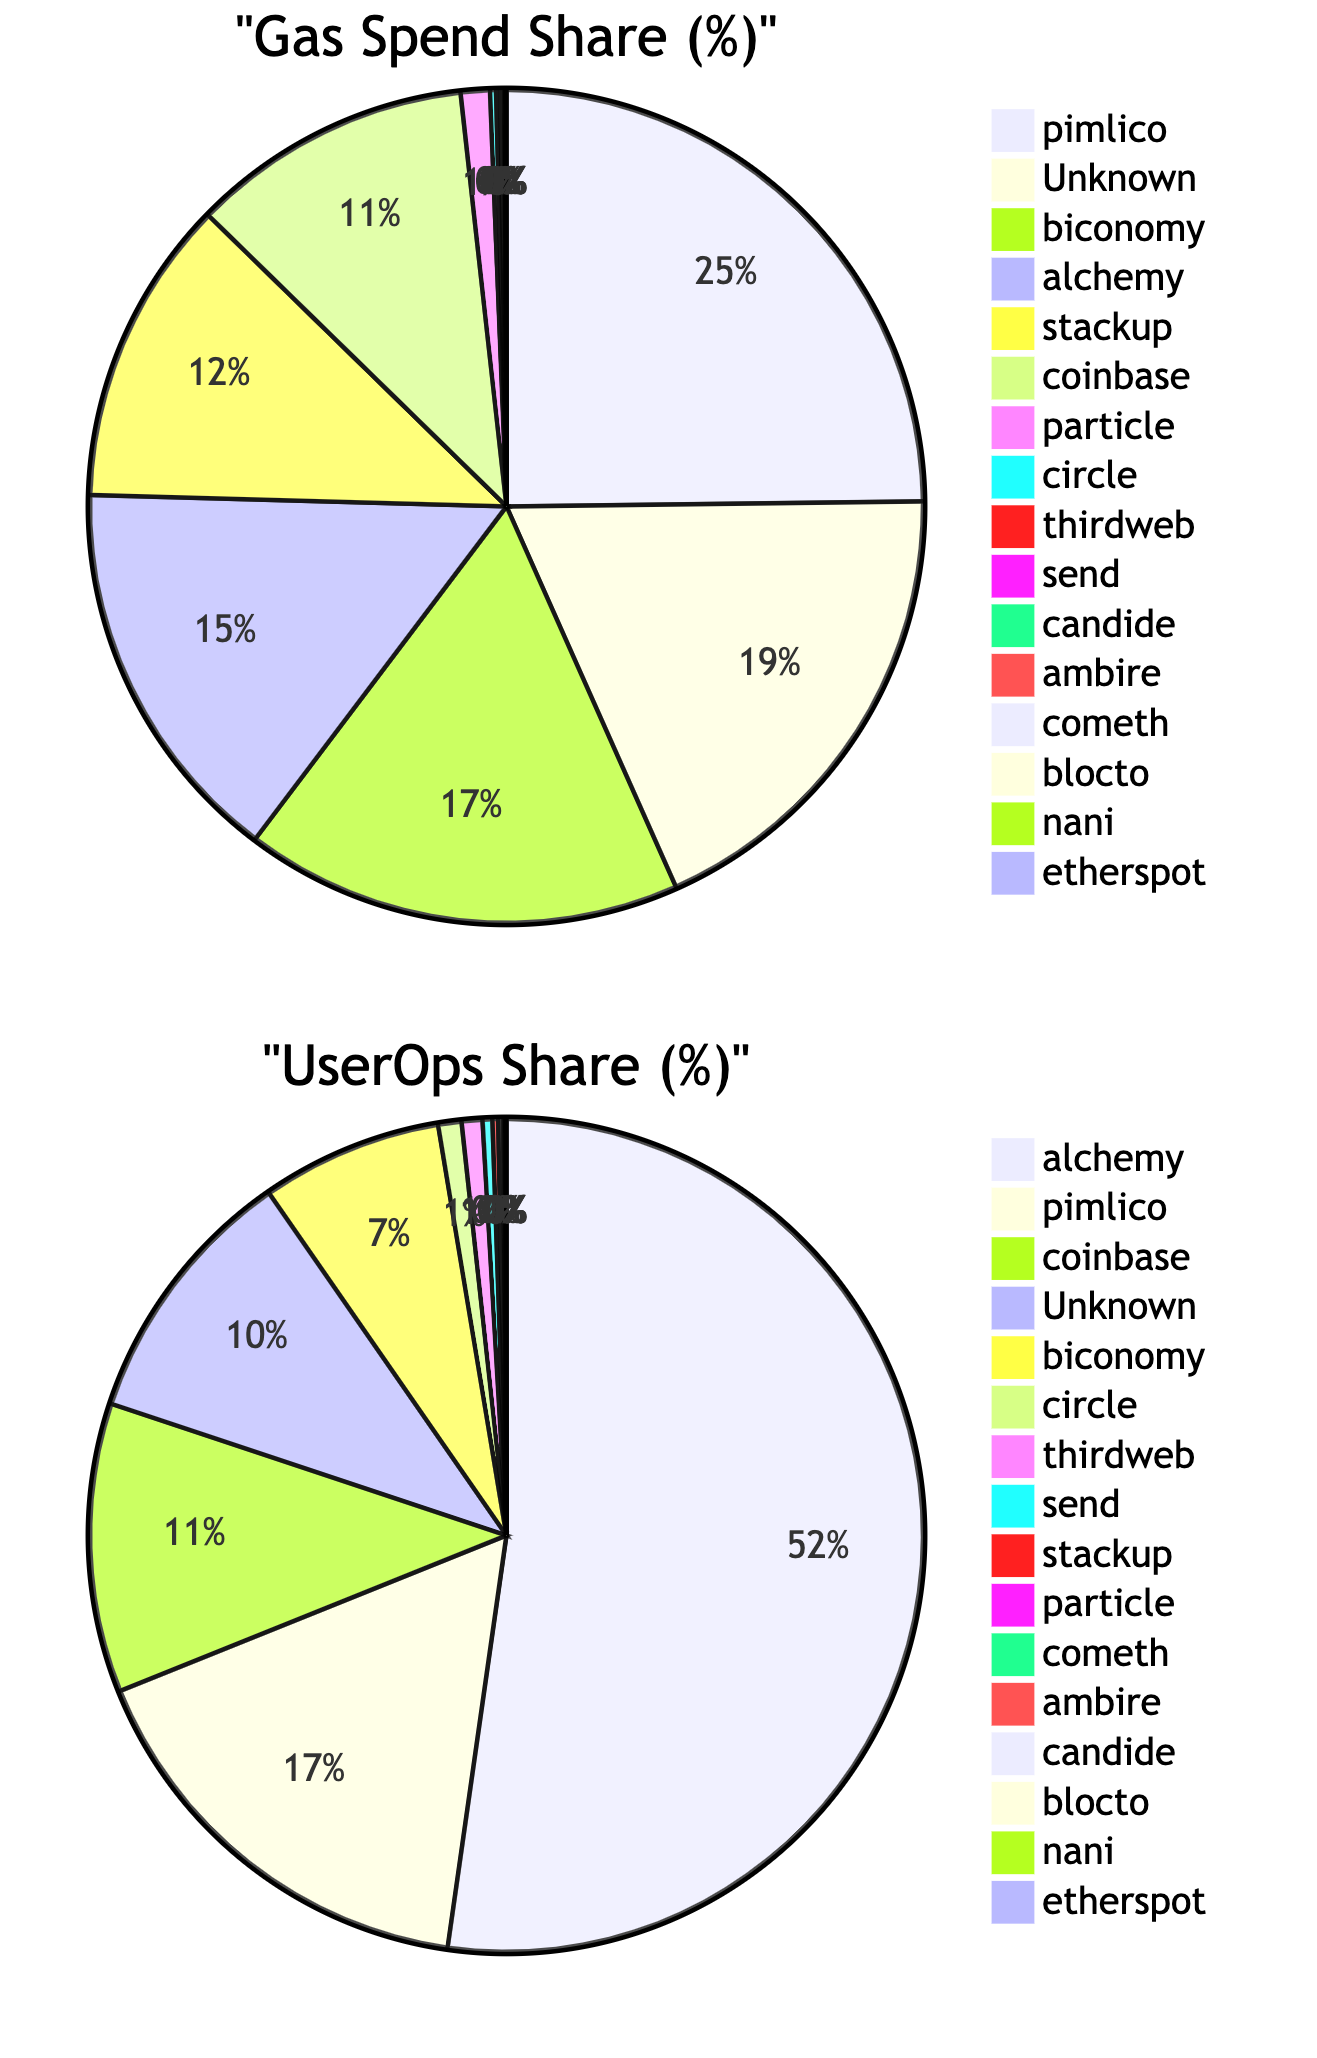
\includegraphics[width=0.75\textwidth]{centralized-paymaster-monopoly-figure}
\caption{Centralized Paymaster Market Monopoly Graph, data source: BundlBear}
\label{fig:centralized-paymaster-monopoly}
\end{figure}

\section{The Proposed System Overview: SuperPaymaster}
\label{sec:proposed-system}

Addressing the multifaceted challenges detailed in Section \ref{sec:analysis} requires a paradigm shift from centralized or simplistic gas payment solutions towards a decentralized, user-centric, and competitive system, one designed by leveraging familiar user paradigms to abstract technical complexity. This section introduces SuperPaymaster, a novel system designed to achieve this vision. We first outline the critical requirements for such a system, then provide an overview of SuperPaymaster's architecture and actors, delve into its core components including the foundational Standardized Decentralized Service System (SDSS), and finally, detail its operational workflows from both system and user perspectives.

\subsection{Requirements Specification for a Decentralized Gas Payment System}
\label{subsec:requirements}

To achieve the vision of a truly decentralized, user-centric, and competitive gas payment system, we have identified three core requirements that serve as foundational principles for SuperPaymaster's design and implementation.

% Table 8: Core Requirements Table for the SuperPaymaster System
\begin{table}[htbp]
\centering
\footnotesize
\renewcommand{\arraystretch}{0.9}
\begin{tabularx}{\textwidth}{|p{3cm}|X|X|}
\hline
\textbf{General Requirement} & \textbf{Core Goal (Why this is needed)} & \textbf{Key Components \& Mechanisms (How it's achieved)} \\
\hline
\textbf{1. Robustness \& Trustworthiness} & To build a secure, reliable, and privacy-preserving foundation that users and dApps can depend on, ensuring the integrity of all operations. & \begin{itemize}[noitemsep,topsep=0pt]
\item \textbf{Security:} Protect user funds and data with strong authentication (e.g., D2FA) and defense against on-chain attacks.
\item \textbf{Privacy:} Minimize data exposure and prevent surveillance, potentially using technologies like TEEs.
\item \textbf{Availability:} Guarantee consistent uptime and fault tolerance through a decentralized network of redundant service nodes.
\end{itemize} \\
\hline
\textbf{2. User-Centricity \& Economic Viability} & To abstract all technical complexity, making gas payments invisible, effortless, and highly affordable for the end-user, thereby creating a Web2-like experience. & \begin{itemize}[noitemsep,topsep=0pt]
\item \textbf{Usability:} Lower the learning curve by leveraging familiar mental models like "prepaid cards" or "loyalty points" (via OpenCards/NFTs).
\item \textbf{Cost-Effectiveness:} Drive down costs with competitive quoting and enable zero/negative cost for users via community points (OpenPNTs).
\item \textbf{Efficiency:} Ensure swift and streamlined transaction processing to deliver a seamless user experience.
\end{itemize} \\
\hline
\textbf{3. Decentralization \& Open Competition} & To create a fair, open, and permissionless market that prevents censorship and monopolies, ensuring long-term system health, innovation, and community empowerment. & \begin{itemize}[noitemsep,topsep=0pt]
\item \textbf{Competitiveness:} Foster a dynamic market among service providers with reputation systems and competitive quoting to ensure fair pricing.
\item \textbf{Openness:} Build on open-source principles where anyone can participate as a user, developer, or service node operator.
\item \textbf{Permissionless:} Allow any community to issue its own gas tokens and any node to freely join the network without central approval.
\end{itemize} \\
\hline
\end{tabularx}
\caption{Core Requirements Table for the SuperPaymaster System}
\label{tab:core-requirements}
\end{table}

\subsection{Overview of the SuperPaymaster System}
\label{subsec:system-overview}

SuperPaymaster is proposed as a decentralized gas payment (sponsorship) system built upon the ERC-4337 standard and leveraging a novel Standardized Decentralized Service System (SDSS) architecture. Its core objective is to create an open, competitive, and resilient marketplace for gas sponsorship, addressing the cost, usability, efficiency, and centralization issues prevalent in existing solutions. Key motivations include providing a single, consistent Paymaster address across chains for developer convenience and unifying the staking mechanism for all participating sponsors (LPs/Nodes) to enhance overall system trust and reliability. It facilitates various user-friendly payment models addressing the cost and usability issues mentioned above, all managed within a decentralized framework that utilizes relatable concepts like 'Gas Cards' to simplify user interaction.

\begin{figure}[htbp]
\centering
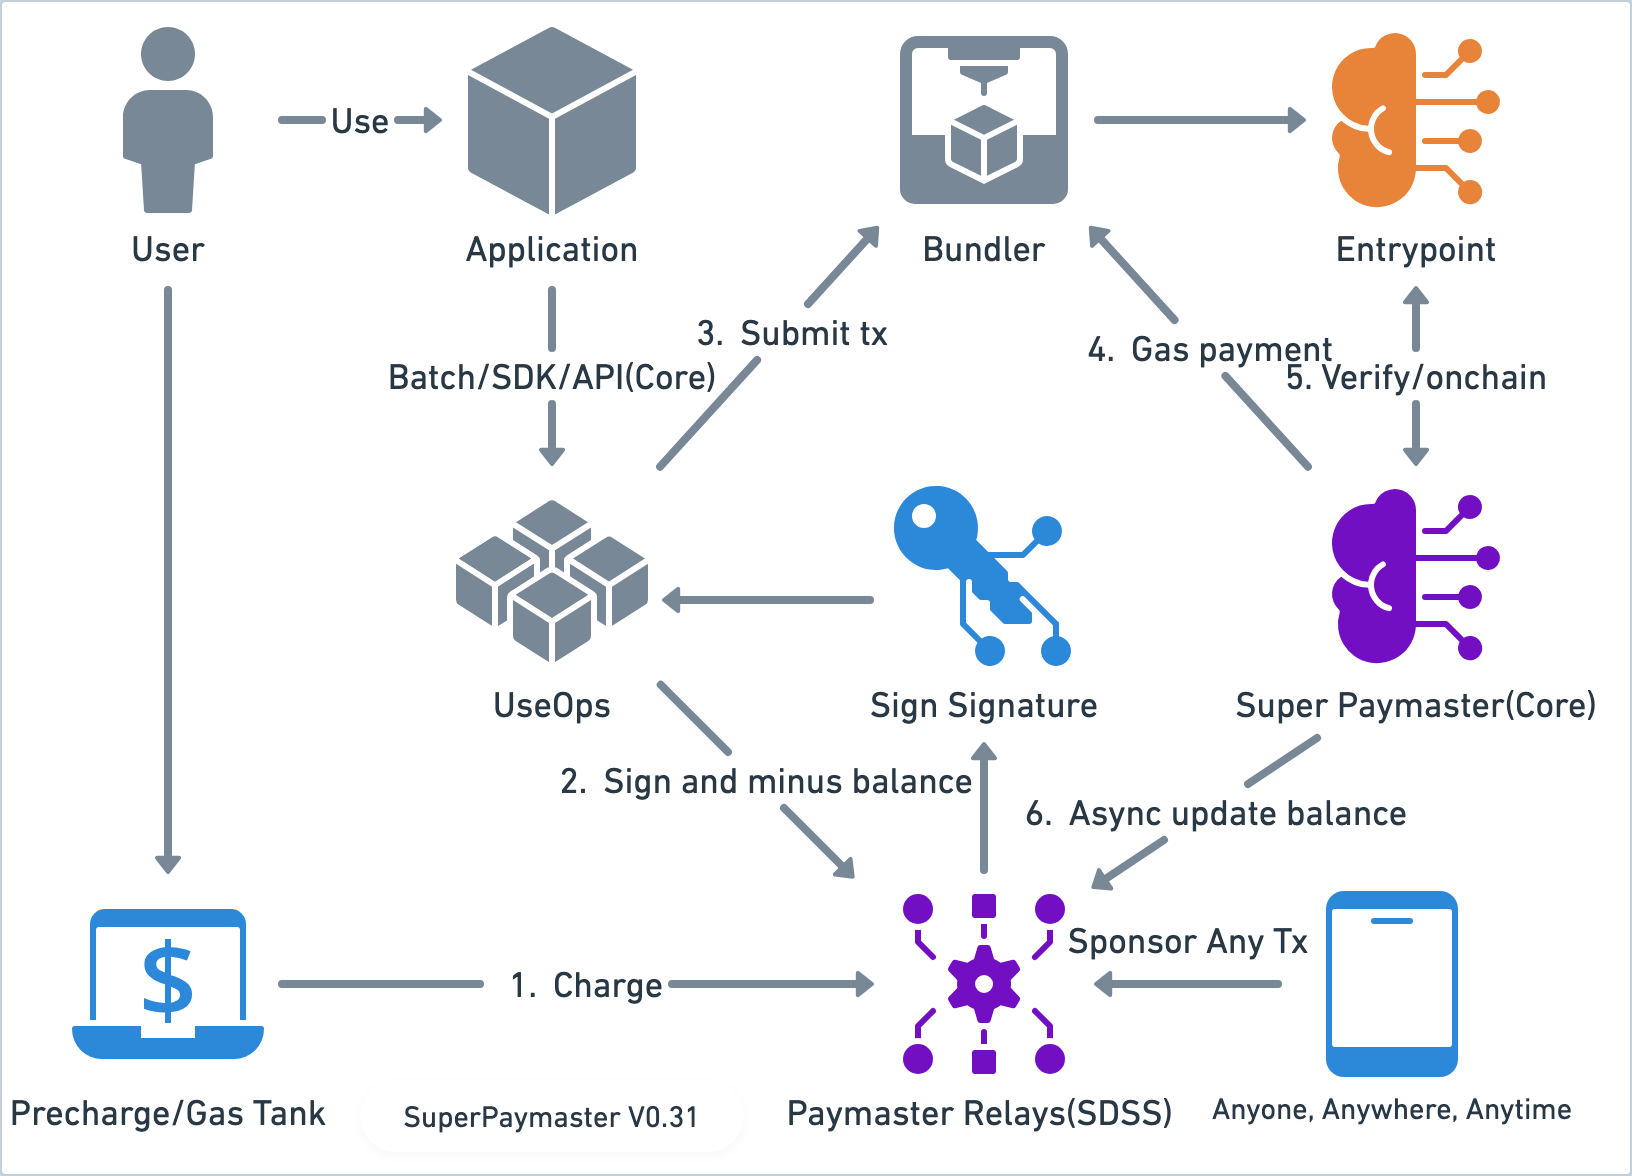
\includegraphics[width=0.7\textwidth]{superpaymaster-system-flow-figure}
\caption{SuperPaymaster System Flow Overview}
\label{fig:superpaymaster-system-flow}
\end{figure}

\subsection{Involved Actors and Roles}
\label{subsec:actors-roles}

The SuperPaymaster system involves several key actors based on ERC4337 solution\cite{buterin2021}:

\textbf{End Users} Individuals interacting with dApps who require gas payments for their transactions. They benefit from simplified processes, lower costs, and enhanced security via systems like AirAccount.

\textbf{dApps (Decentralized Applications)} Applications integrating SuperPaymaster (via SDSS APIs) to offer seamless gas payment experiences to their users.

\textbf{Communities} Groups or organizations that may issue their own ERC-20 tokens (OpenPNTs) usable for gas payments within the SuperPaymaster network via OpenCards, fostering community engagement.

\textbf{Node Operators (Paymaster / Gas Sponsors / LPs)} Entities running the SuperPaymaster service nodes. They register within the SDSS, stake collateral in the SuperPaymaster contract, listen for gas sponsorship requests, provide quotes, sign UserOperations, and facilitate gas payments. They are incentivized through service fees and reputation gains. Multiple node types (N1, N2, N3 with varying capabilities like TEE) may exist.

\textbf{Bundlers / RPC Providers} Entities responsible for bundling UserOperations (containing Paymaster data) into transactions and submitting them to the blockchain's transaction pool (or directly to block builders under future proposals like RIP-7560\cite{rip7560}).

\textbf{On-Chain Contracts} We use Superpaymaster contract to verify off-chain signature and handle the gas sponsorship and payment. All transaction rely on official EntryPoint contract to verify, launch and guarantee basic security from EIP-4337 team.

\textbf{Third-Party Swap Services (Optional)} Services that may be integrated to facilitate real-time conversion between various ERC-20 tokens and the native gas token (e.g., ETH) if required by the Paymaster node.

\subsection{SDSS (Standardized Decentralized Service System) Overview}
\label{subsec:sdss-overview}

SDSS serves as the foundational communication and discovery layer for decentralized services for the SuperPaymaster system. It aims to provide a secure, transparent, and user-friendly architecture for basic decentralized computing services, moving beyond reliance on traditional centralized cloud infrastructure. Its core components facilitate the discovery and interaction with permissionlessly operated service nodes.

(Note: Detailed SDSS components are elaborated in 3.5.2)

\subsection{The infrastructure of SuperPaymaster System}
\label{subsec:key-components}

SuperPaymaster integrates several key technological and economic components. These components interact to implement the core functionalities and realize the system's design philosophy of mapping complex blockchain operations onto more familiar user experiences.

\subsubsection{SuperPaymaster Core}

We build SuperPaymaster based on ERC4337, so there are 4 parts:

\begin{enumerate}
\item SuperPaymaster contract: stake the ETH and verify the signature, pay the gas sponsorship.
\item SuperPaymaster relay server: handle the user operation and sign a signature before or after deduce your ERC20 token balance.
\item SuperPaymaster ENS API: response to some quota and routing services directly or push to pool timely.
\item SuperPaymaster client/dApps SDK: help developers to initiate the user operation and submit it to bunlder after get the gas sponsorship signature from SuperPaymaster server.
\end{enumerate}

\subsubsection{Standardized Decentralized Service System (SDSS) / DePIN}

The Standardized Decentralized Service System (SDSS), also conceptualized as a Decentralized Physical Infrastructure Network (DePIN), establishes a core framework for decentralized services. It employs a multi-tiered node architecture, facilitated by a Software Development Kit (SDK), enabling permissionless participation where any entity can operate nodes for self-service or service provision.

\begin{enumerate}
\item \textbf{Node Architecture:}
   \begin{itemize}
   \item \textbf{N0 (Client Node):} Cross-platform client applications (developed with Tauri+Node.js) that access services provided by N1-N3 nodes.
   \item \textbf{N1 (Foundation Service Node):} Provides static file hosting and Ethereum Name Service (ENS) resolution API services.
   \item \textbf{N2 (Secure Compute Node):} Offers TEE (Trusted Execution Environment) and hardware wallet services, leveraging ARM-based platforms (e.g., Raspberry Pi 5B).
   \item \textbf{N3 (Application Service Node):} Runs containerized services (e.g., Dockerized Supabase instances) for broader application support.
   \end{itemize}

\item \textbf{Decentralized Service Discovery and Registration:} This mechanism underpins the dynamic operation of the SDSS:
   \begin{itemize}
   \item \textbf{ENS Registry for Service Discovery:} Leverages the Ethereum Name Service (ENS) for human-readable naming (e.g., \texttt{node.ethpaymaster.eth}) and robust service endpoint resolution. Nodes register API endpoints and metadata within ENS records, creating a decentralized alternative to centralized registries.
   \item \textbf{Node Registration Mechanism:} Provides a secure, potentially pseudonymous (via blockchain address) on-chain registry. Nodes register their service capabilities, API endpoints (linked via ENS), and public keys. This process involves staking collateral (e.g., into a SuperPaymaster contract) to ensure accountability and security.
   \item \textbf{Dynamic Routing and Discovery:} Client applications (N0 or dApps) dynamically locate suitable API service nodes by querying the ENS-based registry (e.g., \texttt{api.aastar.eth}) or through client-side cached lists. This enables self-maintenance of service records, facilitates failover, and allows for node selection based on criteria such as reputation or network proximity.
   \end{itemize}
\end{enumerate}

\begin{figure}[htbp]
\centering
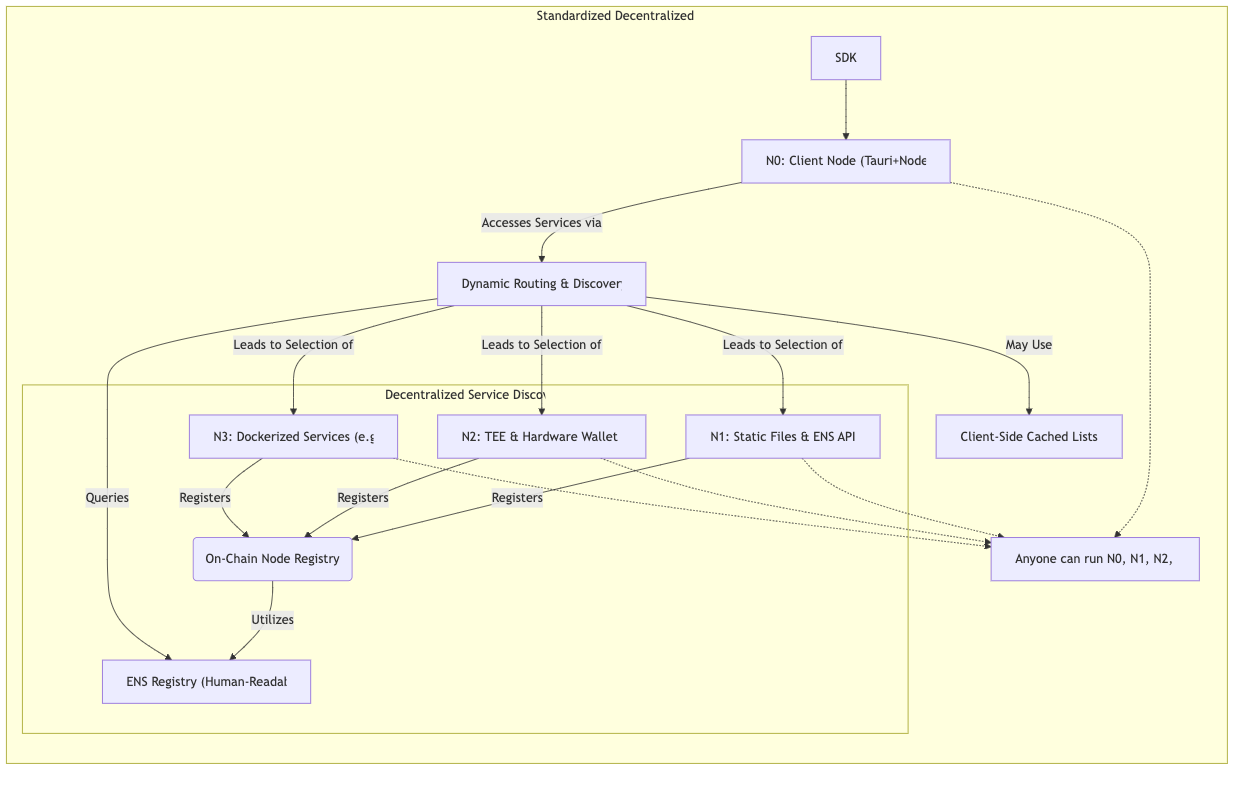
\includegraphics[width=0.8\textwidth]{sdss-depin-architecture-figure}
\caption{SDSS DePIN Architecture}
\label{fig:sdss-depin-architecture}
\end{figure}

\subsubsection{Competitive Quoting Mechanism}

Instead of relying on a single provider's price, dApps can query multiple registered SuperPaymaster nodes (discovered via SDSS) for gas sponsorship quotes for a specific transaction. The dApp can then select the most favorable quote (e.g., lowest cost, highest reputation node, specific ERC20 token), fostering price competition and preventing monopolies. They(dApps) can fetch by a single API from SDSS service to get multiple quotes and access API URLs. All quotes will be updated by SDSS.

\subsubsection{Self-Custodial AirAccount Integration: Secure and User-Centric Account Management}

This component leverages the AirAccount system to provide robust and user-centric account management. All user operations are securely authorized via AirAccount, employing a dual-factor approach:

\begin{enumerate}
\item \textbf{Biometric Authentication (D2FA):} Utilizes device-based biometrics (e.g., fingerprint via Secure Enclave/TEE, FIDO2/Passkey standards) for transaction signing. This serves as a decentralized second-factor authentication (D2FA), markedly enhancing security beyond conventional private key models while improving usability through intuitive actions like "Just press fingerprint."
\item \textbf{TEE-Secured Private Keys:} Private keys are cryptographically secured within a Trusted Execution Environment (TEE), operating under pre-defined rules to govern their usage.
\end{enumerate}

On-chain, the integrity of every transaction is verified by the smart contract account using BLS12-381 (compliant with EIP-2537) and secp256k1/ECDSA (compliant with ERC4337/EIP-1271) cryptographic algorithms.

Furthermore, this integration confers the inherent advantages of smart contract accounts managed by AirAccount, such as social recovery mechanisms ("moving house"), configurable spending limits, session key management, and the potential for automated will execution features.

\begin{figure}[htbp]
\centering
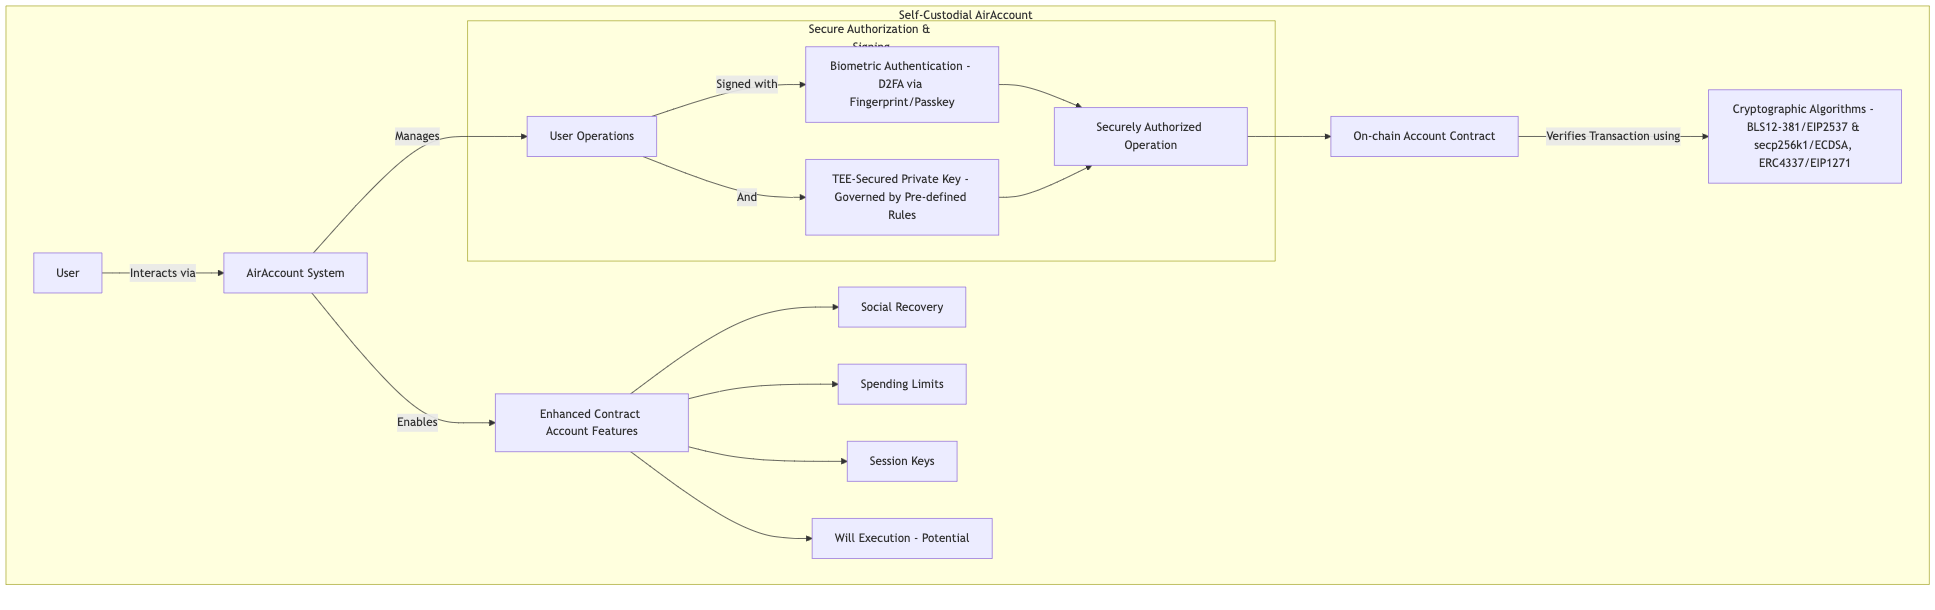
\includegraphics[width=0.8\textwidth]{airaccount-integration-figure}
\caption{Self-Custodial AirAccount Integration}
\label{fig:airaccount-integration}
\end{figure}

\subsubsection{Open Community Mode: Flexible Gas Payment \& Community Empowerment}

The Open Community Mode introduces a flexible framework for on-chain gas payment, empowering communities and users through tangible social and economic constructs. This mode allows communities to operate permissionless Community Nodes, offering guidance and gas sponsorship options to users. It comprises three synergistically integrated components designed to simplify blockchain interactions and reduce cognitive load associated with gas fees.

\begin{enumerate}
\item \textbf{Permissionless Community Tokens (OpenPNTs):} This mechanism enables any community to issue its own ERC20-compliant tokens (PNTs). Configured SuperPaymaster nodes accept these PNTs for gas payments, fostering and incentivizing community-specific activities. An extension of ERC20, EIP-777, is utilized for efficient token balance deduction.
\item \textbf{NFT-based Gas Cards (OpenCards):} Leveraging Soul Bound Tokens (SBT) and Non-Fungible Tokens (NFT) (ERC-721/EIP-6551 compatible), this component implements a 'Gas Card' metaphor based on familiar prepaid card mental models. It automatically recognizes identity and facilitates gas payments, providing cardholders with automatic gas deductions (using PNTs or predefined limits) for a seamless "gasless" experience. This approach mitigates the complexity of blockchain interactions, significantly reducing cognitive load and enhancing Perceived Ease of Use (PEOU).
\item \textbf{Task-for-Points Mechanism:} This feature allows users to earn community PNTs by engaging in designated tasks, such as social promotion or content creation. The earned PNTs can subsequently be utilized via OpenCards to cover gas fees, potentially leading to a net-zero or even negative cost for gas transactions.
\end{enumerate}

\begin{figure}[htbp]
\centering
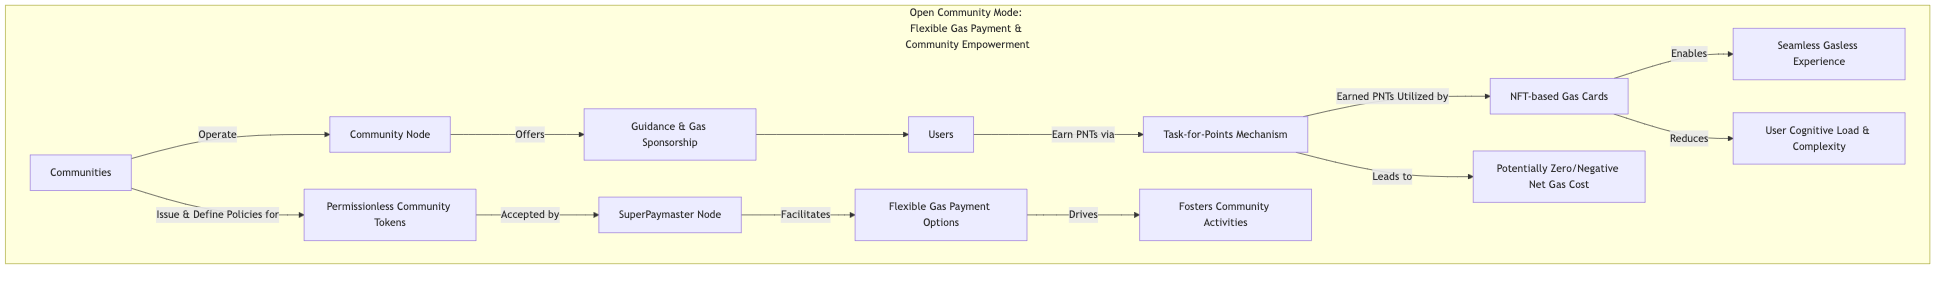
\includegraphics[width=0.8\textwidth]{open-community-mode-figure}
\caption{Open Community Mode: Flexible Gas Payment \& Community Empowerment}
\label{fig:open-community-mode}
\end{figure}

\subsection{Core Gas Sponsorship Workflow (System Perspective)}
\label{subsec:gas-sponsorship-workflow}

The following steps outline the typical process flow when a transaction is sponsored via SuperPaymaster:

Step 1: User Account Registration: User registers/logs in via AirAccount (new or bound EOA).

Step 2: Transaction Construction \& Encryption: User interacts with a dApp, generating transaction data (UserOperation). AirAccount (using fingerprint/passkey) signs the UserOperation.

Step 3: Gas Price Quoting via SDSS: The dApp (or user's wallet/AirAccount backend) uses SDSS (via ENS lookup) to discover available SuperPaymaster nodes and requests gas sponsorship quotes for the UserOperation.

Step 4: Paymaster Selection \& Signature Acquisition: The dApp selects the best quote (based on price, reputation) and requests a Paymaster signature from the chosen node for the UserOperation. The node verifies its ability to sponsor (e.g., checks internal limits, user's OpenCard status/PNT balance if applicable) and provides the signature.

Step 5: Transaction Submission: The dApp/wallet submits the UserOperation (now including the Paymaster signature and data) to a Bundler or directly to an RPC endpoint supporting ERC-4337 (or future AA standards like EIP-7560).

Step 6: On-Chain Verification: The Bundler includes the UserOperation in a bundle transaction sent to the global EntryPoint contract. The EntryPoint verifies the UserOperation, including calling the specified SuperPaymaster contract to validate the Paymaster signature and ensure sufficient deposit/stake exists. AirAccount's signature might also be verified on-chain if needed.

Step 7: Pre-Payment Actions (within Paymaster validatePaymasterUserOp): The SuperPaymaster contract, during validation, checks the sponsoring node's stake and potentially locks funds or deducts pre-paid balance (e.g., from OpenCard associated PNTs). It may need to consult an oracle for real-time token prices if accepting non-native tokens.

Step 8: Contract Execution: If validation succeeds, the EntryPoint executes the core logic of the UserOperation (e.g., token transfer, NFT claim).

Step 9: Post-Payment Actions (within Paymaster postOp): After execution, the EntryPoint calls the SuperPaymaster contract's postOp function. This function handles the actual gas payment reconciliation: paying the Bundler/EntryPoint, potentially refunding excess gas pre-payment to the user/node, updating off-chain account balances, and logging data for reputation calculation.

Step 10: Transaction Confirmation: The Bundler's transaction containing the UserOperation bundle is included in a block and finalized on the blockchain. A transaction hash/receipt is returned.

Step 11: Post-Pay Settlement (Node Level): The sponsoring SuperPaymaster node performs its internal post-transaction accounting, potentially billing users for post-paid services or updating internal ledgers.

A sequence diagram illustrating

\begin{figure}[htbp]
\centering
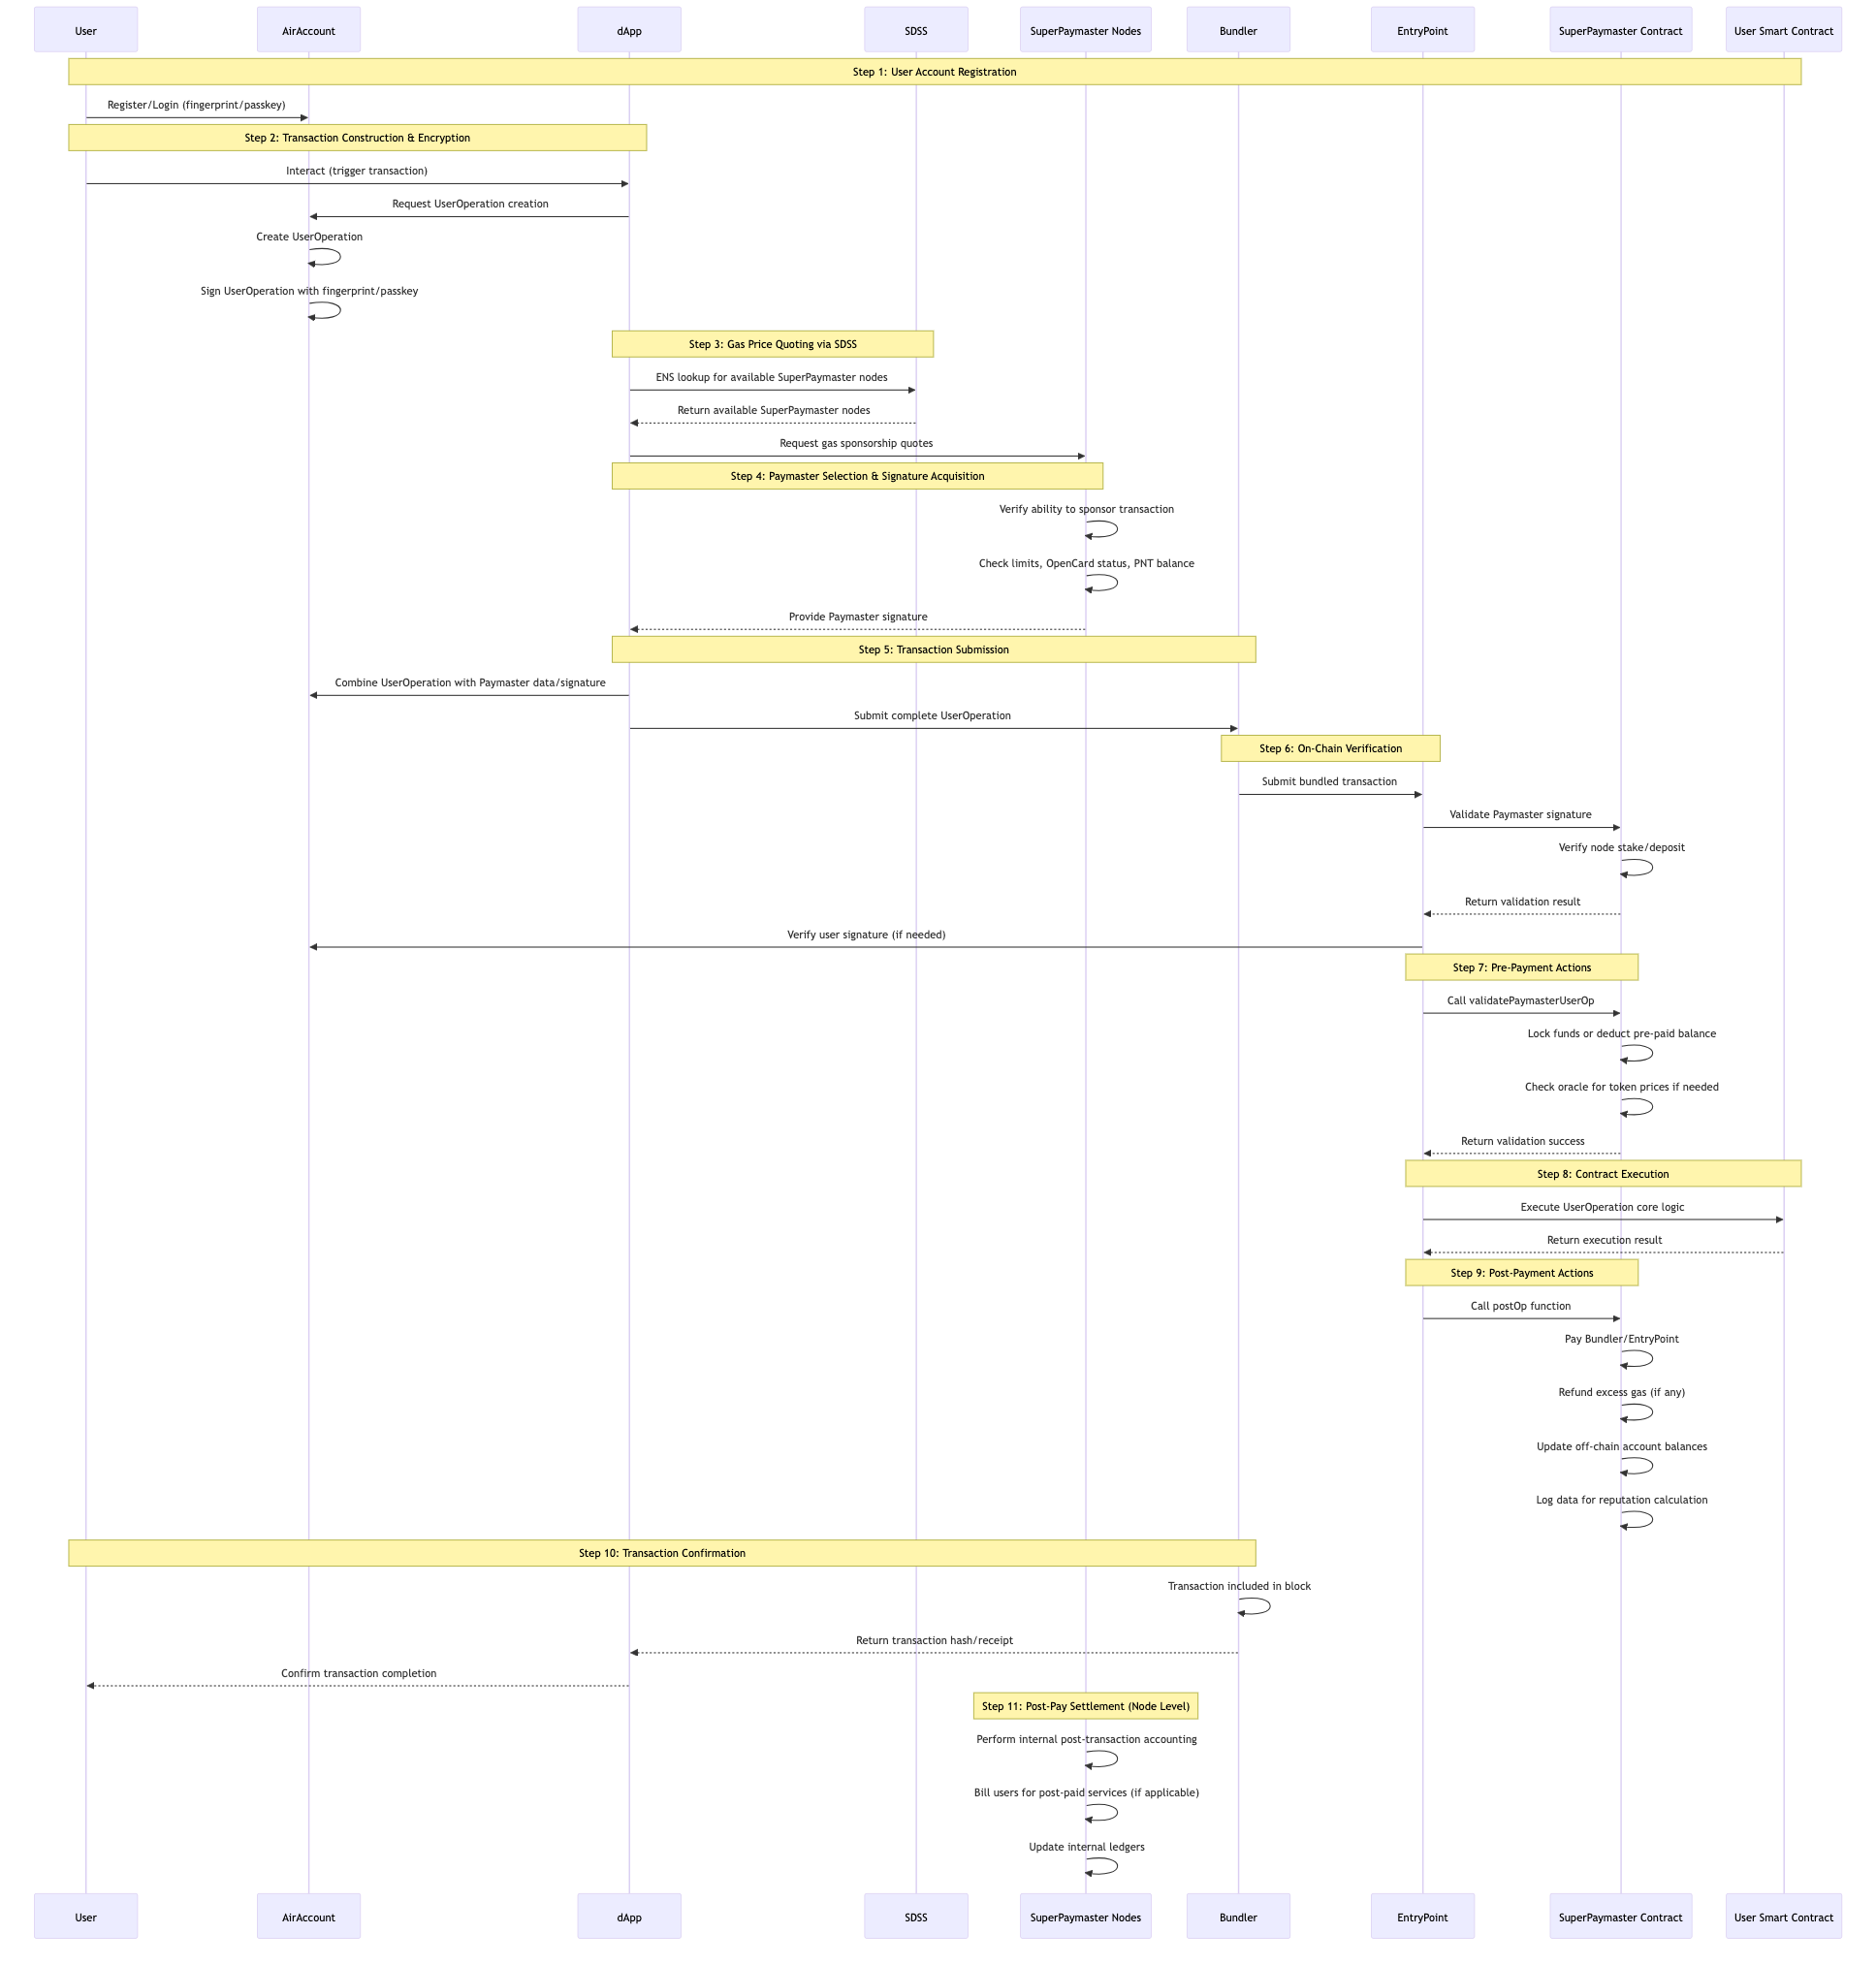
\includegraphics[width=0.9\textwidth]{superpaymaster-flow-sequence-figure}
\caption{SuperPaymaster Flow}
\label{fig:superpaymaster-flow-sequence}
\end{figure}

\subsection{Typical User Interaction Workflow (User Perspective)}
\label{subsec:user-interaction-workflow}

From the end-user's viewpoint, the process is significantly simplified:

Step 1: Accessing Integrated dApp: User visits a dApp that has integrated SuperPaymaster and AirAccount.

Step 2: Account Registration/Login: User logs in or registers using their familiar Web2 method (Google/Email via Passkey/Fingerprint) or by connecting an existing EOA (verified via signature) through the AirAccount interface.

Step 3: Receiving Community NFT/Points (Scenario): Upon joining a community via the dApp, the user might automatically receive an OpenCard NFT representing a gas allowance or initial OpenPNTs balance.

Step 4: Earning Points (Optional): User participates in community activities (e.g., sharing content, completing tasks) and earns OpenPNTs credited to their account/OpenCard.

Step 5: Initiating Transaction: User interacts with the dApp as intended (e.g., clicks "Mint NFT," "Transfer Tokens," "Buy Item").

Step 6: Seamless Gas Payment: The underlying SuperPaymaster system handles the gas payment. If the user holds a valid OpenCard with sufficient PNTs/allowance, the gas fee is automatically deducted or covered without requiring user confirmation or interaction with native tokens. The experience feels "gasless."

Step 7: Viewing Transaction Records: User receives confirmation of the successful transaction within the dApp, similar to a Web2 purchase confirmation. They can view details like transaction ID and status.

Step 8: Checking Balances and History: User can check their OpenPNTs balance, OpenCard status, and transaction history (including gas cost savings estimations) within their AirAccount interface or the dApp.

\begin{figure}[htbp]
\centering
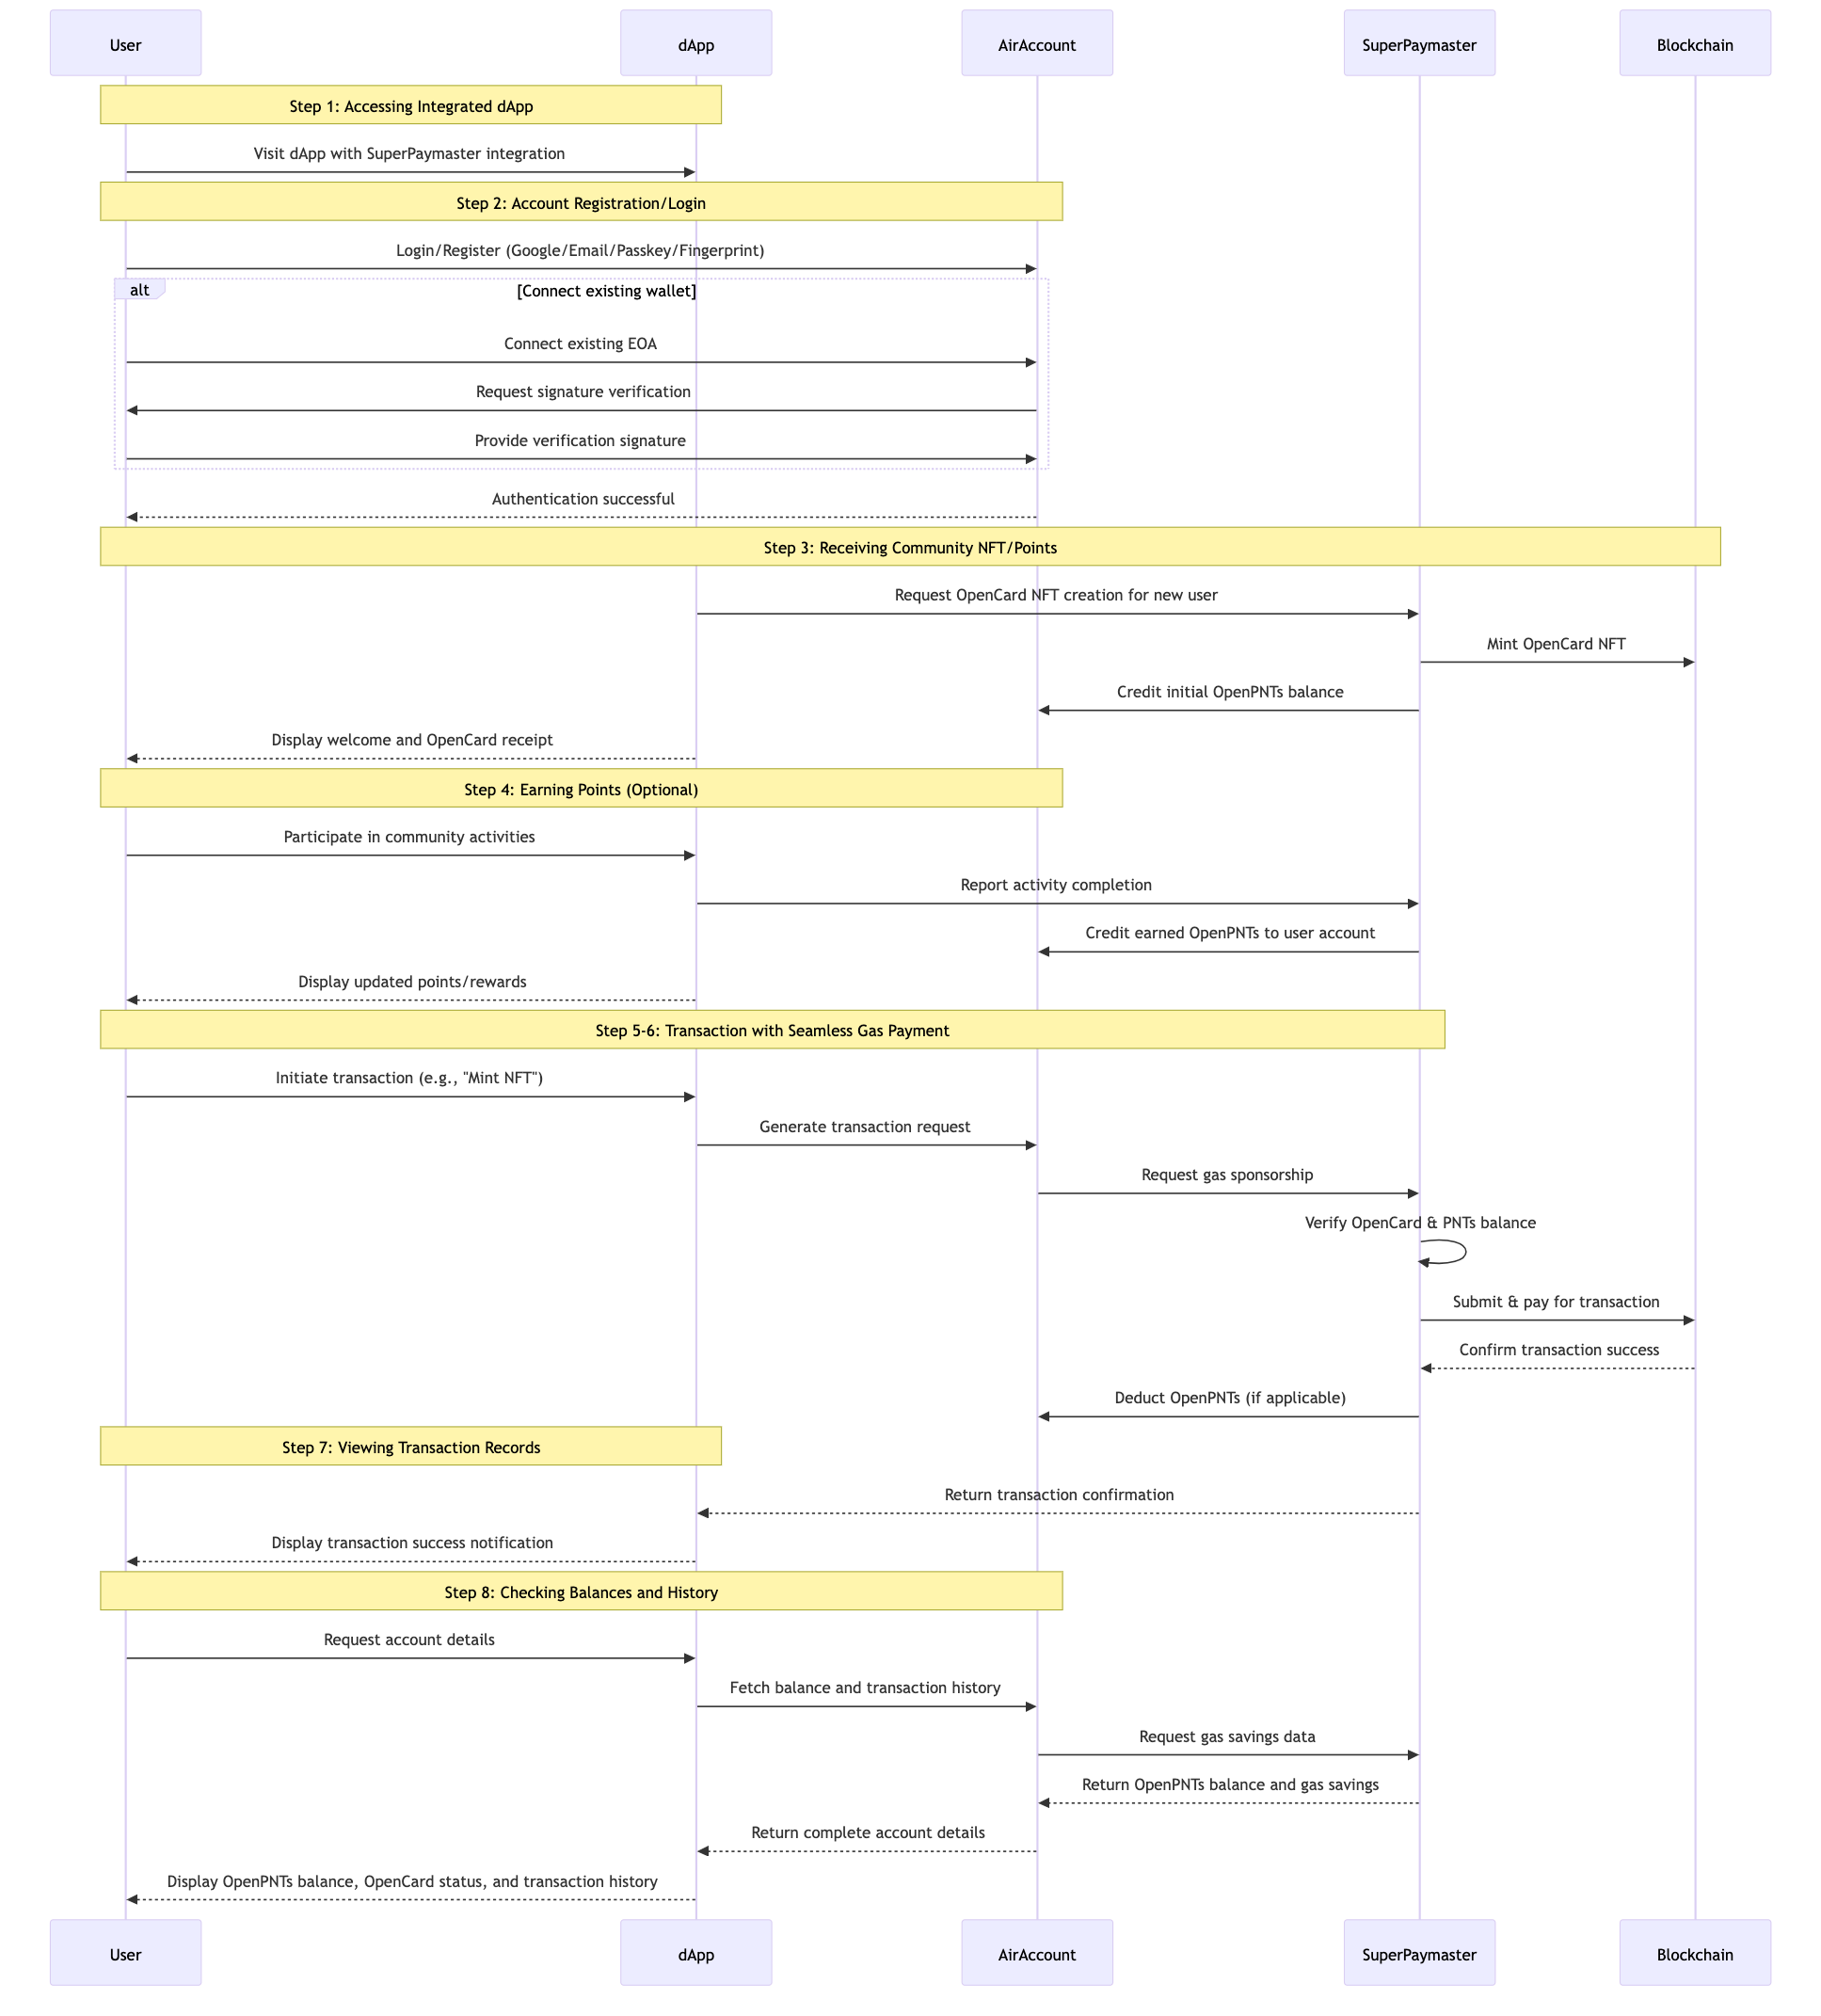
\includegraphics[width=0.9\textwidth]{user-interaction-workflow-figure}
\caption{User Interaction Workflow}
\label{fig:user-interaction-workflow}
\end{figure}

\section{Implementation (Proof of Concept - PoC)}
\label{sec:implementation}

This section details the Proof of Concept (PoC) implementation of the SuperPaymaster platform, covering smart contract development, the Standardized Decentralized Service System (SDSS) backend, node management, and user interface construction. Technological choices focused on enabling core functionalities—decentralized gas sponsorship, competitive quoting, enhanced user experience, and meeting security and interoperability requirements.

The SuperPaymaster PoC utilized the following tools and frameworks: Smart Contracts: For unmutable consensus, we use Solidity\cite{solidity} within the Foundry\cite{foundry}, a high-performance contract development framework implemented the core SuperPaymaster contract and auxiliary contracts for ENS resolution, OpenPNTs (ERC-20), OpenCards (ERC-721), and node registration which based on open source infrastructure. User Interfaces: Use popular and easy-to-use JavaScript/TypeScript framework, Next.js\cite{nextjs} (React\cite{react}, Node.js\cite{nodejs}) built web frontends. Desktop Clients: Tauri\cite{tauri} packaged cross-platform clients (Windows, MacOS, Linux, iOS, Android, Web) supporting N0 user nodes and N1 service nodes. Backend Services: High concurrency support, Go Golang\cite{golang} and Rust\cite{rust} developed backend/node on libp2p; Rust targeted performance-critical components and potential TEE-based services (N2 nodes). Deployment \& Infrastructure: Docker\cite{docker} provided containerization. A customized Supabase\cite{supabase} instance handled BaaS, database, and storage functionalities (N3 nodes). Account Management: The permissionless AirAccount API\cite{airaccount} managed user account lifecycles, security, and authentication. Hardware Testing on Decentralized Physical Infrastructure Networks(DePIN)\cite{depin2023}. We use high performance and Affordable for everyone like NXP i MX95(or TI AM64xx) served as representative compute nodes in production, use Raspberry Pi 5B 16G for developing and testing\cite{nxp-imx95}.

\subsection{System Setup and Configuration}
\label{subsec:system-setup}

We need to setup AirAccount, SuperPaymaster Nodes Configuration, to set interaction config with decentralized account supporting gas sponsorship, and a basic config for OpenPNTs, OpenCards and more parameters to pay your gas seemlessly. Also we need create cross-chain CometENS API name for node registry to get decentralized invoking. Anyone can run a node to act as a Paymaster Service Provider with their Secp256k1 key staked and registered on-chain with their own ERC20 gas token.

\begin{verbatim}
{
    "name": "AAstar SuperPaymaster Config Demo",
    "description": "A decentralized gas sponsor provider node",
    "image": "https://aastar.io/superpaymaster.png",
    "url": "https://aastar.io/superpaymaster",
    "ens": "paymaster.aastar.eth",
    "address": "0x1234567890123456789012345678901234567890",
    "stake": {
        "eth": "1000",
        "aastar": "1000",
        "promise": {
            "duration": "30d",
            "amount": "1000",
            "item": "url/ipfs",
            "token-accept": {
                "eth": "0x0000000000000000000000000000000000000000",
                "astPNTs": "0x1234567890123456789012345678901234567890",
                "USDT": "0x1234567890123456789012345678901234567890",
                "USDC": "0x1234567890123456789012345678901234567890",
                "DAI": "0x1234567890123456789012345678901234567890",
                "WETH": "0x1234567890123456789012345678901234567890"
            },
            "price": {
                "eth": "30",
                "astPNTs": "30",
                "USDT": "30",
                "USDC": "30",
                "DAI": "30",
                "WETH": "30"
            }
        }
    },
    "openpnts": {
        "factory": "0x1234567890123456789012345678901234567890",
        "PNTs": "0x1234567890123456789012345678901234567890",
        "ratio": "ratio.aastar.eth",
        "symbol": "astPNTs"
    },
    "opencards": {
        "factory": "0x1234567890123456789012345678901234567890",
        "nft": "0x1234567890123456789012345678901234567890",
        "ratio": "ratio.aastar.eth",
        "symbol": "astCards"
    },
    "Paymaster config": {
        "token-accept": [{
            "symbol": "astPNTs",
            "address": "0x1234567890123456789012345678901234567890",
            "price": "30"
        }, {
            "symbol": "xPNTs",
            "address": "0x0000000000000000000000000000000000000000",
            "price": "20"
        }],
        "limitation": {
            "daily": "1000",
            "single": "1 ETH"
        }
    }
}
\end{verbatim}

\subsection{Smart Contract Design and Development}
\label{subsec:smart-contract-design}

Smart contract is the key part of the system, through mutable on-chain code, to ensure verification of gas payment signatures, payment of gas, deduction of reasonable PNTs, allocation of PNTs income, calculation of reputation (success rate) and Slash etc. We only introduce core ability of SuperPaymaster contract, more details can be found in appendix.

1. Stake: Sub-account stake management for security and gas sponsor
2. Verify and Pay: Sub-account signature verification, payment, record and balance maintenance
3. Post Processing: Transaction success post processing: reputation increase
4. Compensation: Asynchronous transaction status compensation: failed and successful re-check, proof submission and reputation modification (off-chain, call on-chain method)

\subsubsection{SuperPaymaster Contract Flow}
\label{subsubsec:contract-flow}

\begin{figure}[htbp]
\centering
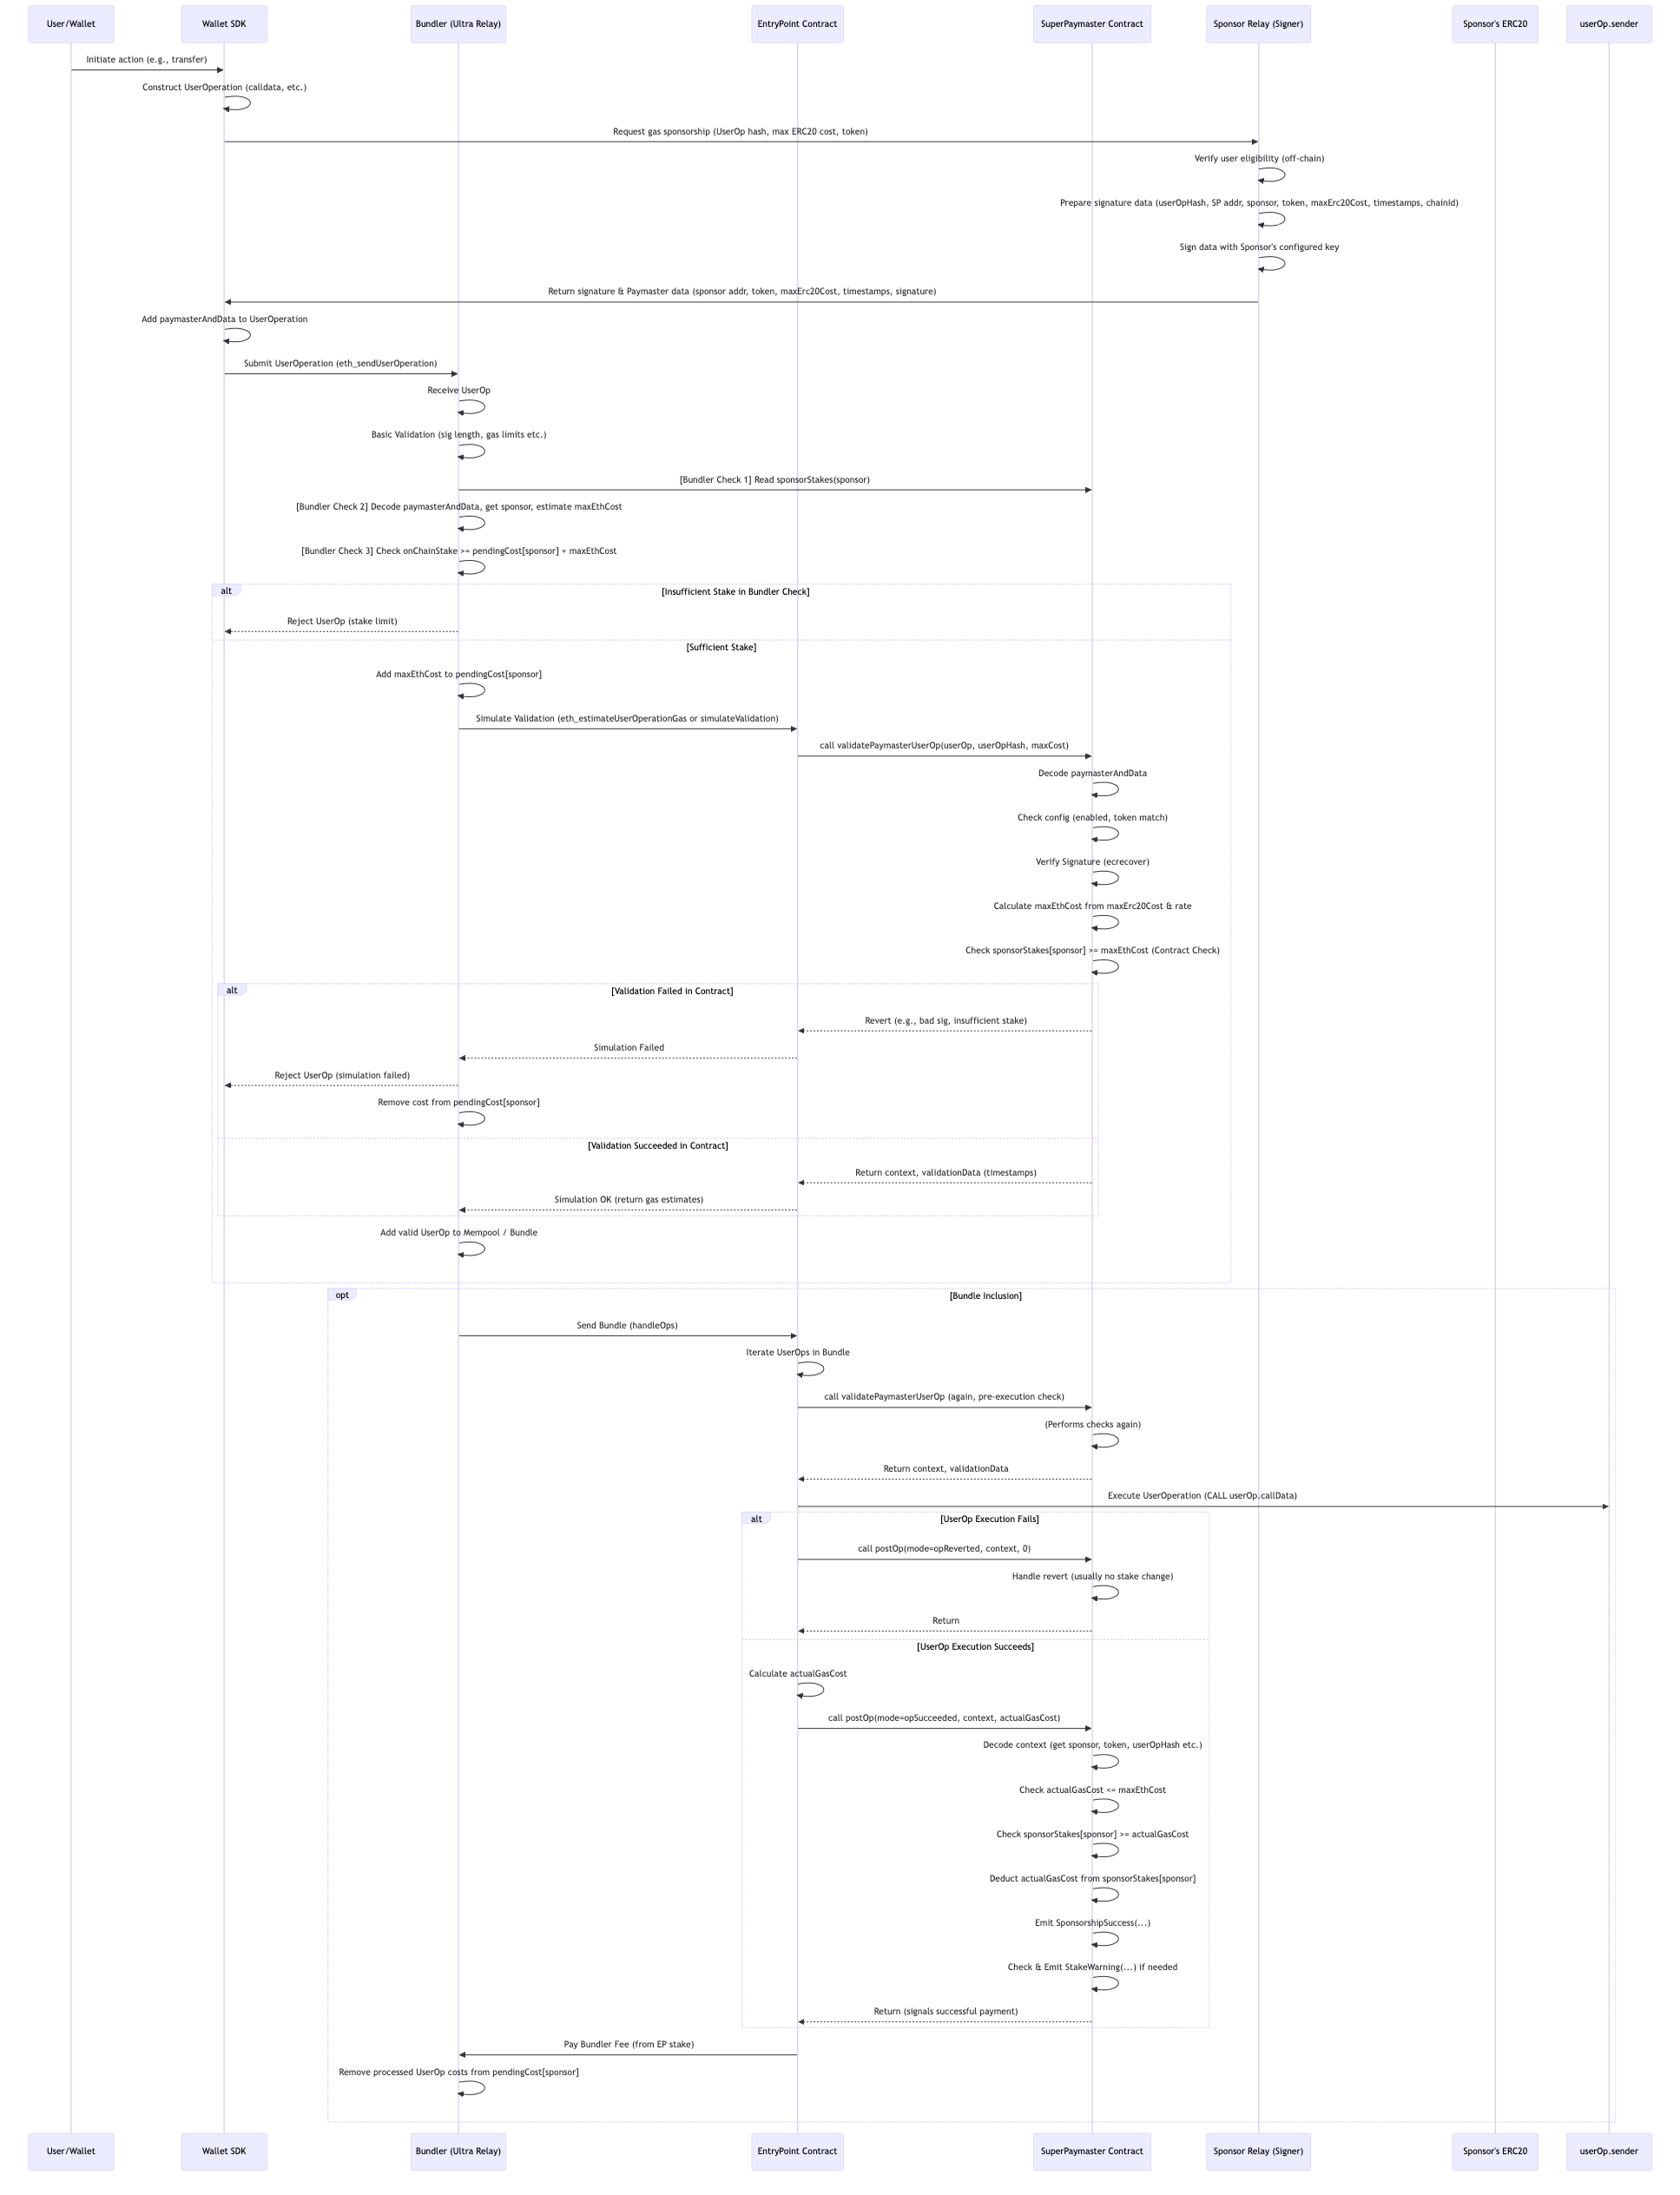
\includegraphics[width=0.9\textwidth]{superpaymaster-contract-flow-figure}
\caption{SuperPaymaster Contract Work Flow}
\label{fig:superpaymaster-contract-flow}
\end{figure}

\subsubsection{SuperPaymaster Contract Main Functions}
\label{subsubsec:contract-functions}

The smart contract has two main functions: stake and verifyAndPay, more details can be found in \cite{superpaymaster}. We build this contract based on ERC4337 and other Open-source projects: Pimilico singleton paymaster\cite{pimlico-singleton} and ZeroDev bundler\cite{zerodev-bundler}. We add sub-account stake module to permit permissionless staker to run their own paymaster for supporting their own ERC20 gas tokens. We improve verify function to avoid over-use risk with on-chain contract and off-chain bundler. Also we build SuperPaymaster relay server framework to support dApps to query gas price and pay gas with different ERC20 supporting. Stake manager contract provide a stake reputation and ETH payment guarantee for every ERC20 gas payment.

\begin{verbatim}
// SuperPaymaster.sol main function1: Stake manager

    /*                                                              */
    /*                    SPONSOR MANAGEMENT                       */
    /*                                                              */

    /**
     * @notice Set the withdrawal delay period
     * @param _withdrawalDelay New delay period in seconds
     */
    function setWithdrawalDelay(uint256 _withdrawalDelay) external onlyAdminOrManager {
        require(_withdrawalDelay > 0, "SuperPaymaster: withdrawal delay must be positive");
        withdrawalDelay = _withdrawalDelay;
    }

    /**
     * @inheritdoc ISuperPaymaster
     */
    function registerSponsor(address sponsor) external override onlyAdminOrManager {
        require(!isSponsor[sponsor], "SuperPaymaster: sponsor already registered");
        isSponsor[sponsor] = true;
        
        // Initialize with default config (owner = sponsor itself)
        sponsorConfigs[sponsor] = SponsorConfig({
            owner: sponsor,
            token: address(0),
            exchangeRate: 0,
            warningThreshold: 0,
            isEnabled: false,
            signer: address(0)
        });
        
        emit SponsorRegistered(sponsor);
    }

    /**
     * @inheritdoc ISuperPaymaster
     */
    function setSponsorConfig(
        address token,
        uint256 exchangeRate,
        uint256 warningThreshold,
        address signer
    ) external override {
        address sponsor = msg.sender;
        require(isSponsor[sponsor], "SuperPaymaster: not a sponsor");
        require(msg.sender == sponsorConfigs[sponsor].owner, "SuperPaymaster: only sponsor can modify settings");
        require(token != address(0), "SuperPaymaster: invalid token address");
        require(signer != address(0), "SuperPaymaster: invalid signer address");
        
        SponsorConfig storage config = sponsorConfigs[sponsor];
        config.token = token;
        config.exchangeRate = exchangeRate;
        config.warningThreshold = warningThreshold;
        config.signer = signer;
        
        emit SponsorConfigSet(sponsor, token, exchangeRate, warningThreshold, signer);
    }
\end{verbatim}

verifyAndPay provides a security guarantee for dApps to pay gas with different ERC20 tokens under their credit stake amount.

\begin{verbatim}
// SuperPaymaster.sol main function2: verifyAndPay
    function validateSponsorUserOp(
        PackedUserOperation calldata userOp,
        bytes32 userOpHash,
        uint256 /*requiredPreFund*/,
        bool allowAllBundlers,
        bytes calldata paymasterConfig
    ) internal returns (bytes memory context, uint256 validationData) {
        // check bundler authorization
        if (!allowAllBundlers && !isBundlerAllowed[tx.origin]) {
            revert BundlerNotAllowed(tx.origin);
        }
    
        // check replay attack
        require(!processedOps[userOpHash], "SuperPaymaster: operation hash already processed");
    
        // parse sponsor data
        (
            address sponsor,
            address token,
            uint256 maxErc20Cost,
            uint48 validUntil,
            uint48 validAfter,
            bytes calldata signature
        ) = _parseSponsorConfig(paymasterConfig);
        
        // verify sponsor is valid
        require(isSponsor[sponsor], "SuperPaymaster: invalid sponsor");
        require(sponsorConfigs[sponsor].isEnabled, "SuperPaymaster: sponsor not enabled");
        
        // verify token is matched
        require(token == sponsorConfigs[sponsor].token, "SuperPaymaster: token mismatch");
        
        // get sponsor signer
        address signer = sponsorConfigs[sponsor].signer;
        
        // create message hash for signature verification
        bytes32 hash = _getSponsorHash(userOp, userOpHash, sponsor, token, maxErc20Cost, validUntil, validAfter);
        
        // verify signature
        (bytes32 r, bytes32 s, uint8 v) = _extractSignature(signature);
        address recoveredSigner = ecrecover(hash, v, r, s);
        
        // check signature is valid
        if (recoveredSigner != signer) {
            revert("SuperPaymaster: invalid sponsor signature");
        }
        
        // calculate max ETH cost
        uint256 exchangeRate = sponsorConfigs[sponsor].exchangeRate;
        require(exchangeRate > 0, "SuperPaymaster: invalid exchange rate");
        
        // calculate maxEthCost: (maxErc20Cost * 1 ether) / exchangeRate
        uint256 maxEthCost = (maxErc20Cost * 1 ether) / exchangeRate;
        
        // get sponsor stake
        EnhancedSponsorStake storage stake = sponsorStakes[sponsor];
        
        // ensure sponsor has enough stake
        require(
            stake.stakedAmount >= maxEthCost,
            "SuperPaymaster: insufficient sponsor stake"
        );

        // lock this operation's funds
        if (stake.userOpLocks[userOpHash] == 0) {
            stake.lockedAmount += maxEthCost;
            stake.userOpLocks[userOpHash] = maxEthCost;
            emit StakeLocked(sponsor, userOpHash, maxEthCost);
        }
        
        // pack validation data (signature validity and timestamp)
        validationData = _packValidationData(false, validUntil, validAfter);
        
        // encode context for postOp
        context = abi.encode(sponsor, token, maxEthCost, maxErc20Cost, userOpHash);
        
        emit UserOperationSponsored(userOpHash, userOp.getSender(), SPONSOR_MODE, token, maxErc20Cost, maxEthCost);
        
        return (context, validationData);
    }
\end{verbatim}

\subsubsection{CometENS System Smart Contract}
\label{subsubsec:cometens-contract}

ENS is integral to SDSS, providing decentralized registration and discovery for services. Our CometENS solution utilizes ENS to allow stakers to register unique cross-chain service identifiers and store structured on-chain data (JSON via Text records). This supports dynamic discovery and configuration. Crucially, ENS also improves usability by mapping addresses to human-readable names—analogous to OpenCards' payment metaphor—leveraging users' understanding of domain systems to simplify interaction with blockchain identifiers.

A typical JSON config in ENS text record:

\begin{verbatim}
baseURL = "https://api.aastar.io";
baseENS = "api.aastar.eth";
nodeName = "XXXDAO";
serviceList = [{
    name: "getAPIList",
    description: "return API list",
    method: "GET",
    path: "/api/v1/getAPIList",
    params: [],
    response: [{
        name: "name",
        type: "string",
        required: true,
    }],
}, {
    name: "getAcceptERC20List",
    description: "return Accept ERC20 list",
    method: "GET",
    path: "/api/v1/getAcceptERC20List",
    params: [],
    response: [{
        symbol: "astPNTs",
        address: "0x0000000000000000000000000000000000000000",
        price: "30",
    }],
}, {
    name: "getSignature",
    description: "return Tx signature",
    method: "POST",
    path: "/api/v1/getSignature",
    params: [{
        name: "tx data",
        type: "json",
        required: true,
    }],
    response: [{
        name: "tx data signature",
        type: "string",
        required: true,
    }],
}];
\end{verbatim}

Besides setTextRecord, CometENS also provides normal wallet address setName and resolveName, setName to set your own node address, setAvatar to set your own wallet avatar, setContenthash to help node to have a readme web page in IPFS or other hash address.

\begin{figure}[htbp]
\centering
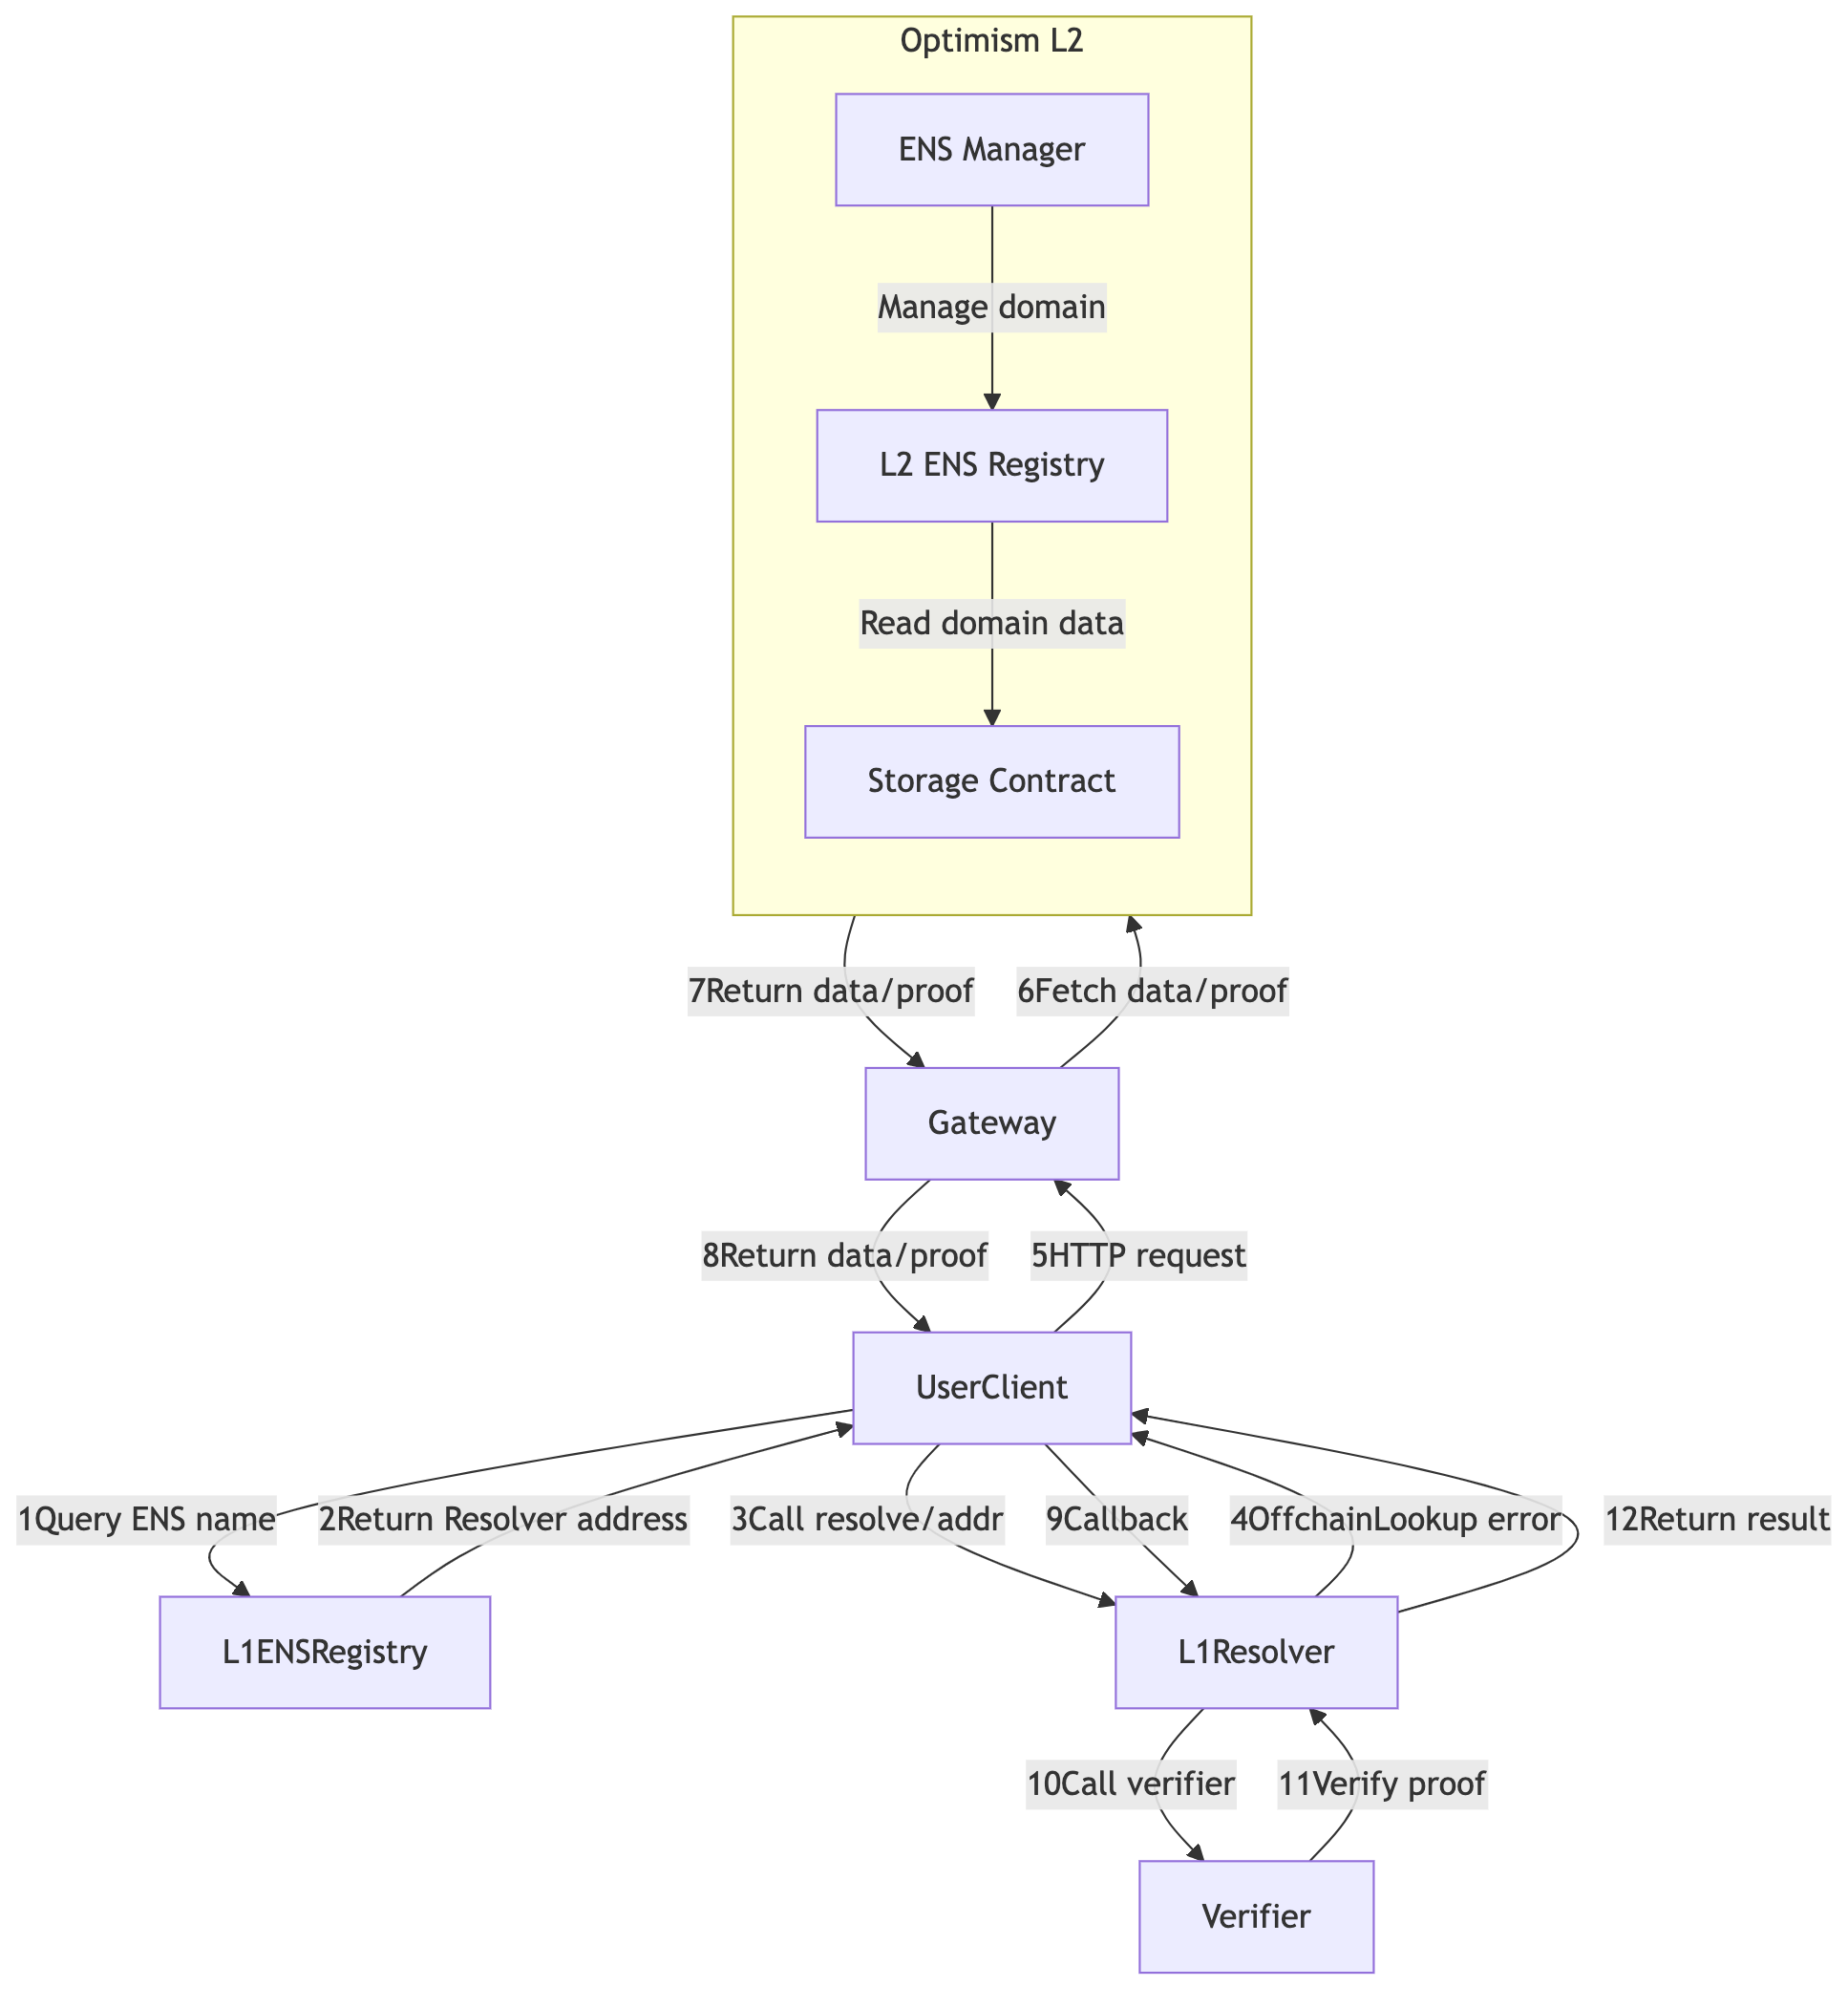
\includegraphics[width=0.8\textwidth]{node-registry-flow-figure2}
\caption{CometENS Flow}
\label{fig:cometens-flow}
\end{figure}

We need deploy a series of contracts in Optimism Layer2 and Ethereum mainnet.

\begin{figure}[htbp]
\centering
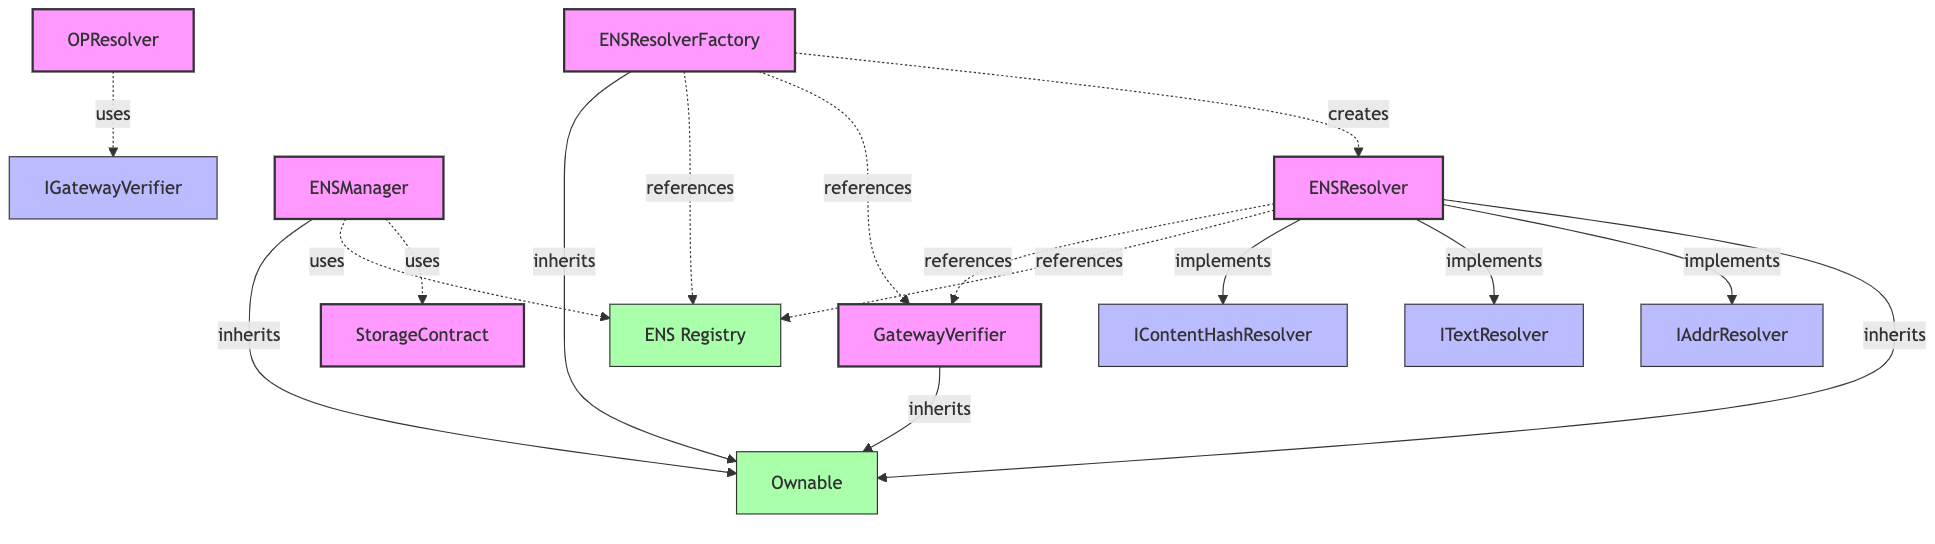
\includegraphics[width=0.8\textwidth]{backend-system-module-figure2}
\caption{Contracts Relation Graph}
\label{fig:contracts-relation}
\end{figure}

\subsubsection{OpenPNTs/OpenCards}
\label{subsubsec:openpnts-opencards}

We need a new token standard to support ERC20 gas token payment, named OpenPNTs. We also need a new NFT standard to support seamlessly gas payment, named OpenCards. The technical implementation of the OpenPNTs/OpenCards contract serves to realize the 'Gas Card and Points' metaphor, designed to abstract the complexities of gas payment for the end-user.

\subsection{AirAccount Integration}
\label{subsec:airaccount-integration}

SuperPaymaster need to integrate with AirAccount by API to support a totally user case flow for any transaction gas sponsor scenario. We assume any dApp(decentralized application) want to get a seamless and gasless transaction. We should provide the core APIs to support this flow:

1. after Next.js Application initiation.
2. install AirAccount SDK and SuperPaymaster SDK (both are in AAStar SDK)

\begin{verbatim}
pnpm install aastar/airaccount-sdk @aastar/superpaymaster-sdk
or 
pnpm install aastar
\end{verbatim}

3. Initiate an AirAccount account, used to save PNTs and test transactions.

\begin{verbatim}
aastar airaccount create //only support Email binding in command line
or use web page action
\end{verbatim}

4. Create a useroperation data(transaction data)

\begin{verbatim}
{  
  "sender": "0x...",          // User's account address (smart contract account)  
  "nonce": "0x...",           // Account's nonce for replay protection  
  "initCode": "0x...",        // Optional: Code to deploy the account if it doesn't exist  
  "callData": "0x...",        // The transaction payload to execute  
  "callGasLimit": "0x...",    // Gas limit for executing callData  
  "verificationGasLimit": "0x...", // Gas limit for account validation  
  "preVerificationGas": "0x...",  // Gas to cover off-chain costs (e.g., data gas)  
  "maxFeePerGas": "0x...",    // Maximum fee per gas for inclusion  
  "maxPriorityFeePerGas": "0x...", // Maximum priority fee per gas  
  "paymasterAndData": "0x...", // Paymaster address and data for gas sponsorship  
  "signature": "0x..."        // Signature authorizing the UserOperation  
}  
Gas payment information:
{
    paymentType: "ERC20/OpenCards/ETH" // ERC20 token and OpenCards credential
    // we support 3 types: ERC20 token(in your account balance), OpenCards(binding with a NFT card, use this balance) , and default ETH
    gasToken: "0x123..." // gas token address
    price: "30" // price per gas for gWei with one ERC20 token
}
\end{verbatim}

5. Follow the flow above, send to relay(provides bundler and paymaster service all in one)

\subsection{Backend Service Implementation}
\label{subsec:backend-implementation}

\subsubsection{Node Registry}

All backend services must first be registered as nodes. We use Next.js to interact with on-chain contract.

1. Generate a node public/private key pair.
2. Call the node registration contract (NodeRegistry) ABI to register the node.
3. Approving, staking and some form of authorization are required.
4. Then the node will can provide some decentralized services like paymaster sponsor services.
5. Follow the deployment documents to run a paymaster relay in your node.

\begin{figure}[htbp]
\centering
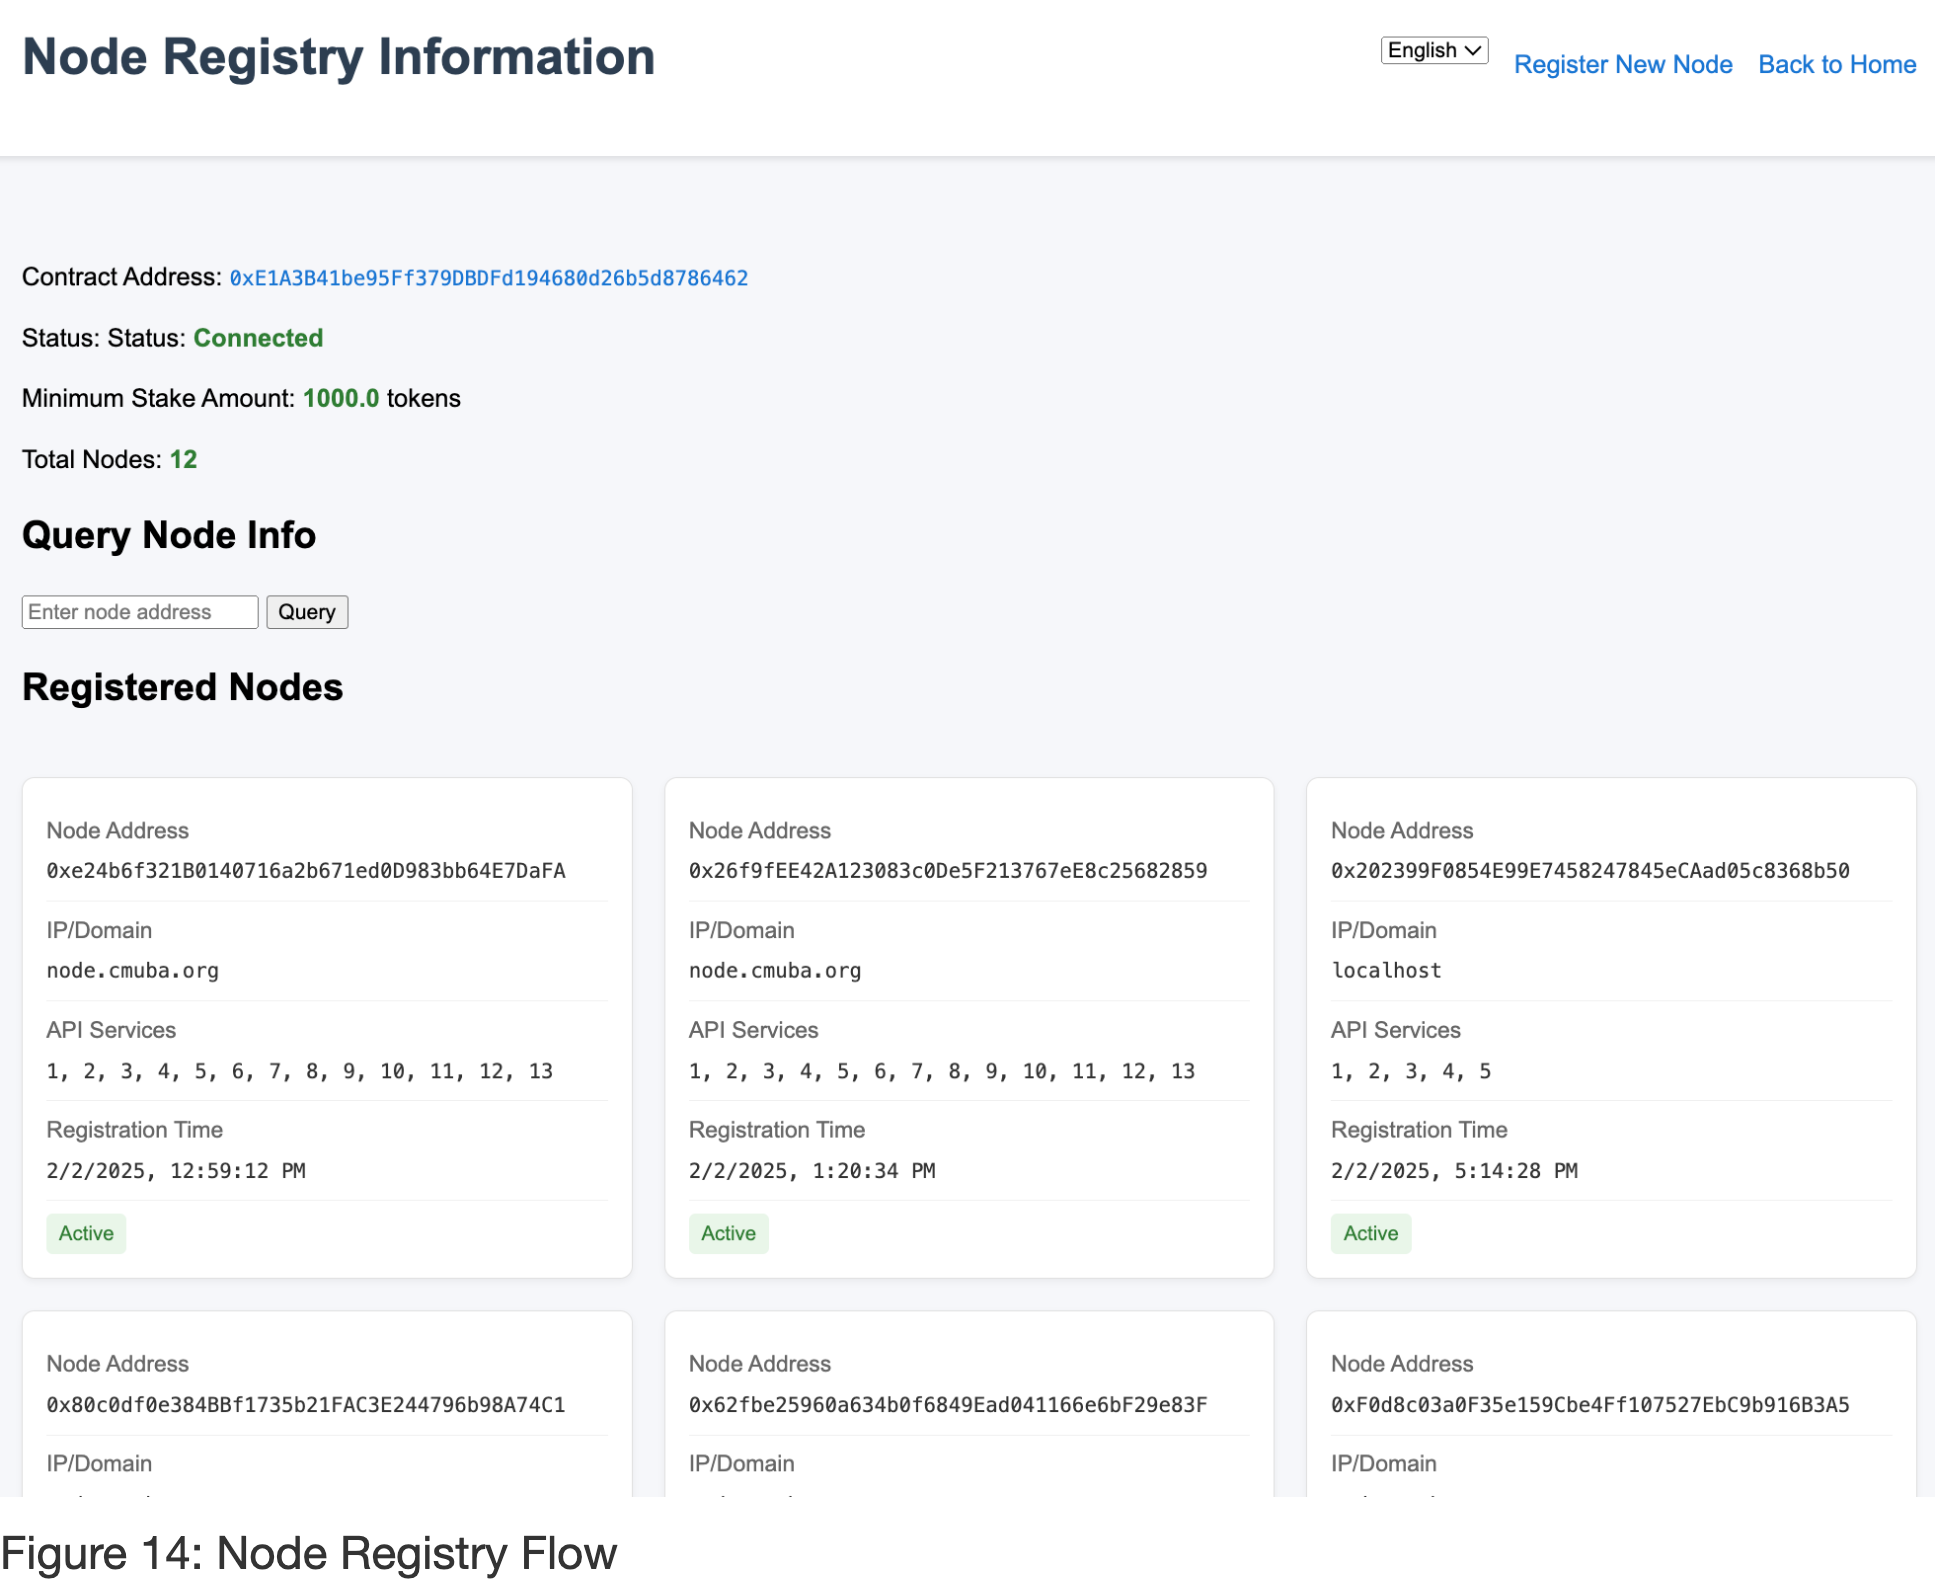
\includegraphics[width=0.8\textwidth]{node-registry-flow-figure}
\caption{Node Registry Flow}
\label{fig:node-registry-flow}
\end{figure}

\subsubsection{SuperPaymaster Relay Server}

We create a all-in-one relay server: provide paymaster signature and bundler service. So as the flow above mentioned, the dApp can create the useroperation and then send to the relay to launch the transaction in one time API invoking. We develope the relay based on ZeroDev's ultra relay \cite{zerodev-bundler} and Pimlico's Alto bundler \cite{pimlico-alto} source code.

Before a dApp invoking the relay server, you must use ethers.js or wagmi to get a random relay server API URI:

1. access website: paymaster.aastar.io(superpaymaster.aastar.io) or parse ENS: paymaster.aastar.eth(superpaymaster.aastar.eth) , get a paymaster collection like this:

\begin{verbatim}
{
    "paymasters": [
        {
            "address": "0x...",
            "name": "Paymaster 1",
            "ensName": "Paymaster1.0gas.aastar.eth",
            "description": "Description 1",
            "URL": "https://paymaster1.com/api",
            "price"{ //gwei price for token
                "eth": "30",
                "astPNTs": "30",
                "USDT": "30",
                "USDC": "30",
                "DAI": "30",
                "WETH": "30"
            }
        },
        {
            "address": "0x...",
            "name": "Paymaster 2",
            "ensName": "Paymaster2.0gas.aastar.eth",
            "description": "Description 2",
            "URL": "https://paymaster2.com/api",
            "price": {
                "eth": "30",
                "astPNTs": "30",
                "USDT": "30",
                "USDC": "30",
                "DAI": "30",
                "WETH": "30"
            }
        }
    ]
}
\end{verbatim}

The website will refresh every 10 minutes from on-chain text record. The ENS name is realtime(depneds on the specific layer2 sync cycle with layer1). The URL is the API endpoint for the paymaster service. You can remember the paymaster1.0gas.aastar.eth and paymaster2.0gas.aastar.eth to get refresh changes. 

2. Determine the fittable paymaster you want to use based on your token type and affordable price, get the URL to invoke. 
3. Send the useroperation to the relay server. 
4. The relay server will return the paymaster signature and original transaction data.

Let's know the basic flow:

1. whoRU: SuperPaymaster relay server will returen the node identity: address, ENS name, public key and ERC20 gas token support list with price.
2. \_isRegistered: SuperPaymaster contract can verify whether the node is registered and get the stake amount and reputation.
3. getSignature: SuperPaymaster relay server receive dApps useroperation and gas payment config, then return the paymaster signature and original transaction data.
4. \_verifySecondSignature: It is a validator module of relay server to operate the dApps request, validate transaction data and user's finger-print signature.
5. \_signPaymasterAndData: SuperPaymaster relay server sign siganature after verification.
6. \_signTEE, it is a extend function of validator with a ARM chips.
7. \_payERC20Gas: SuperPaymaster will check the OpenCard NFT ERC20 balance or account PNTs balance and deduct PNTs firstly.
8. \_postPayment: if sponsor successsfully, refund PNTs and calculate the node reputation.
9. \_simulateTx: try to simulate the transaction data verify and submit, if passed, send to RPC. It is a bunlder module.

\subsection{SDSS(Standard Decentralized Service System) Implementation Details}
\label{subsec:sdss-implementation}

Every application require a backend service or cloud computing service. We create SDSS as a decentralized computing service system that provides a rain computing service for decentralized applications. We have design and evaluate the SDSS system, for the initial version, we will provide a simple service package.

1. A Tauri based cross platform client SDK, anyone can develop their own dApp with this framework with Rust.
2. A permissionless node registry to stake and run your own rain computing node, include CometENS and node management contract with Node.js.
3. A recommandation hardware for developing mode: Raspberry 5B based TEE+hardware wallet node, include hardware wallet and TEE security module in Rust.
4. A open source infura service package:
   1. Bundler: Ultra Relay +(contract and SDK in Node.js)
   2. Paymaster: SuperPaymaster (contract, relay and SDK in Node.js and Go)
   3. Account: AirAccount (contract and SDK in Node.js, Rust and Go)
   4. Validator: BLS+TEE(service and SDK in Node.js)
   5. BaaS: Supabase(SDK in Go and Node.js)
   6. User dApps Demo: COS72 (SDK and demo in Node.js and Rust)
   7. Node management: COS72 Community Panel(UI application) in Node.js and Rust.
   8. Docker image: AAStar All regions are categorized by CPU type into ARM, x86, and others. Each region is divided into two parts: User and Community. These two parts have overlapping areas where users with spare computing power act as community computing nodes. User section: Tauri cross-platform client, providing an interactive interface for dApps, can run on any device. Community section: For non-ARM regions, users run Docker services including Bundler, Paymaster, Account, Validator, BaaS (Supabase), and other services. For ARM regions, added TEE hardware wallet + signature service + privacy computing service. Community section: A community panel provides a management portal for configuring all backend services. Hardware DePIN recommendation: Raspberry Pi 5B 16G(for developement), running Docker + TEE is sufficient to serve a small community. 

We have a backend system module structure graph:

\subsubsection{CometENS System Smart Contract}
\label{subsubsec:cometens-contract}

ENS is integral to SDSS, providing decentralized registration and discovery for services. Our CometENS solution utilizes ENS to allow stakers to register unique cross-chain service identifiers and store structured on-chain data (JSON via Text records). This supports dynamic discovery and configuration. Crucially, ENS also improves usability by mapping addresses to human-readable names—analogous to OpenCards' payment metaphor—leveraging users' understanding of domain systems to simplify interaction with blockchain identifiers.

A typical JSON config in ENS text record:

\begin{verbatim}
baseURL = "https://api.aastar.io";
baseENS = "api.aastar.eth";
nodeName = "XXXDAO";
serviceList = [{
    name: "getAPIList",
    description: "return API list",
    method: "GET",
    path: "/api/v1/getAPIList",
    params: [],
    response: [{
        name: "name",
        type: "string",
        required: true,
    }],
}, {
    name: "getAcceptERC20List",
    description: "return Accept ERC20 list",
    method: "GET",
    path: "/api/v1/getAcceptERC20List",
    params: [],
    response: [{
        symbol: "astPNTs",
        address: "0x0000000000000000000000000000000000000000",
        price: "30",
    }],
}, {
    name: "getSignature",
    description: "return Tx signature",
    method: "POST",
    path: "/api/v1/getSignature",
    params: [{
        name: "tx data",
        type: "json",
        required: true,
    }],
    response: [{
        name: "tx data signature",
        type: "string",
        required: true,
    }],
}];
\end{verbatim}

Besides setTextRecord, CometENS also provides normal wallet address setName and resolveName, setName to set your own node address, setAvatar to set your own wallet avatar, setContenthash to help node to have a readme web page in IPFS or other hash address.

\begin{figure}[htbp]
\centering
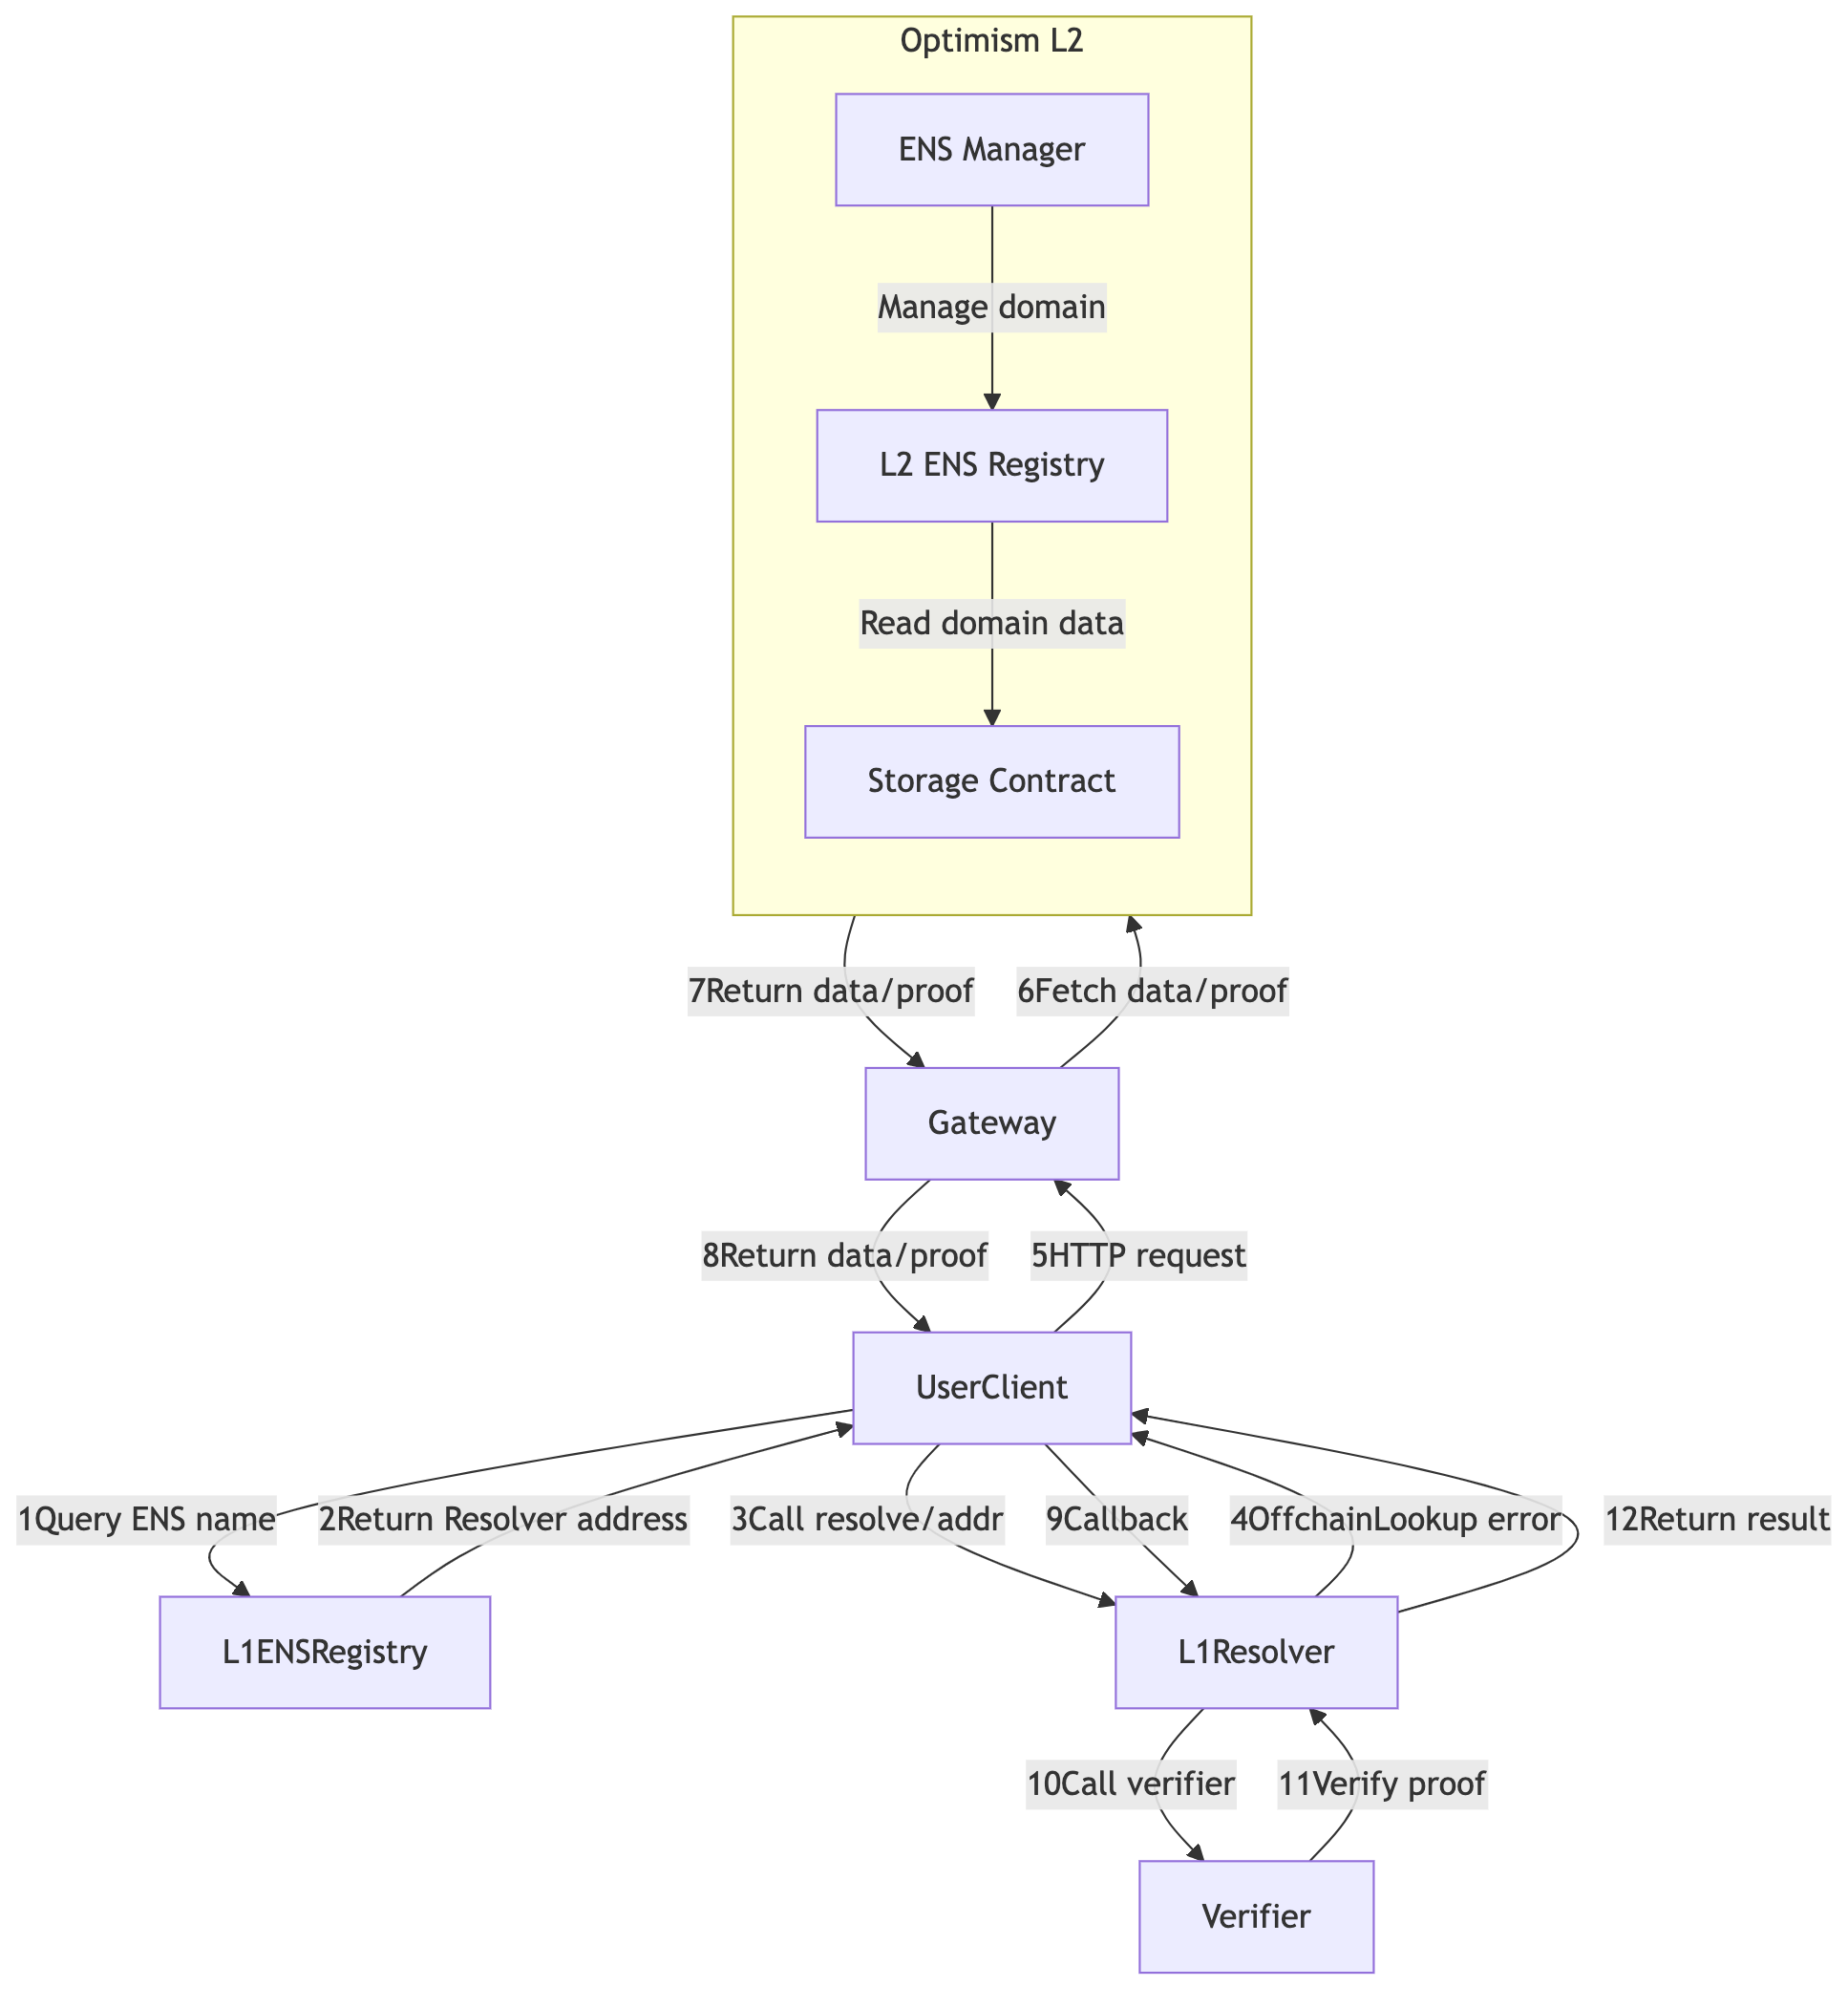
\includegraphics[width=0.8\textwidth]{node-registry-flow-figure2}
\caption{CometENS Flow}
\label{fig:cometens-flow}
\end{figure}

We need deploy a series of contracts in Optimism Layer2 and Ethereum mainnet.

\begin{figure}[htbp]
\centering
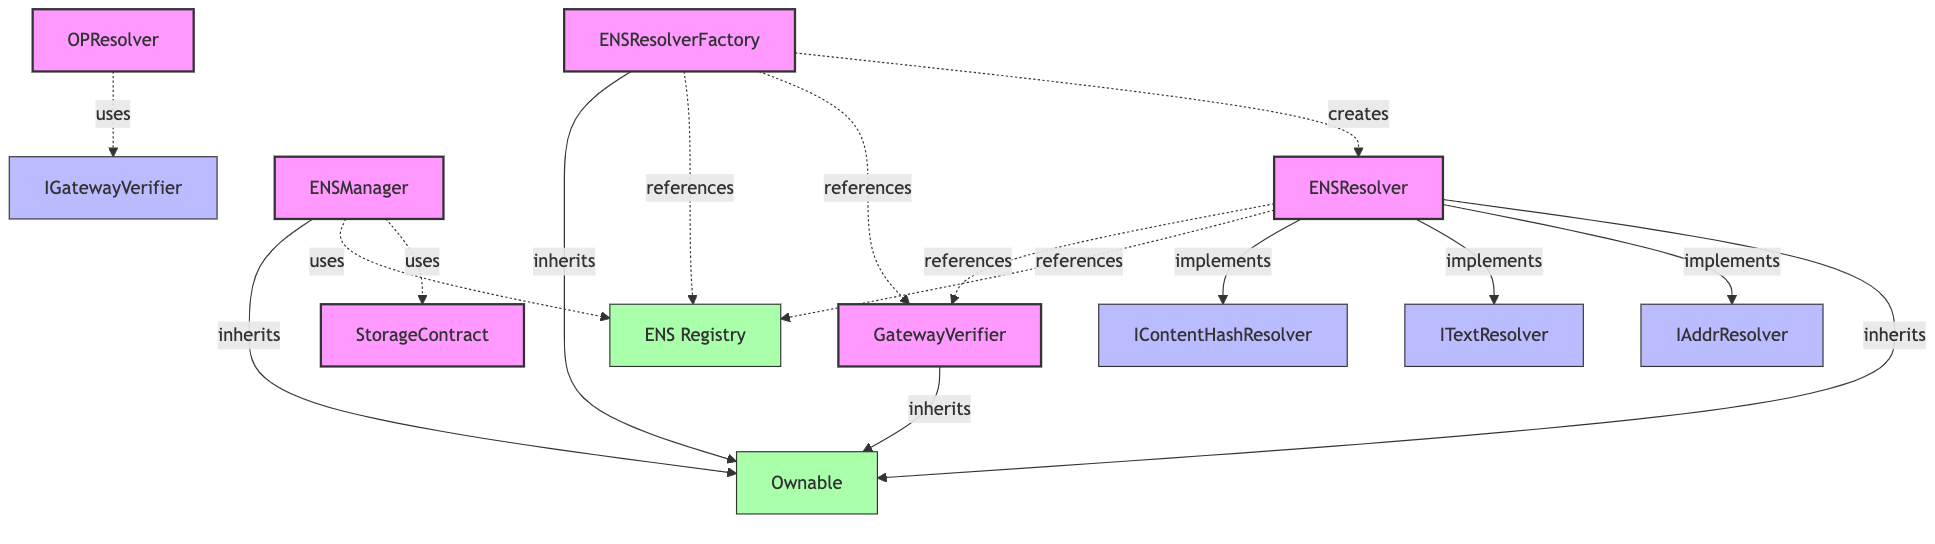
\includegraphics[width=0.8\textwidth]{backend-system-module-figure2}
\caption{Contracts Relation Graph}
\label{fig:contracts-relation}
\end{figure}

\subsubsection{OpenPNTs/OpenCards}
\label{subsubsec:openpnts-opencards}

We need a new token standard to support ERC20 gas token payment, named OpenPNTs. We also need a new NFT standard to support seamlessly gas payment, named OpenCards. The technical implementation of the OpenPNTs/OpenCards contract serves to realize the 'Gas Card and Points' metaphor, designed to abstract the complexities of gas payment for the end-user.

\subsection{AirAccount Integration}
\label{subsec:airaccount-integration}

SuperPaymaster need to integrate with AirAccount by API to support a totally user case flow for any transaction gas sponsor scenario. We assume any dApp(decentralized application) want to get a seamless and gasless transaction. We should provide the core APIs to support this flow:

1. after Next.js Application initiation.
2. install AirAccount SDK and SuperPaymaster SDK (both are in AAStar SDK)

\begin{verbatim}
pnpm install aastar/airaccount-sdk @aastar/superpaymaster-sdk
or 
pnpm install aastar
\end{verbatim}

3. Initiate an AirAccount account, used to save PNTs and test transactions.

\begin{verbatim}
aastar airaccount create //only support Email binding in command line
or use web page action
\end{verbatim}

4. Create a useroperation data(transaction data)

\begin{verbatim}
{  
  "sender": "0x...",          // User's account address (smart contract account)  
  "nonce": "0x...",           // Account's nonce for replay protection  
  "initCode": "0x...",        // Optional: Code to deploy the account if it doesn't exist  
  "callData": "0x...",        // The transaction payload to execute  
  "callGasLimit": "0x...",    // Gas limit for executing callData  
  "verificationGasLimit": "0x...", // Gas limit for account validation  
  "preVerificationGas": "0x...",  // Gas to cover off-chain costs (e.g., data gas)  
  "maxFeePerGas": "0x...",    // Maximum fee per gas for inclusion  
  "maxPriorityFeePerGas": "0x...", // Maximum priority fee per gas  
  "paymasterAndData": "0x...", // Paymaster address and data for gas sponsorship  
  "signature": "0x..."        // Signature authorizing the UserOperation  
}  
Gas payment information:
{
    paymentType: "ERC20/OpenCards/ETH" // ERC20 token and OpenCards credential
    // we support 3 types: ERC20 token(in your account balance), OpenCards(binding with a NFT card, use this balance) , and default ETH
    gasToken: "0x123..." // gas token address
    price: "30" // price per gas for gWei with one ERC20 token
}
\end{verbatim}

5. Follow the flow above, send to relay(provides bundler and paymaster service all in one)

\subsection{Backend Service Implementation}
\label{subsec:backend-implementation}

\subsubsection{Node Registry}

All backend services must first be registered as nodes. We use Next.js to interact with on-chain contract.

1. Generate a node public/private key pair.
2. Call the node registration contract (NodeRegistry) ABI to register the node.
3. Approving, staking and some form of authorization are required.
4. Then the node will can provide some decentralized services like paymaster sponsor services.
5. Follow the deployment documents to run a paymaster relay in your node.

\begin{figure}[htbp]
\centering
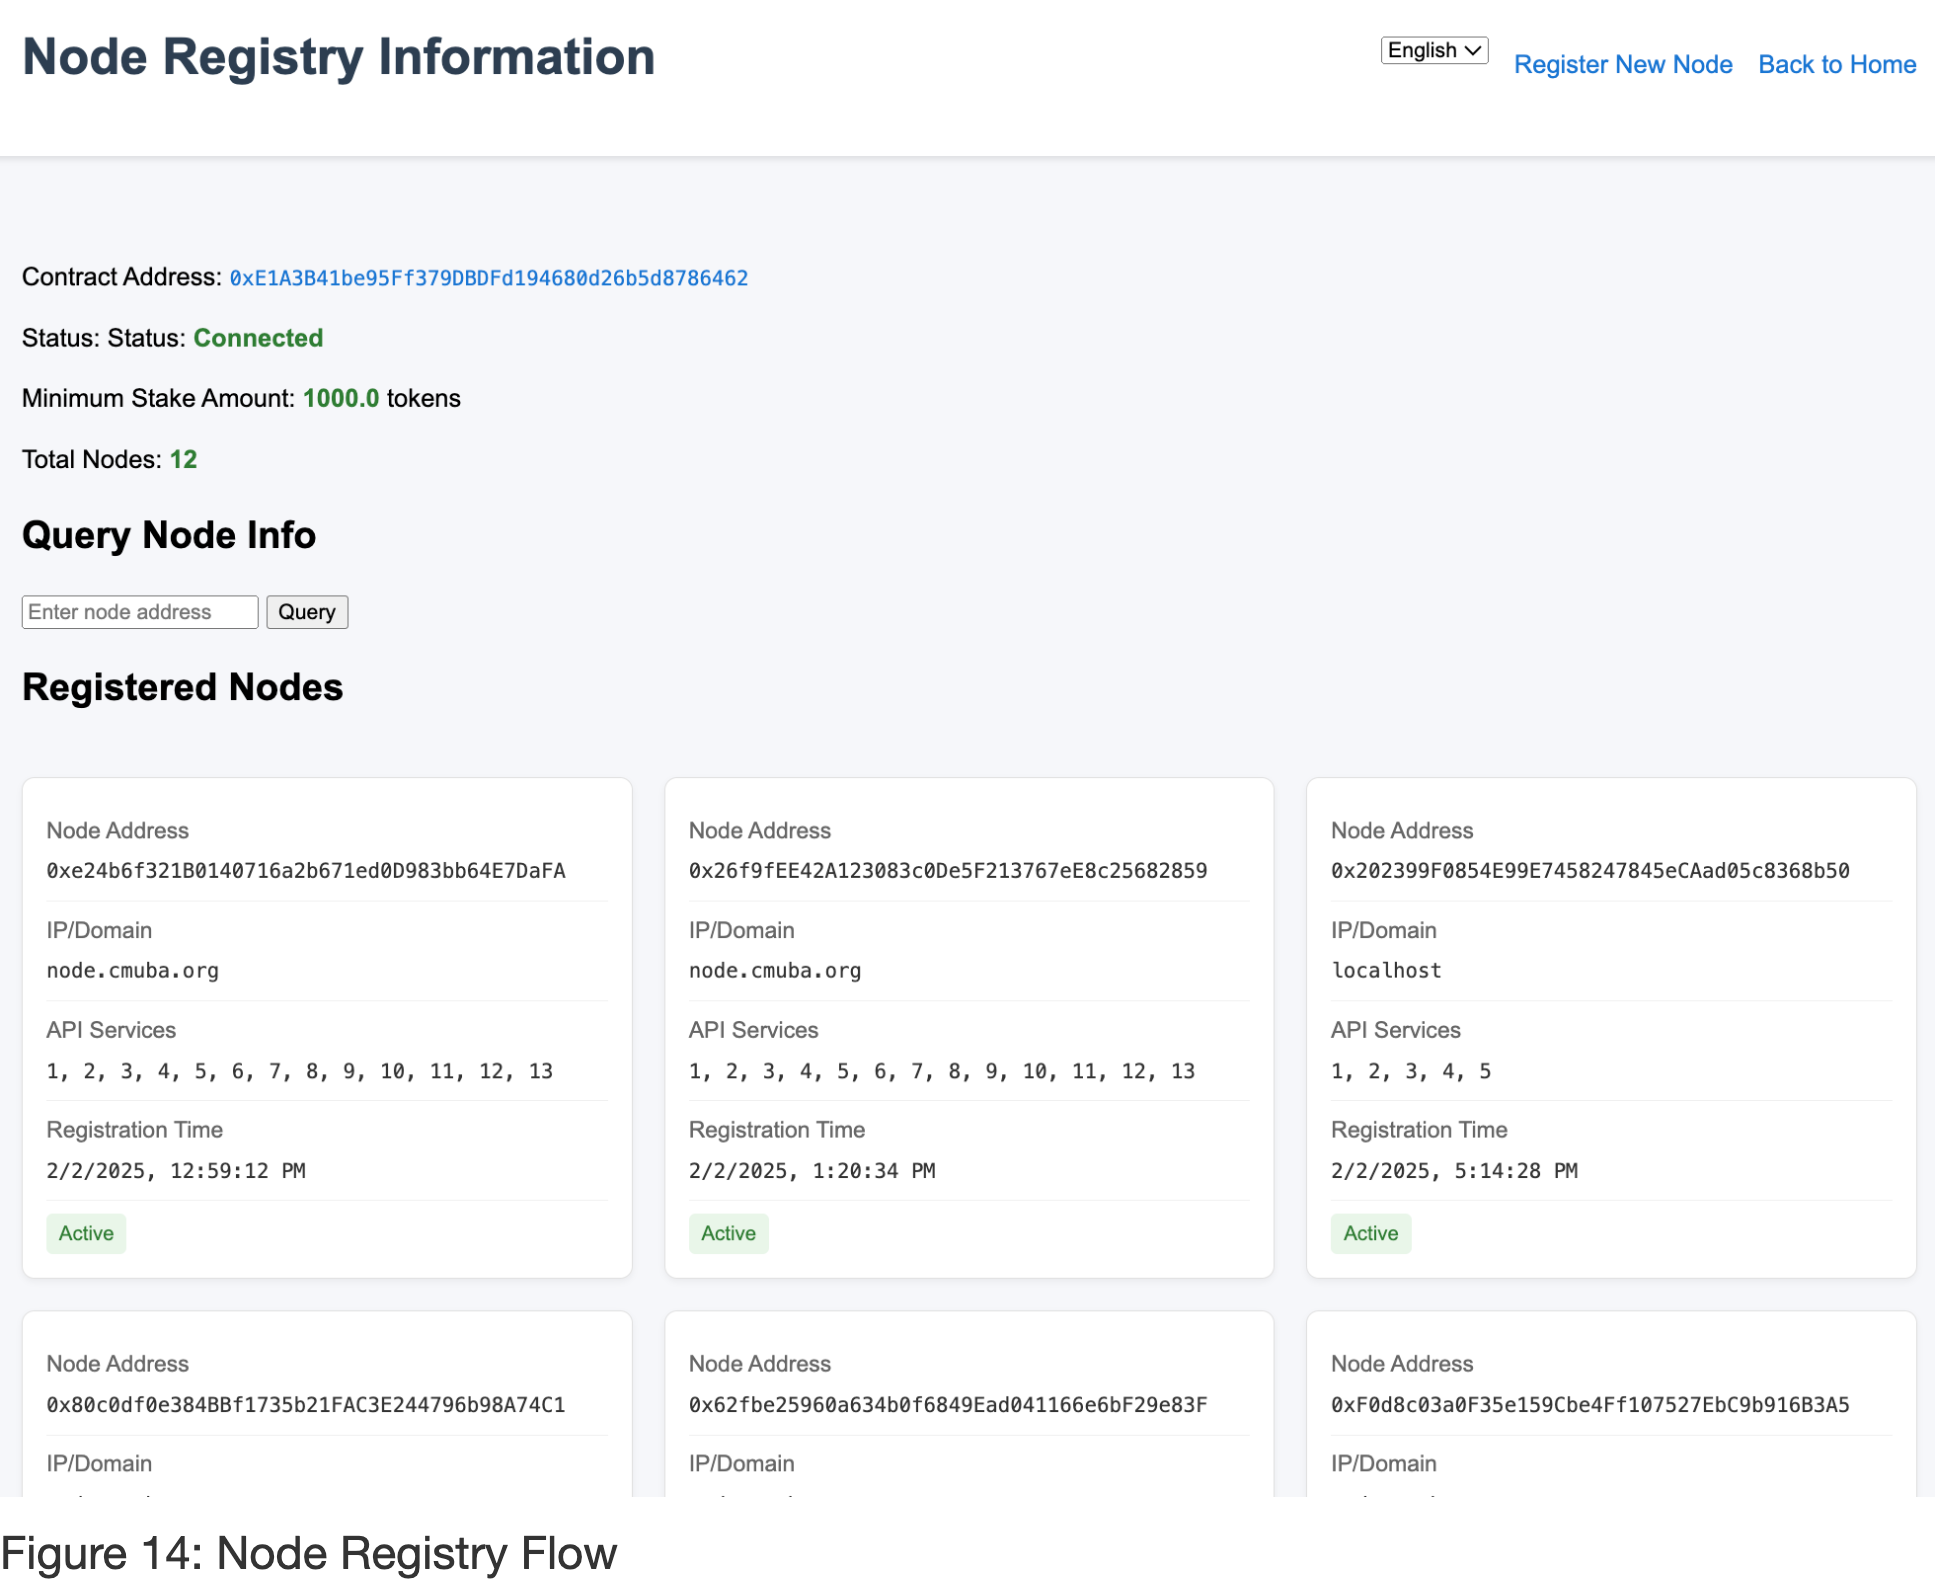
\includegraphics[width=0.8\textwidth]{node-registry-flow-figure}
\caption{Node Registry Flow}
\label{fig:node-registry-flow}
\end{figure}

\subsubsection{SuperPaymaster Relay Server}

We create a all-in-one relay server: provide paymaster signature and bundler service. So as the flow above mentioned, the dApp can create the useroperation and then send to the relay to launch the transaction in one time API invoking. We develope the relay based on ZeroDev's ultra relay \cite{zerodev-bundler} and Pimlico's Alto bundler \cite{pimlico-alto} source code.

Before a dApp invoking the relay server, you must use ethers.js or wagmi to get a random relay server API URI:

1. access website: paymaster.aastar.io(superpaymaster.aastar.io) or parse ENS: paymaster.aastar.eth(superpaymaster.aastar.eth) , get a paymaster collection like this:

\begin{verbatim}
{
    "paymasters": [
        {
            "address": "0x...",
            "name": "Paymaster 1",
            "ensName": "Paymaster1.0gas.aastar.eth",
            "description": "Description 1",
            "URL": "https://paymaster1.com/api",
            "price"{ //gwei price for token
                "eth": "30",
                "astPNTs": "30",
                "USDT": "30",
                "USDC": "30",
                "DAI": "30",
                "WETH": "30"
            }
        },
        {
            "address": "0x...",
            "name": "Paymaster 2",
            "ensName": "Paymaster2.0gas.aastar.eth",
            "description": "Description 2",
            "URL": "https://paymaster2.com/api",
            "price": {
                "eth": "30",
                "astPNTs": "30",
                "USDT": "30",
                "USDC": "30",
                "DAI": "30",
                "WETH": "30"
            }
        }
    ]
}
\end{verbatim}

The website will refresh every 10 minutes from on-chain text record. The ENS name is realtime(depneds on the specific layer2 sync cycle with layer1). The URL is the API endpoint for the paymaster service. You can remember the paymaster1.0gas.aastar.eth and paymaster2.0gas.aastar.eth to get refresh changes. 

2. Determine the fittable paymaster you want to use based on your token type and affordable price, get the URL to invoke. 
3. Send the useroperation to the relay server. 
4. The relay server will return the paymaster signature and original transaction data.

Let's know the basic flow:

1. whoRU: SuperPaymaster relay server will returen the node identity: address, ENS name, public key and ERC20 gas token support list with price.
2. \_isRegistered: SuperPaymaster contract can verify whether the node is registered and get the stake amount and reputation.
3. getSignature: SuperPaymaster relay server receive dApps useroperation and gas payment config, then return the paymaster signature and original transaction data.
4. \_verifySecondSignature: It is a validator module of relay server to operate the dApps request, validate transaction data and user's finger-print signature.
5. \_signPaymasterAndData: SuperPaymaster relay server sign siganature after verification.
6. \_signTEE, it is a extend function of validator with a ARM chips.
7. \_payERC20Gas: SuperPaymaster will check the OpenCard NFT ERC20 balance or account PNTs balance and deduct PNTs firstly.
8. \_postPayment: if sponsor successsfully, refund PNTs and calculate the node reputation.
9. \_simulateTx: try to simulate the transaction data verify and submit, if passed, send to RPC. It is a bunlder module.

\subsection{SDSS(Standard Decentralized Service System) Implementation Details}
\label{subsec:sdss-implementation}

Every application require a backend service or cloud computing service. We create SDSS as a decentralized computing service system that provides a rain computing service for decentralized applications. We have design and evaluate the SDSS system, for the initial version, we will provide a simple service package.

1. A Tauri based cross platform client SDK, anyone can develop their own dApp with this framework with Rust.
2. A permissionless node registry to stake and run your own rain computing node, include CometENS and node management contract with Node.js.
3. A recommandation hardware for developing mode: Raspberry 5B based TEE+hardware wallet node, include hardware wallet and TEE security module in Rust.
4. A open source infura service package:
   1. Bundler: Ultra Relay +(contract and SDK in Node.js)
   2. Paymaster: SuperPaymaster (contract, relay and SDK in Node.js and Go)
   3. Account: AirAccount (contract and SDK in Node.js, Rust and Go)
   4. Validator: BLS+TEE(service and SDK in Node.js)
   5. BaaS: Supabase(SDK in Go and Node.js)
   6. User dApps Demo: COS72 (SDK and demo in Node.js and Rust)
   7. Node management: COS72 Community Panel(UI application) in Node.js and Rust.
   8. Docker image: AAStar All regions are categorized by CPU type into ARM, x86, and others. Each region is divided into two parts: User and Community. These two parts have overlapping areas where users with spare computing power act as community computing nodes. User section: Tauri cross-platform client, providing an interactive interface for dApps, can run on any device. Community section: For non-ARM regions, users run Docker services including Bundler, Paymaster, Account, Validator, BaaS (Supabase), and other services. For ARM regions, added TEE hardware wallet + signature service + privacy computing service. Community section: A community panel provides a management portal for configuring all backend services. Hardware DePIN recommendation: Raspberry Pi 5B 16G(for developement), running Docker + TEE is sufficient to serve a small community. 

We have a backend system module structure graph:

\begin{figure}[htbp]
\centering
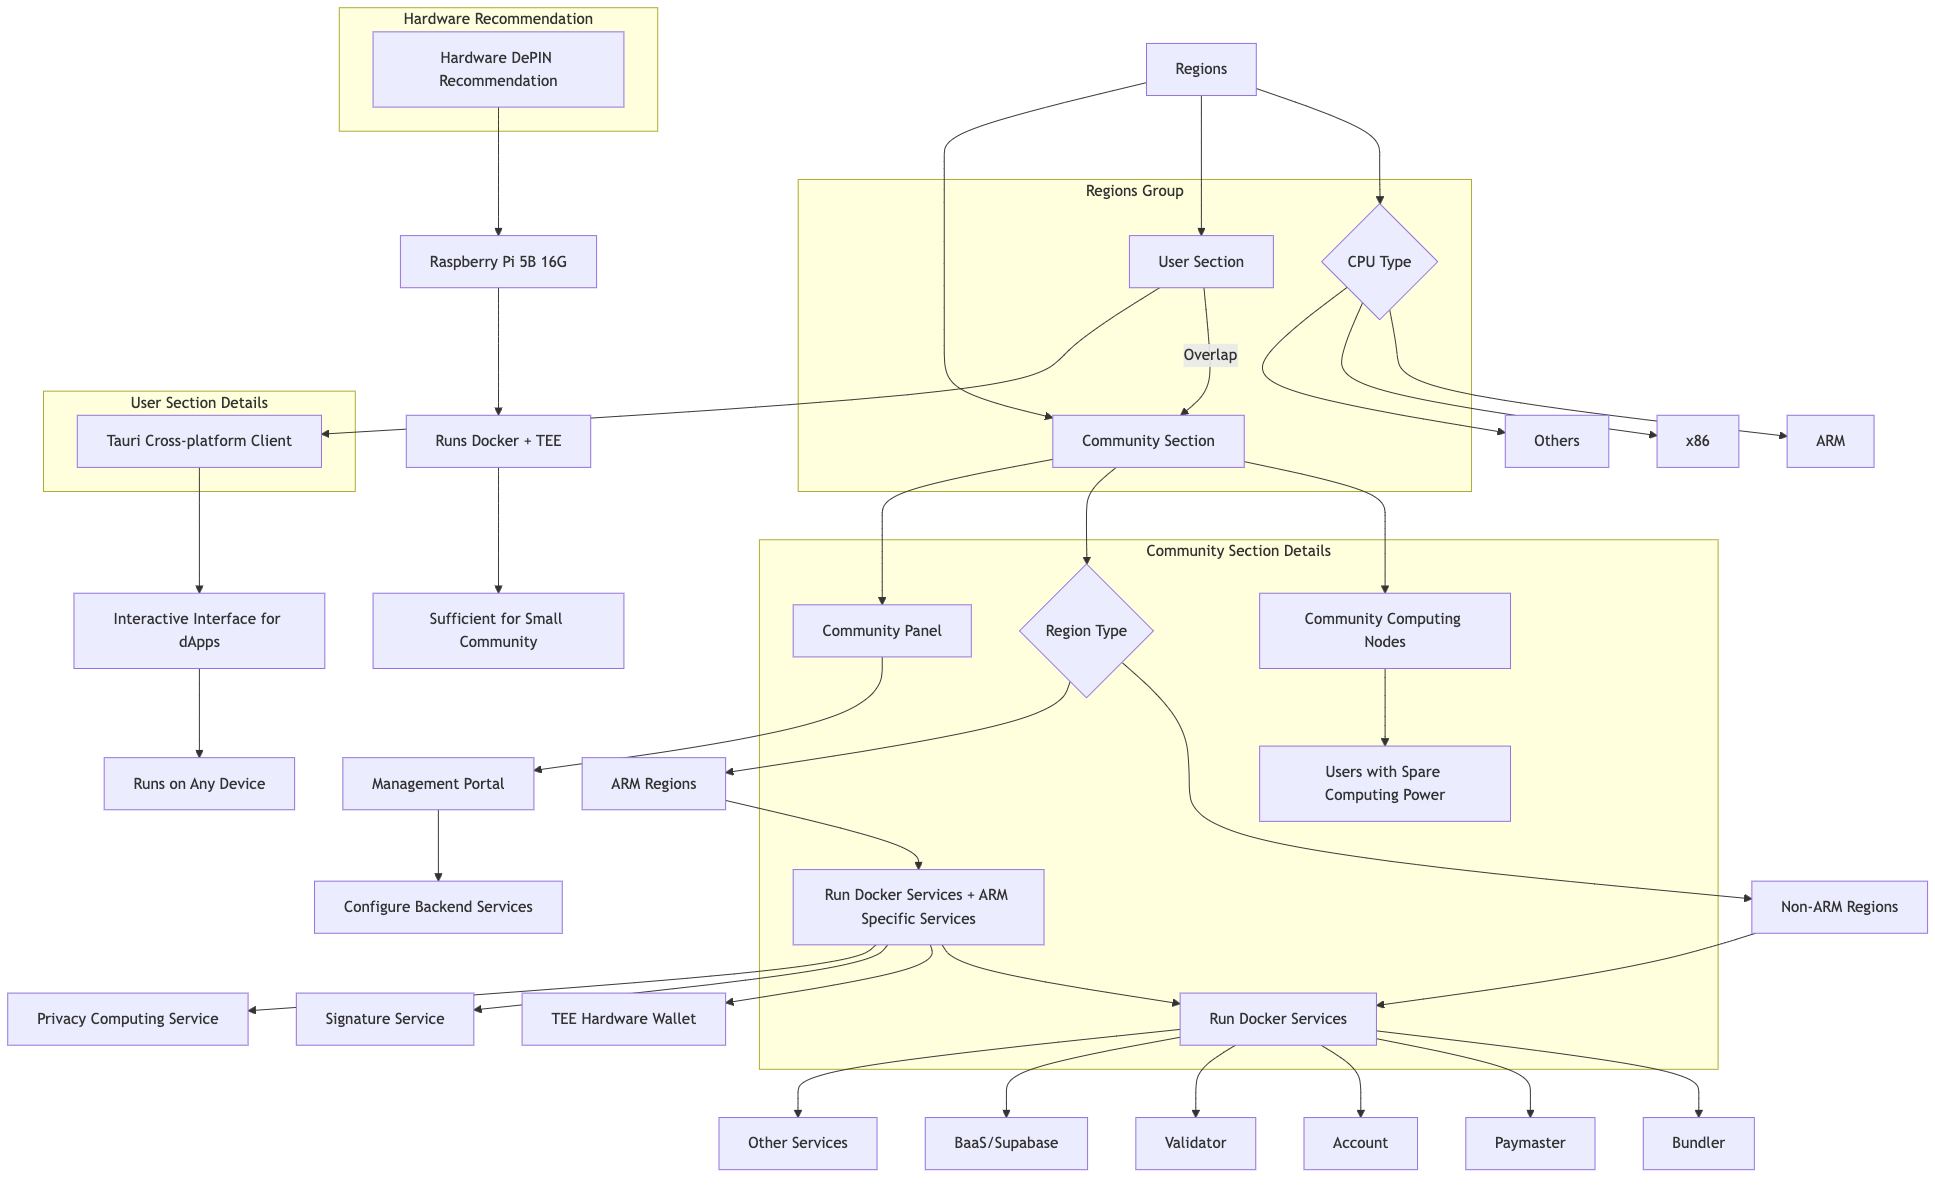
\includegraphics[width=0.8\textwidth]{backend-system-module-figure}
\caption{Backend System Module Structure}
\label{fig:backend-system-module}
\end{figure}

\section{Discussion}
\label{sec:discussion}

This section discusses how the proposed SuperPaymaster system, leveraging Account Abstraction (ERC-4337) and the Standardized Decentralized Service System (SDSS), directly addresses the usability challenges (complexity, cost, efficiency) and the risks associated with centralized gas payment solutions detailed in Section \ref{sec:analysis}.

\subsection{Countermeasures Against Usability Challenges}
\label{subsec:usability-countermeasures}

The SuperPaymaster system's design, particularly its strategic application of familiar metaphors like the 'Gas Card,' grounded in principles of social learning and Human-Computer Interaction (HCI)\cite{bandura1977,shneiderman2010,krug2009}, provides direct countermeasures to the significant usability barriers identified in Section \ref{subsec:usability-challenges}.

\subsubsection{NFT Cards (OpenCards) for Seamless Payment}

A primary usability hurdle is the cognitive load associated with understanding and managing abstract Gas concepts. The 'Gas Card' metaphor, implemented via OpenCards (NFTs/SBTs) holding OpenPNTs balances, directly tackles this by mapping the gas payment process onto the user's familiar mental model of prepaid or loyalty cards. The PoC implementation demonstrates how this reduces the perceived complexity and enhances the Perceived Ease of Use (PEOU). By automating the gas payment deduction from the card's balance via the Paymaster, the user interaction becomes seamless, approaching a "gasless" experience and significantly lowering the Gulf of Execution.

\subsubsection{Competitive Quoting for Cost Reduction}

The high and volatile cost of gas presents a major usability challenge. SuperPaymaster addresses this through its competitive quoting mechanism facilitated by SDSS. Instead of being subject to a single provider's rate or needing to manually optimize gas prices, dApps (on behalf of users) can solicit quotes from multiple decentralized Paymaster nodes. This introduces market competition, driving down sponsorship costs and providing users with more predictable and affordable transaction fees, thereby improving user satisfaction and reducing financial barriers.

\subsubsection{Community Tokens (OpenPNTs) for Low/Negative Cost}

The necessity of acquiring native tokens adds cost and complexity. The OpenPNTs framework allows communities to issue their own tokens acceptable for gas payments within the SuperPaymaster network. Combined with mechanisms for users to earn PNTs (e.g., Task-for-Points), this enables pathways to zero or even negative net gas costs for active community participants, fundamentally altering the economic aspect of the usability challenge.

\subsection{Countermeasures Against Centralization and Security Risks}
\label{subsec:centralization-countermeasures}

SuperPaymaster's decentralized architecture provides inherent advantages over the centralized gas payment solutions analyzed in Section \ref{subsec:centralized-risks}.

\subsubsection{Mitigating Monopoly and Cost Inflation}

By design, SuperPaymaster fosters a permissionless market where any entity meeting the staking requirements can operate a Paymaster node. The competitive quoting mechanism directly counteracts price manipulation and prevents long-term cost inflation associated with market monopolies.

\subsubsection{Enhancing Censorship Resistance}

Centralized relays can censor transactions based on regulatory pressure. SuperPaymaster's decentralized network of globally distributed nodes, discoverable via SDSS/ENS, significantly increases censorship resistance. Users and dApps have multiple, independent providers to choose from, making it difficult for any single entity or jurisdiction to block transactions universally.

\subsubsection{Reducing Transaction Manipulation Risks (MEV)Implications}

While MEV remains a fundamental challenge, a decentralized network of competing Paymaster nodes may reduce opportunities for systemic MEV extraction compared to a single dominant centralized relayer. Node reputation and transparent operation can further disincentivize malicious behavior.

\subsection{Implications of Findings}
\label{subsec:implications}

\subsubsection{Implications for HCI and TAM, SLT}

Assuming positive evaluation results of the 'Gas Card' metaphor validates the effectiveness of applying HCI principles, specifically metaphor design derived from social learning (SLT), to simplify complex blockchain interactions. It demonstrates how leveraging familiar mental models can significantly enhance Perceived Ease of Use (PEOU), reduce cognitive load, and potentially improve technology acceptance rates (TAM) in the Web3 domain. This study provides empirical grounding for using such user-centric design strategies to overcome usability barriers in decentralized systems.

\subsubsection{Implications for the Blockchain Ecosystem}

SuperPaymaster offers a viable blueprint for a more open, competitive, and user-friendly gas payment infrastructure. For users, they just hold a gas card and do some favor fot the community to get ERC20 PNTs to pay gas seamlessly. For dApp developers, it lowers the barrier to offering seamless user experiences without vendor lock-in. For users, it promises reduced costs and complexity. For node operators, it creates new economic opportunities. For communities, OpenPNTs/OpenCards provide novel tools for engagement and local economy building. Ultimately, such decentralized infrastructure can foster greater innovation and accelerate the mainstream adoption of blockchain applications.

\subsection{Limitations}
\label{subsec:limitations}

While the SuperPaymaster PoC demonstrates feasibility, several limitations should be acknowledged. The current implementation focuses primarily on EVM-compatible chains; cross-chain interoperability beyond basic ENS naming requires further development. The effectiveness of the Reputation Mechanism relies on robust data collection and potentially complex on-chain logic or trusted off-chain components, which needs more extensive testing under varied network conditions. The economic sustainability of the competitive market and the OpenPNTs model requires deeper analysis and real-world validation to ensure long-term viability and resistance to exploits. Furthermore, the 'Gas Card' metaphor, while beneficial for usability, might imperfectly represent underlying gas price volatility unless Paymaster nodes actively manage this risk, potentially impacting the transparency of actual costs for the user in certain edge cases. The reliance on external components like AirAccount and ENS also introduces dependencies. Finally, this research use a system design, implementation, and evaluation methodology, may not fully capture all potential real-world complexities or attack vectors present in a large-scale deployment.

\section{Related Research and Comparison}
\label{sec:related-work}

Blockchain integration in account and gas payment is widely researched; however, studies on HCI, TAM, SLT, and decentralization computing are less common. This section highlights research relevant to our proposed system. Additionally, we examine top gas payment suppliers (Pimlico, Alchemy, Stackup, ZeroDev, Coinbase, Biconomy), evaluating their solutions against various metrics to illustrate the industry's current state and and compare it with our proposed system.

General Paymaster: Singh, A. K., Hassan, I. U., Kaur, G., \& Kumar, S., introduced the basic paymaster mode: verifying paymaster, a mechanism based on ERC4337. It is a paymaster contract that verifies the signature of the off-chain paymaster relay server and then pay gas for the transaction. This contract "deployed entrypoint contract address and your offchain relay signer address as the constructor parameter values". So it can verify the signature of the paymaster server on-chain. This solution is a part of ERC4337,It provides abilities to all contract account to get gas sponsorship or gas payment by another account: paymaster. Bring a great experience to users on gas payment convinient. But it rely on a centralized paymaster server, which may be a single point of failure and risk of censorship, price manipulation and monopolization. And it is only a craft version published by ERC4337 eth-infinitism team.

% Gas Fee Analysis 表格
\begin{table}[htbp]
\centering
\begin{tabular}{|p{3cm}|p{2cm}|p{2cm}|}
\hline
\textbf{Name} & \textbf{Send ETH} & \textbf{Swap Tokens} \\
\hline
Metis Network & \$0.04 & \$0.18 \\
Loopring & \$0.04 & \$0.59 \\
zkSync Era & \$0.07 & - \\
zkSync Lite & \$0.09 & \$0.22 \\
Optimism & \$0.09 & \$0.18 \\
Arbitrum One & \$0.09 & \$0.27 \\
Boba Network & \$0.15 & \$0.17 \\
DeGate & \$0.16 & \$0.18 \\
StarkNet & \$0.19 & \$0.57 \\
Polygon zkEVM & \$0.19 & \$2.75 \\
Ethereum & \$1.10 & \$5.48 \\
\hline
\end{tabular}
\caption{Gas Fee Analysis(layer1 and layer2), data source: l2fees.info\cite{l2fees2024}}
\label{tab:gas-fee-analysis}
\end{table}

% HCI Analysis 表格美化
\begin{table}[htbp]
\centering
\footnotesize
\renewcommand{\arraystretch}{0.9}
\begin{tabularx}{\textwidth}{|c|X|X|X|X|}
\hline
\textbf{} & \textbf{HCI Literature Review Items} & \textbf{HCI Theory Items} & \textbf{Real Scenarios Questions} & \textbf{SuperPaymaster Solution} \\
\hline
1 & Trust & Evaluation Results & Role of trust & Guarantee by AirAccount: your finger-print and TEE \\
\hline
2 & Motivation & Ease of Learning, Efficiency, Memorization, Error Rate, Satisfaction & Social Learning Theory, easy to learn & Just register your ENS name and get a card, your community pay gas for your labor \\
\hline
3 & Risk & Cognitive Distribution, Tools, Environment, Social Interaction & Security and Privacy Concerns Manipulation and Censorship Risks Monopoly and Cost Issues & A competitive and decentralized gas sponsor market with affordable quota \\
\hline
4 & Perception & User Goals, System State, Execution, Intrinsic Load, Extrinsic Load, Metacognitive Load & Operational Inefficiency Asset Fragmentation Complex On-Chain Transaction Process & ENS name easy to remember and keep gas card (do nothing) \\
\hline
5 & Wallets &  & Hard to use Easy to lost money & Provide SDK for developers \\
\hline
6 & Engaging Users & Willingness to Use, Attitude, Perceived Usefulness, Perceived Ease of Use & So many barriers & Retweet and get PNTs for your gas card, negative gas cost with accumulative gas card \\
\hline
7 & Specific Application Use Cases & Activity scenarios and pain points & Memorization Difficulties Limited Gas Token Support High Cognitive Load & Enhance 7-1 step, seamlessly gas payment with OpenPNTs \\
\hline
8 & Blockchain: Support Tools & Subjects, Tools, Objects, Rules, Communities, Division of Labor & Tool support to be easy & Open-source Contract, SDK, ENS name with community support \\
\hline
\end{tabularx}
\caption{HCI Analysis\cite{frohlich2022,shneiderman2010}}
\label{tab:hci-analysis}
\end{table}

% 行业对比表横向缩放
\begin{landscape}
\begin{table}[htbp]
\centering
\footnotesize
\begin{adjustbox}{center, max width=0.98\textwidth}
\begin{tabular}{|p{2.2cm}|p{2.2cm}|p{2.2cm}|p{2.2cm}|p{2.2cm}|p{2.2cm}|p{2.2cm}|p{2.2cm}|p{2.2cm}|p{2.2cm}|p{2.2cm}|p{2.2cm}|p{2.2cm}|p{2.2cm}|p{2.2cm}|}
\hline
\textbf{Field} & \textbf{Ronan S et [1]} & \textbf{Vitalik et [2][4]} & \textbf{Singh, et.[3]} & \textbf{Qin Wang [15]} & \textbf{Lin, Z. et. [16]} & \textbf{Thibault, L [17]} & \textbf{Pimlico [5]} & \textbf{Alchemy [60]} & \textbf{Stackup [61]} & \textbf{Coinbase [63]} & \textbf{Biconomy [64]} & \textbf{Particle [54,67]} & \textbf{ZeroDev [58,66]} & \textbf{SuperPaymaster/AAStar} \\
\hline
Type & Industry & Industry & Accademic & Accademic & Accademic & Accademic & Industry & Industry & Industry & Industry & Industry & Industry & Industry & Accademic/Industry \\
\hline
Purpose & EIP2771 to support meta transaction & ERC4337 to create account abstraction\newline non-modify and surplus on current tech stack & Implementate ERC4337 solution & Discuss gas token on ERC4337 & Discuss gas cost on Layer1, Layer2 & Research on Layer2 rollup & Full ERC4337 implementation on paymaster\newline (bundler) & Combine into one solution for account\newline (wallets), gas sponsor, bundler & Service for business crypto account & Thrive the base chain ecosystem\newline with free gas sponsor & Act as a DApp infrastructure provides & Full ERC4337 implementation on paymaster\newline (bundler) and more enhancement & The most practical account abstraction & Provide a community version paymaster\newline with decentralization \\
\hline
Solution & Need every contract customize modification & alt-mempool framework with basic account abstraction flow\newline on entrypoint, bundler and paymaster & verifying paymaster on relay signature\newline and on-chain verify & easy onboarding by 3rd party payments,\newline paying with tokens & Use Layer2 to reduce the gas cost & Try to reduce gas cost, some Layer2 support\newline customize ERC20 gas token & Centralized API key with verifying and\newline ERC20 paymaster service & A top business gas sponsor service & A enterprise solution for payment\newline with gasless & Standard ERC4337 solution with strong tools\newline on Layer2 & Cross-chain paymaster service ERC4337\newline smart accounts & One token for all servicec with cross-chain;\newline Cross-chain Universal account solution. & Stay up-to-date with Ethereum updates,\newline EIP7702 and more & Cutomized community ERC20 gas token;\newline gasless account with ENS name;\newline One-key run own paymaster \\
\hline
Solution Account & EOA & Contract account demo & Contract account & Contract account & Contract account & EOA & Contract account & Contract account & Contract account & Contract account & Contract account & Contract account and EOA & Contract account & Contract account and EOA \\
\hline
Solution Relay & \ding{55} & \ding{55} & \ding{51} & \ding{51} & \ding{51} & \ding{55} & \ding{51} & \ding{51} & \ding{51} & \ding{51} & \ding{51} & \ding{51} & \ding{51} & \ding{51} \\
\hline
Solution Simple & \ding{55} & \ding{55} & \ding{55} & \ding{55} & \ding{55} & \ding{55} & \ding{55} & \ding{55} & \ding{55} & \ding{55} & \ding{51} & \ding{51} & \ding{51} \\
\hline
Solution Time/Efficiency & \ding{55} & \ding{55} & \ding{55} & \ding{55} & \ding{55} & \ding{55} & \ding{55} & \ding{55} & \ding{55} & \ding{55} & \ding{51} & \ding{51} & \ding{51} \\
\hline
Solution Customize ERC20 & \ding{55} & \ding{55} & \ding{55} & \ding{55} & \ding{55} & \ding{51} & \ding{51} & \ding{51} & \ding{55} & \ding{55} & \ding{51} & \ding{51} & \ding{51} \\
\hline
Cost Direct Cost & Low & High & High & High & Medium & Medium & Medium & Medium & Medium & Medium & Medium & Medium & Medium & Negative \\
\hline
Usability\&UX:HCI HCI:Cognitive Load & High & High & High & High & High & High & Medium & Medium & Low & Low & Medium & Low & Low & Low \\
\hline
Usability\&UX No Memorization & \ding{55} & \ding{55} & \ding{55} & \ding{55} & \ding{55} & \ding{55} & \ding{55} & \ding{51} & \ding{51} & \ding{55} & \ding{55} & \ding{55} & \ding{55} & \ding{55} \\
\hline
Usability\&UX HCI:Efficiency & \ding{55} & \ding{55} & \ding{55} & \ding{55} & \ding{55} & \ding{55} & \ding{55} & \ding{51} & \ding{51} & \ding{55} & \ding{55} & \ding{55} & \ding{55} & \ding{55} \\
\hline
Usability\&UX HCI:Fault Tolerance & \ding{55} & \ding{55} & \ding{55} & \ding{55} & \ding{55} & \ding{55} & \ding{46} & \ding{46} & \ding{55} & \ding{55} & \ding{55} & \ding{55} & \ding{55} & \ding{51} \\
\hline
Decentralization TAM:E\&E Gulf & \ding{55} & \ding{55} & \ding{55} & \ding{55} & \ding{55} & \ding{55} & \ding{55} & \ding{51} & \ding{51} & \ding{55} & \ding{55} & \ding{55} & \ding{55} & \ding{51} \\
\hline
Decentralization SLT: Society Learning & \ding{55} & \ding{55} & \ding{55} & \ding{55} & \ding{55} & \ding{55} & \ding{55} & \ding{46} & \ding{51} & \ding{55} & \ding{55} & \ding{55} & \ding{55} & \ding{51} \\
\hline
Decentralization Support & \ding{55} & \ding{55} & \ding{55} & \ding{55} & \ding{55} & \ding{55} & \ding{55} & \ding{55} & \ding{55} & \ding{55} & \ding{55} & \ding{55} & \ding{55} & \ding{51} \\
\hline
Comment & EIP2771 & AA & AA & Layer2 & Layer2 & Rollup/Layer2 & First business provider & Total solution provider & Pivot to business provider & Coinbase ecosystem & Cross-chain provider & Universal account on all-chains & Top tech solution part is close-code & Open source support self-runing,\newline Decentralized \\
\hline
\end{tabular}
\end{adjustbox}
\caption{Multi-dimensional comparison on industry general area table\cite{bundlebear2024,daian2020}}
\label{tab:industry-comparison}
\end{table}
\end{landscape}

\section{Conclusion}
\label{sec:conclusion}

Widespread blockchain adoption remains hindered by significant user challenges, primarily high gas fees, complex payment processes, and poor user experiences stemming from overly technical and centralized solutions, which deter new user onboarding. Addressing these core usability and centralization obstacles, alongside related issues in account management and security, is crucial for unlocking the full potential of decentralized applications and services.

SuperPaymaster is a novel system designed for a seamless ("gasless" perception), user-friendly, developer-accessible, decentralized, secure, and scalable gas payment system. A key contribution is the proposal of a fully competitive gas sponsorship market built upon this system. We introduce the OpenPNTs and OpenCards system, leveraging the familiar "Gas Card" metaphor. This maps the complex gas payment process onto simpler "topping up" and "paying" concepts, significantly reducing cognitive load and enhancing user experience. Furthermore, AirAccount integration provides robust decentralized second-factor authentication (D2FA), boosting security and usability during gas payment interactions. To address cryptic wallet and API addresses, CometENS enhances their readability and memorability. Underpinning the architecture is the Standardized Decentralized Service System (SDSS), facilitating relay server operation on decentralized compute nodes. This mitigates risks of price manipulation and censorship in centralized gas sponsorship services, aligning with DePIN principles through open-source solutions and permissionless registration contracts.

For future work, we plan to explore the implementation of cross-chain SuperPaymaster capabilities, including investigating interoperability with emerging Account Abstraction standards like RIP-7560\cite{rip7560} and integration with EIP-7702\cite{eip7702} to potentially support gas sponsorship for traditional Externally Owned Accounts (EOAs). Further research directions include enhancing the relay server framework by integrating AI and security policy vector models to provide more sophisticated and proactive transaction security assurances. Additionally, we intend to conduct deeper analyses of community economic models enabled by OpenPNTs/OpenCards, perform large-scale deployment and usability studies of the SDSS architecture, and continue refining the system to better serve blockchain public goods and contribute positively to the evolving human digital future.

\section{Acknowledgments}
\label{sec:acknowledgments}

This research was financed by the Plancker\^{} Community, and development was supported by the AAStar Team which was a subsidiary of Plancker\^{}.

%% The Appendices part is started with the command \appendix;
%% appendix sections are then done as normal sections
\appendix
\section{Core Components}
\label{app:core-components}

\begin{table}[ht]
\centering
\begin{tabular}{|p{2cm}|p{6cm}|p{6cm}|}
\hline
\textbf{TypeName} & \textbf{Describe} & \textbf{Repo} \\
\hline
Infra & SuperPaymaster: a universal open source paymaster contract for account abstraction. & SuperPaymaster \\
\hline
Infra & SDS: an architecture for decentralized service sponsor system. & SDSS \\
\hline
Infra & AirAccount: an open source account abstraction contract. & AirAccount \\
\hline
Infra & AirAccount-Rust-Relay: an open source relay server for AirAccount. & AirAccount-Rust-Relay \\
\hline
Infra & OpenPNTs: an open source token solution for community sustainability & OpenPNTs \\
\hline
Infra & CometENS: an open source ENS for AirAccount and SDSS. & CometENS \\
\hline
framework & HexagonWarrior: Multi OS client framework & HexagonWarrior-Tauri \\
\hline
framework & SDK and Demo: A quick Nodejs SDK and a demo to show features & AAStar\_SDK \\
\hline
\end{tabular}
\caption{Core Components}
\label{tab:core-components}
\end{table}

\section{AAStar Team}
It is a team focusing on Ethereum ecosystem, core members talked AA early with Vitalik in 2022 Moutainegro, and now working on AA and more infra over 3+ years.

\section{Plancker$^\wedge$ Community}
It is a community to help Ethereum builders, initiated by Nicolas and more guys, they help many Open-source projects in Ethereum. Incubated AAStar from 2022 to 2024 Nov.

\begin{thebibliography}{78}

% [1] Ronan Sandford, et al. (2020, July). EIP2771:Secure Protocol for Native Meta Transactions, https://eips.ethereum.org/EIPS/eip-2771
\bibitem{sandford2020}
Ronan Sandford, et al.,
\textit{EIP2771:Secure Protocol for Native Meta Transactions},
\url{https://eips.ethereum.org/EIPS/eip-2771},
2020.

% [2] Vitalik Buterin, et al. (2021, September). Account Abstraction Using Alt Mempool, https://github.com/ethereum/ercs/blob/master/ERCS/erc-4337.md
\bibitem{buterin2021}
Vitalik Buterin, et al.,
\textit{Account Abstraction Using Alt Mempool},
\url{https://github.com/ethereum/ercs/blob/master/ERCS/erc-4337.md},
2021.

% [3] Singh, A. K., Hassan, I. U., Kaur, G., \& Kumar, S. (2023, July). Account abstraction via singleton entrypoint contract and verifying paymaster. In 2023 2nd International Conference on Edge Computing and Applications (ICECAA) (pp. 1598-1605). IEEE.
\bibitem{singh2023}
Singh, A. K., Hassan, I. U., Kaur, G., \& Kumar, S.,
\textit{Account abstraction via singleton entrypoint contract and verifying paymaster},
In 2023 2nd International Conference on Edge Computing and Applications (ICECAA) (pp. 1598-1605). IEEE,
2023.

% [4] Dror Tirosh, Vitalik Buterin, et al. (2022, July). ERC 4337 team basic paymaster contract: https://github.com/eth-infinitism/account-abstraction/blob/develop/contracts/core/BasePaymaster.sol
\bibitem{tirosh2022}
Dror Tirosh, Vitalik Buterin, et al.,
\textit{ERC 4337 team basic paymaster contract},
\url{https://github.com/eth-infinitism/account-abstraction/blob/develop/contracts/core/BasePaymaster.sol},
2022.

% [5] Pimlico, a startup company invested by a16z, providing paymaster and bundler and more service. https://docs.pimlico.io/references/paymaster
\bibitem{pimlico2024}
Pimlico,
\textit{Paymaster and bundler service},
\url{https://docs.pimlico.io/references/paymaster},
2024.

% [6] Bundlebear, a account abstraction statistic website, https://www.bundlebear.com/paymasters/all, sponsored by Ethereum Foundation.
\bibitem{bundlebear2024}
Bundlebear,
\textit{Account abstraction statistics},
\url{https://www.bundlebear.com/paymasters/all},
2024.

% [7] Fröhlich, M., Waltenberger, F., Trotter, L., Alt, F., \& Schmidt, A. (2022). Blockchain and Cryptocurrency in Human Computer Interaction: A Systematic Literature Review and Research Agenda. Designing Interactive Systems Conference.
\bibitem{frohlich2022}
Fröhlich, M., Waltenberger, F., Trotter, L., Alt, F., \& Schmidt, A.,
\textit{Blockchain and Cryptocurrency in Human Computer Interaction: A Systematic Literature Review and Research Agenda},
Designing Interactive Systems Conference,
2022.

% [8] Shneiderman, B., \& Plaisant, C. (2010). Designing the user interface: Strategies for effective human-computer interaction (5th ed.). Addison-Wesley.
\bibitem{shneiderman2010}
Shneiderman, B., \& Plaisant, C.,
\textit{Designing the user interface: Strategies for effective human-computer interaction (5th ed.)},
Addison-Wesley,
2010.

% [9] Norman, D. (2013). The design of everyday things: Revised and expanded edition. Basic Books.
\bibitem{norman2013}
Norman, D.,
\textit{The design of everyday things: Revised and expanded edition},
Basic Books,
2013.

% [10] Rogers, Y. (2023). Interaction design: beyond human-computer interaction.
\bibitem{rogers2023}
Rogers, Y.,
\textit{Interaction design: beyond human-computer interaction},
2023.

% [11] Murray-Rust, D., Elsden, C., Nissen, B., Tallyn, E., Pschetz, L., \& Speed, C. (2023). Blockchain and beyond: Understanding blockchains through prototypes and public engagement. ACM Transactions on Computer-Human Interaction, 29(5), 1-73.
\bibitem{murray2023}
Murray-Rust, D., Elsden, C., Nissen, B., Tallyn, E., Pschetz, L., \& Speed, C.,
\textit{Blockchain and beyond: Understanding blockchains through prototypes and public engagement},
ACM Transactions on Computer-Human Interaction, 29(5), 1-73,
2023.

% [12] Sans, T., \& Liu, D. Z. (2024, May). Privacy-Preserving Account-Abstraction for Teams on EVM chains. In 2024 IEEE International Conference on Blockchain and Cryptocurrency (ICBC) (pp. 476-484). IEEE.
\bibitem{sans2024}
Sans, T., \& Liu, D. Z.,
\textit{Privacy-Preserving Account-Abstraction for Teams on EVM chains},
In 2024 IEEE International Conference on Blockchain and Cryptocurrency (ICBC) (pp. 476-484). IEEE,
2024.

% [13] Wood, G. (2014). Ethereum: A secure decentralised generalised transaction ledger. Ethereum project yellow paper, 151(2014), 1-32.
\bibitem{wood2014}
Wood, G.,
\textit{Ethereum: A secure decentralised generalised transaction ledger},
Ethereum project yellow paper, 151(2014), 1-32,
2014.

% [14] Buterin, V. (2013). Ethereum white paper. GitHub repository, 1(22-23), 5-7.
\bibitem{buterin2013}
Buterin, V.,
\textit{Ethereum white paper},
GitHub repository, 1(22-23), 5-7,
2013.

% [15] Wang, Q., \& Chen, S. (2023). Account Abstraction,Analysed. _arXiv.Org_, _abs/2309.00448_.
\bibitem{wang2023}
Wang, Q., \& Chen, S.,
\textit{Account Abstraction,Analysed},
arXiv.Org, abs/2309.00448,
2023.

% [16] Lin, Z., Wang, T., Zhao, C., Zhang, S., Yang, Q., \& Shi, L. (2024, February). A Measurement Investigation of ERC-4337 Smart Contracts on Ethereum Blockchain. In 2024 International Conference on Computing, Networking and Communications (ICNC) (pp. 1164-1170). IEEE.
\bibitem{lin2024}
Lin, Z., Wang, T., Zhao, C., Zhang, S., Yang, Q., \& Shi, L.,
\textit{A Measurement Investigation of ERC-4337 Smart Contracts on Ethereum Blockchain},
In 2024 International Conference on Computing, Networking and Communications (ICNC) (pp. 1164-1170). IEEE,
2024.

% [17] Thibault, L. T., Sarry, T., \& Hafid, A. S. (2022). Blockchain scaling using rollups: A comprehensive survey. IEEE Access, 10, 93039-93054.
\bibitem{thibault2022}
Thibault, L. T., Sarry, T., \& Hafid, A. S.,
\textit{Blockchain scaling using rollups: A comprehensive survey},
IEEE Access, 10, 93039-93054,
2022.

% [18] Real time estimate of L1 and L2 gas fee: https://l2fees.info/
\bibitem{l2fees2024}
L2FEES,
\textit{Real time estimate of L1 and L2 gas fee},
\url{https://l2fees.info/},
2024.

% [19] Saldivar, J., Martínez-Vicente, E., Rozas, D., Valiente, M. C., \& Hassan, S. (2023, April). Blockchain (not) for everyone: Design challenges of blockchain-based applications. In Extended Abstracts of the 2023 CHI Conference on Human Factors in Computing Systems (pp. 1-8).
\bibitem{saldivar2023}
Saldivar, J., Martínez-Vicente, E., Rozas, D., Valiente, M. C., \& Hassan, S.,
\textit{Blockchain (not) for everyone: Design challenges of blockchain-based applications},
In Extended Abstracts of the 2023 CHI Conference on Human Factors in Computing Systems (pp. 1-8),
2023.

% [20] Bandura, A., \& Walters, R. H. (1977). Social learning theory (Vol. 1, pp. 141-154). Englewood Cliffs, NJ: Prentice hall.
\bibitem{bandura1977}
Bandura, A., \& Walters, R. H.,
\textit{Social learning theory (Vol. 1, pp. 141-154)},
Englewood Cliffs, NJ: Prentice hall,
1977.

% [21] Glomann, L., Schmid, M., \& Kitajewa, N. (2019). Improving the Blockchain User Experience - An Approach to Address Blockchain Mass Adoption Issues from a Human-Centred Perspective. (pp. 608–616). Springer, Cham.
\bibitem{glomann2019}
Glomann, L., Schmid, M., \& Kitajewa, N.,
\textit{Improving the Blockchain User Experience - An Approach to Address Blockchain Mass Adoption Issues from a Human-Centred Perspective},
(pp. 608–616). Springer, Cham,
2019.

% [22] Krug, S., \& Black, R. (2009). Don't Make Me Think: A Common Sense Approach to Web Usability.
\bibitem{krug2009}
Krug, S., \& Black, R.,
\textit{Don't Make Me Think: A Common Sense Approach to Web Usability},
2009.

% [23] Blockchain industry has over 3 Trillion USD market cap: https://coinmarketcap.com/charts/
\bibitem{coinmarketcap2024}
CoinMarketCap,
\textit{Blockchain industry market cap},
\url{https://coinmarketcap.com/charts/},
2024.

% [24] Davis, F. D. (1989). Technology acceptance model: TAM. Al-Suqri, MN, Al-Aufi, AS: Information Seeking Behavior and Technology Adoption, 205(219), 5.
\bibitem{davis1989}
Davis, F. D.,
\textit{Technology acceptance model: TAM},
Al-Suqri, MN, Al-Aufi, AS: Information Seeking Behavior and Technology Adoption, 205(219), 5,
1989.

% [25] Marangunić, N., \& Granić, A. (2015). Technology acceptance model: a literature review from 1986 to 2013. Universal access in the information society, 14, 81-95.
\bibitem{maranguni2015}
Marangunić, N., \& Granić, A.,
\textit{Technology acceptance model: a literature review from 1986 to 2013},
Universal access in the information society, 14, 81-95,
2015.

% [26] Preece, J., Rogers, Y., Sharp, H., Benyon, D., Holland, S., \& Carey, T. (1994). Human-computer interaction. Addison-Wesley Longman Ltd..
\bibitem{preece1994}
Preece, J., Rogers, Y., Sharp, H., Benyon, D., Holland, S., \& Carey, T.,
\textit{Human-computer interaction.} Addison-Wesley Longman Ltd., 1994.

% [27] Helander, M. G. (Ed.). (2014). Handbook of human-computer interaction. Elsevier.
\bibitem{helander2014}
Helander, M. G. (Ed.),
\textit{Handbook of human-computer interaction.} Elsevier, 2014.

% [28] The statistics of Ethereum supply and burn for gas cost: https://usltrasound.money/
\bibitem{ultrasoundmoney}
Ultrasound.money,
\textit{The statistics of Ethereum supply and burn for gas cost:}
\url{https://usltrasound.money/}

% [29] Luger, E., \& Sellen, A. (2016, May). " Like Having a Really Bad PA" The Gulf between User Expectation and Experience of Conversational Agents. In Proceedings of the 2016 CHI conference on human factors in computing systems (pp. 5286-5297).
\bibitem{luger2016}
Luger, E., \& Sellen, A.,
\textit{"Like Having a Really Bad PA" The Gulf between User Expectation and Experience of Conversational Agents.}
In Proceedings of the 2016 CHI conference on human factors in computing systems (pp. 5286-5297), 2016.

% [30] Zarrin, J., Wen Phang, H., Babu Saheer, L., \& Zarrin, B. (2021). Blockchain for decentralization of internet: prospects, trends, and challenges. Cluster Computing, 24(4), 2841-2866.
\bibitem{zarrin2021}
Zarrin, J., Wen Phang, H., Babu Saheer, L., \& Zarrin, B.,
\textit{Blockchain for decentralization of internet: prospects, trends, and challenges.}
Cluster Computing, 24(4), 2841-2866, 2021.

% [31] Nakamoto, S. (2008). Bitcoin whitepaper. URL: https://bitcoin.org/bitcoin.pdf (: 17.07. 2019), 9, 15.
\bibitem{nakamoto2008}
Nakamoto, S.,
\textit{Bitcoin whitepaper.}
\url{https://bitcoin.org/bitcoin.pdf}, 2008.

% [32] Pacheco, M., Oliva, G., Rajbahadur, G. K., \& Hassan, A. (2023). Is my transaction done yet? an empirical study of transaction processing times in the ethereum blockchain platform. ACM Transactions on Software Engineering and Methodology, 32(3), 1-46.
\bibitem{pacheco2023}
Pacheco, M., Oliva, G., Rajbahadur, G. K., \& Hassan, A.,
\textit{Is my transaction done yet? an empirical study of transaction processing times in the ethereum blockchain platform.}
ACM Transactions on Software Engineering and Methodology, 32(3), 1-46, 2023.

% [33] Daian, P., Goldfeder, S., Kell, T., Li, Y., Zhao, X., Bentov, I., ... \& Juels, A. (2020, May). Flash boys 2.0: Frontrunning in decentralized exchanges, miner extractable value, and consensus instability. In 2020 IEEE symposium on security and privacy (SP) (pp. 910-927). IEEE.
\bibitem{daian2020}
Daian, P., Goldfeder, S., Kell, T., Li, Y., Zhao, X., Bentov, I., ... \& Juels, A.,
\textit{Flash boys 2.0: Frontrunning in decentralized exchanges, miner extractable value, and consensus instability.}
In 2020 IEEE symposium on security and privacy (SP) (pp. 910-927). IEEE, 2020.

% [34] Liu, C. W., Huang, P., \& Lucas, H. (2017). IT centralization, security outsourcing, and cybersecurity breaches: evidence from the US higher education.
\bibitem{liu2017}
Liu, C. W., Huang, P., \& Lucas, H.,
\textit{IT centralization, security outsourcing, and cybersecurity breaches: evidence from the US higher education.}
2017.

% [35] Liang, Y., Wang, X., Wu, Y. C., Fu, H., \& Zhou, M. (2023). A study on blockchain sandwich attack strategies based on mechanism design game theory. Electronics, 12(21), 4417. [36]
\bibitem{liang2023}
Liang, Y., Wang, X., Wu, Y. C., Fu, H., \& Zhou, M.,
\textit{A study on blockchain sandwich attack strategies based on mechanism design game theory.}
Electronics, 12(21), 4417, 2023.

% [36] Vermeulen, J., Luyten, K., van den Hoven, E., \& Coninx, K. (2013, April). Crossing the bridge over Norman's Gulf of Execution: revealing feedforward's true identity. In Proceedings of the SIGCHI Conference on Human Factors in Computing Systems (pp. 1931-1940).
\bibitem{vermeulen2013}
Vermeulen, J., Luyten, K., van den Hoven, E., \& Coninx, K.,
\textit{Crossing the bridge over Norman's Gulf of Execution: revealing feedforward's true identity.}
In Proceedings of the SIGCHI Conference on Human Factors in Computing Systems (pp. 1931-1940), 2013.

% [37] Solidity: A statically-typed curly-braces programming language designed for developing smart contracts that run on Ethereum. Easy to learn, high vunlunability, low performance. https://soliditylang.org/
\bibitem{solidity}
Solidity,
\textit{A statically-typed curly-braces programming language designed for developing smart contracts that run on Ethereum.}
\url{https://soliditylang.org/}

% [38] Foundry: a blazing fast, portable and modular toolkit for Ethereum application development written in Rust. High performance and easy to use. https://github.com/foundry-rs/foundry
\bibitem{foundry}
Foundry,
\textit{A blazing fast, portable and modular toolkit for Ethereum application development written in Rust.}
\url{https://github.com/foundry-rs/foundry}

% [39] Next.js: A React framework for server-rendered React applications. Support SSG and SSR and more features, The React Framework for the Web. https://nextjs.org/
\bibitem{nextjs}
Next.js,
\textit{A React framework for server-rendered React applications.}
\url{https://nextjs.org/}

% [40] React: A JavaScript library for building user interfaces. Complex but popular. https://reactjs.org/
\bibitem{react}
React,
\textit{A JavaScript library for building user interfaces.}
\url{https://reactjs.org/}

% [41] Node.js: A JavaScript runtime built on Chrome's V8 JavaScript engine. Most popular tech stack for frontend and backend development. https://nodejs.org/
\bibitem{nodejs}
Node.js,
\textit{A JavaScript runtime built on Chrome's V8 JavaScript engine.}
\url{https://nodejs.org/}

% [42] Tauri: Cross-platform desktop application framework. Create small, fast, secure, cross-platform applications, https://tauri.app/
\bibitem{tauri}
Tauri,
\textit{Cross-platform desktop application framework.}
\url{https://tauri.app/}

% [43] Go: High performance and concurrency language. Build simple, secure, scalable systems with Go https://golang.org/
\bibitem{golang}
Go,
\textit{High performance and concurrency language.}
\url{https://golang.org/}

% [44] Rust: High performance, memory safety, and concurrency. A language empowering everyone to build reliable and efficient software.https://www.rust-lang.org/
\bibitem{rust}
Rust,
\textit{High performance, memory safety, and concurrency.}
\url{https://www.rust-lang.org/}

% [45] Docker: A platform for building, shipping, and running applications. Develop faster. Run anywhere. https://www.docker.com/
\bibitem{docker}
Docker,
\textit{A platform for building, shipping, and running applications.}
\url{https://www.docker.com/}

% [46] Supabase: A open source database and authentication service. Alerternative to Google Firebase or AWS RDS and AWS Cognito. https://supabase.com/
\bibitem{supabase}
Supabase,
\textit{A open source database and authentication service.}
\url{https://supabase.com/}

% [47] An alerternative to the complex crypto account: https://github.com/AAStarCommunity/AirAccount/tree/aastar-develop
\bibitem{airaccount}
AirAccount,
\textit{An alternative to the complex crypto account.}
\url{https://github.com/AAStarCommunity/AirAccount/tree/aastar-develop}

% [48] Ballandies, M. C., Wang, H., Law, A. C. C., Yang, J. C., Gösken, C., \& Andrew, M. (2023, October). A taxonomy for blockchain-based decentralized physical infrastructure networks (depin). In 2023 IEEE 9th World Forum on Internet of Things (WF-IoT) (pp. 1-6). IEEE.
\bibitem{depin2023}
Ballandies, M. C., Wang, H., Law, A. C. C., Yang, J. C., Gösken, C., \& Andrew, M.,
\textit{A taxonomy for blockchain-based decentralized physical infrastructure networks (depin).}
In 2023 IEEE 9th World Forum on Internet of Things (WF-IoT) (pp. 1-6). IEEE, 2023.

% [49] Nielsen, L. (2013). Personas-user focused design (Vol. 15). London: Springer.
\bibitem{nielsen2013}
Nielsen, L.,
\textit{Personas-user focused design (Vol. 15).} London: Springer, 2013.

% [50] Lee, P. A., Anderson, T., Lee, P. A., \& Anderson, T. (1990). Fault tolerance (pp. 51-77). Springer Vienna.
\bibitem{lee1990}
Lee, P. A., Anderson, T., Lee, P. A., \& Anderson, T.,
\textit{Fault tolerance (pp. 51-77).} Springer Vienna, 1990.

% [51] Hollender, N., Hofmann, C., Deneke, M., \& Schmitz, B. (2010). Integrating cognitive load theory and concepts of human–computer interaction. Computers in human behavior, 26(6), 1278-1288.
\bibitem{hollender2010}
Hollender, N., Hofmann, C., Deneke, M., \& Schmitz, B.,
\textit{Integrating cognitive load theory and concepts of human–computer interaction.}
Computers in human behavior, 26(6), 1278-1288, 2010.

% [52] Julian, A., Mary, G. I., Selvi, S., Rele, M., \& Vaithianathan, M. (2024). Blockchain based solutions for privacy-preserving authentication and authorization in networks. Journal of Discrete Mathematical Sciences and Cryptography, 27(2-B), 797-808.
\bibitem{julian2024}
Julian, A., Mary, G. I., Selvi, S., Rele, M., \& Vaithianathan, M.,
\textit{Blockchain based solutions for privacy-preserving authentication and authorization in networks.}
Journal of Discrete Mathematical Sciences and Cryptography, 27(2-B), 797-808, 2024.

% [53] Bontekoe, T., Karastoyanova, D., \& Turkmen, F. (2023). Verifiable privacy-preserving computing. arXiv preprint arXiv:2309.08248.
\bibitem{bontekoe2023}
Bontekoe, T., Karastoyanova, D., \& Turkmen, F.,
\textit{Verifiable privacy-preserving computing.}
arXiv preprint arXiv:2309.08248, 2023.

% [54] Particle announcement for their token to be unified gas unit: https://blog.particle.network/celebrating-15m-end-users-debuting-our-token-centric-economy/
\bibitem{particle2024}
Particle,
\textit{Particle announcement for their token to be unified gas unit:}
\url{https://blog.particle.network/celebrating-15m-end-users-debuting-our-token-centric-economy/}

% [55] RIP 7560, a total solution for contract account and EOA account transaction(Rollup Improvement Proposal): https://github.com/ethereum/RIPs/blob/master/RIPS/rip-7560.md
\bibitem{rip7560}
RIP 7560,
\textit{A total solution for contract account and EOA account transaction(Rollup Improvement Proposal):}
\url{https://github.com/ethereum/RIPs/blob/master/RIPS/rip-7560.md}

% [56] SuperPaymaster Contract: https://github.com/AAStarCommunity/SuperPaymaster-Contract
\bibitem{superpaymaster}
SuperPaymaster Contract,
\url{https://github.com/AAStarCommunity/SuperPaymaster-Contract}

% [57] Pimilico singleton paymaster: https://github.com/pimlicolabs/singleton-paymaster
\bibitem{pimlico-singleton}
Pimilico singleton paymaster,
\url{https://github.com/pimlicolabs/singleton-paymaster}

% [58] ZeroDev bundler: https://github.com/zerodevapp/ultra-relay
\bibitem{zerodev-bundler}
ZeroDev bundler,
\url{https://github.com/zerodevapp/ultra-relay}

% [59] Pimlico Alto bundler: https://github.com/pimlicolabs/alto
\bibitem{pimlico-alto}
Pimlico Alto bundler,
\url{https://github.com/pimlicolabs/alto}

% [60] Alchemy Account Abstraction Solution: https://www.alchemy.com/account-contracts
\bibitem{alchemy-aa}
Alchemy Account Abstraction Solution,
\url{https://www.alchemy.com/account-contracts}

% [61] Stackup Account Abstraction Solution: https://www.stackup.fi/
\bibitem{stackup-aa}
Stackup Account Abstraction Solution,
\url{https://www.stackup.fi/}

% [62] Coinbase Account Abstraction Kit: https://www.coinbase.com/developer-platform/solutions/account-abstraction-kit
\bibitem{coinbase-aa}
Coinbase Account Abstraction Kit,
\url{https://www.coinbase.com/developer-platform/solutions/account-abstraction-kit}

% [63] Coinbase Bundler and Paymaster: https://portal.cdp.coinbase.com/products/bundler-and-paymaster
\bibitem{coinbase-bundler}
Coinbase Bundler and Paymaster,
\url{https://portal.cdp.coinbase.com/products/bundler-and-paymaster}

% [64] Biconomy Smart Contract Account Solution: https://docs.biconomy.io/multichain-gas-abstraction/for-sca
\bibitem{biconomy-aa}
Biconomy Smart Contract Account Solution,
\url{https://docs.biconomy.io/multichain-gas-abstraction/for-sca}

% [65] Particle Universal Account(Paymaster) Solution: https://whitepaper.particle.network/
\bibitem{particle-whitepaper}
Particle Universal Account(Paymaster) Solution,
\url{https://whitepaper.particle.network/}

% [66] ZeroDev Paymaster and Account Abstraction Solution: https://docs.zerodev.app/
\bibitem{zerodev-docs}
ZeroDev Paymaster and Account Abstraction Solution,
\url{https://docs.zerodev.app/}

% [67] Particle total solution, one account, One balance, any chain: https://whitepaper.particle.network/
\bibitem{particle-universal}
Particle total solution, one account, One balance, any chain:
\url{https://whitepaper.particle.network/}

% [68] EIP-4844 (Proto-Danksharding), Allows temparary Blob data to replace expensive calldata: https://github.com/ethereum/EIPs/blob/master/EIPS/eip-4844.md
\bibitem{eip4844}
EIP-4844 (Proto-Danksharding), Allows temparary Blob data to replace expensive calldata:
\url{https://github.com/ethereum/EIPs/blob/master/EIPS/eip-4844.md}

% [69] EIP7702, Allows Externally Owned Accounts (EOAs) with contract account ability by set the code(delegation) in their account: https://github.com/ethereum/EIPs/blob/master/EIPS/eip-7702.md
\bibitem{eip7702}
EIP7702, Allows Externally Owned Accounts (EOAs) with contract account ability by set the code(delegation) in their account:
\url{https://github.com/ethereum/EIPs/blob/master/EIPS/eip-7702.md}

% [70] EIP7691, Doubling the number of blobs per block on Ethereum, reduce L2 costs: https://eips.ethereum.org/EIPS/eip-7691
\bibitem{eip7691}
EIP7691, Doubling the number of blobs per block on Ethereum, reduce L2 costs:
\url{https://eips.ethereum.org/EIPS/eip-7691}

% [71] Evaluate All Account Abstraction Solutions: https://github.com/AAStarCommunity/EvaluationAll-AA
\bibitem{aa-eval}
Evaluate All Account Abstraction Solutions,
\url{https://github.com/AAStarCommunity/EvaluationAll-AA}

% [72] Soul Bound Token(SBT): https://vitalik.eth.limo/general/2022/01/26/soulbound.html
\bibitem{sbt}
Soul Bound Token(SBT),
\url{https://vitalik.eth.limo/general/2022/01/26/soulbound.html}

% [73] NonFungible Token(NFT): https://github.com/ethereum/EIPs/blob/master/EIPS/eip-721.md
\bibitem{nft}
NonFungible Token(NFT),
\url{https://github.com/ethereum/EIPs/blob/master/EIPS/eip-721.md}

% [74] EIP-777, a extension of ERC20, support operator role and call back methods: https://eips.ethereum.org/EIPS/eip-777
\bibitem{eip777}
EIP-777, a extension of ERC20, support operator role and call back methods:
\url{https://eips.ethereum.org/EIPS/eip-777}

% [75] EIP-2537, BLS threshold random signatures: https://eips.ethereum.org/EIPS/eip-2537
\bibitem{eip2537}
EIP-2537, BLS threshold random signatures:
\url{https://eips.ethereum.org/EIPS/eip-2537}

% [76] RIP-7212, secp256r1 support in precompiled contracts: https://github.com/ethereum/RIPs/blob/master/RIPS/rip-7212.md
\bibitem{rip7212}
RIP-7212, secp256r1 support in precompiled contracts:
\url{https://github.com/ethereum/RIPs/blob/master/RIPS/rip-7212.md}

% [77] EIP-7562, Reputation System for Account Abstraction: https://eips.ethereum.org/EIPS/eip-7562
\bibitem{eip7562}
EIP-7562, Reputation System for Account Abstraction:
\url{https://eips.ethereum.org/EIPS/eip-7562}

% [78] High perfamance edge computing node: NXP i.MX95, https://www.nxp.com/products/i.MX95
\bibitem{nxp-imx95}
High perfamance edge computing node: NXP i.MX95,
\url{https://www.nxp.com/products/i.MX95}



\end{thebibliography}
\end{document}

\endinput
%%
%% End of file SuperPaymaster.tex